\documentclass{maine-thesis}  % Default options 12pt and final copy

% Include necessary packages here
\usepackage[round]{natbib} % Load the natbib package with round brackets
\usepackage{hyperref} % Load the hyperref package 
\usepackage{setspace} % If not loaded previously for \singlespacing
\usepackage{soul}
\usepackage{booktabs}
\usepackage{amsmath} % For equations
\usepackage{tocloft} % For table of contents customization
\usepackage{graphicx}
\usepackage{longtable}
\usepackage{dcolumn}
\usepackage{ulem}
\usepackage{tabularx}



% Adjust the space between figure number and title in the list of figures
\cftsetindents{figure}{3em}{1em} % Adjust the second value to set the desired space

% Additional settings for list of tables or other lists if needed
\cftsetindents{table}{0em}{2.5em} 

%\renewcommand{\cftfigpresnum}{\hspace{2em}} % Adjust the space before the figure number
\renewcommand{\cftfigaftersnum}{\hspace{5em}} % Adjust the space after the figure number





% Creating custom commands
%\newcommand{\HIRL}{housing insecurity risk level }
\newcommand{\ct}{census tract }

\newcommand{\cts}{census tracts }

\newcommand{\hs}{housing insecurity }

\newcommand{\pct}{percent }

\newcommand{\mlr}{multinomial logistic regression }

\newcommand{\lrl}{low risk level }
\newcommand{\mrl}{medium risk level }
\newcommand{\hrl}{high risk level }

\newcommand{\lrls}{low risk levels }
\newcommand{\mrls}{medium risk levels }
\newcommand{\hrls}{high risk levels }


\setlength{\cftfignumwidth}{3em}



% Replace contents of {...} with your own information.
\title{Rurality and Robustness: Rural Communities and Housing Insecurity Risk }					% Title of thesis
\author{Steve Garcia}					% Author's name: First Middle Last
\degreesheld{A.A.S., B.A.}			% Previously earned degree(s), institution(s) and year(s).  
\degree{Data Science and Engineering}  				% Degree to be granted
\program{Spatial Information Science and Engineering}				% Degree granting department or program
\submitdate{May, 2024}				% Month and year of graduation (do not separate with a comma)

\principaladvisor[Dr. Matt Dube]{Matt Dube, Assistant Professor of Computer Information Systems} 			% Advisor's [short title and name]{name, long title}
% If you have more than one advisor then you'll should delete the first argument ("[...]") above and uncomment the following commands
%\secondadvisor{...}
%\principalshort{...} 			% Shortened advisor name for abstract.  See guidelines for example.

% Include all committee members names and titles
\firstreader{Kristen Gleason, Assistant Professor of Psychology}        
\secondreader{Sarah Walton, Assistant Professor of Sociology}


% If the thesis has MORE than one appendix, leave the following command in.  Else, comment it out.
\multipleappendicestrue 

% Begin the document.
\begin{document}
\preliminary
\titlepage

\copyrightpage[Steve Garcia]{2024}		% Optional, comment out or delete if undesired

\begin{abstract}
This thesis explores rural housing insecurity through Swope and Hernandez’s (2019) 4 C's of housing insecurity in rural areas. Little attention has been paid to rural areas in the conversation on housing insecurity and houselessness. To facilitate further discussion on this understudied issue, this exploratory study used unsupervised machine learning to group census tracts into risk levels across 7 axes of data from the American Community Survey. These were based on housing insecurity factors found in the literature. Multinomial logistic regression was used to determine variation between U.S. states based on how well state risk levels could be predicted with the national dataset. Furthermore, spatial autocorrelation analysis was employed to gauge the extent of spatial clustering within the identified risk levels and housing insecurity factors. The results indicate that many rural census tracts have a medium risk of housing insecurity, and the risk levels are hard to predict. The spatial autocorrelation results show that the housing insecurity variables were not as highly spatially clustered as expected.  
\end{abstract}

\begin{layabstract}{Housing Insecurity, homelessness, data mining}	% Replace the ... with the list of keywords
This thesis delves into the challenges of insecure housing in rural areas, drawing from Swope and Hernandez's comprehensive 4 C's framework outlined in 2019. Remarkably, rural regions have been overlooked in conversations about housing insecurity and homelessness. To shed light on this neglected issue, this investigation utilized unsupervised machine learning techniques. It categorized census tracts into risk levels across seven key data axes sourced from the American Community Survey, focusing on factors commonly associated with housing insecurity as documented in existing literature.

By employing multinomial logistic regression, the study aimed to discern variations among U.S. states, determining how accurately state risk levels aligned with the national dataset. Furthermore, spatial autocorrelation analysis was employed to gauge the extent of spatial clustering within the identified risk levels and housing insecurity factors.

The findings uncover that numerous rural census tracts exhibit a moderate risk of housing insecurity, yet predicting these risk levels proves challenging. Intriguingly, the spatial autocorrelation analysis suggests that the housing insecurity variables didn't exhibit the anticipated high levels of spatial clustering.


\end{layabstract}

\begin{dedication}
Dedicated to St. Thomas More and all who seek to build a better world.
\end{dedication}

\begin{acknowledgements}
I extend my heartfelt appreciation to the following individuals for their invaluable contributions to this research project:
    
    My advisor, Dr. Matthew Dube, who provided unwavering guidance and feedback throughout this endeavor; my committee members, Drs. Kristen Gelason and Sarah Walton, for their insightful feedback and support; my beloved wife, Katie, whose encouragement has been a constant source of motivation; Drs. Megan Smith, Jeremy Mhire, and Dolliann Hurtig, for their mentorship and guidance during my academic journey; and my grandparents, Steve and Linda Mauldin, for their wisdom and support throughout life's challenges.
    
    Your collective support has been instrumental in the success of this project, and I am sincerely grateful for your presence in my life."
\end{acknowledgements}

\pagebreak

% Commands for the required lists
\tableofcontents

\pagebreak

\listoftables	

% Include only if there are tables in the thesis
\pagebreak
\listoffigures		
\pagebreak		% Include only if there are figures in the thesis


%\listof{equations}{List of Equations}

% Sets the document spacing and pagestyle.
\mainmatter

\endinput


% Main text of the thesis.  Use of the `\input' command will make later editing much easier.
\chapter{Introduction} 

%\subsection{\textit{Background}}
Homelessness research has undergone a significant transformation in recent years. Historically, the focus was on categorizing and describing different segments of the homeless population \citep{lee_homelessness_2021}. A contemporary approach views homelessness as a spectrum rather than a binary condition (e.g., Desmond et al., 2015; Swope and Hernandez, 2019). This paradigm shift creates opportunities to address homelessness and housing insecurity. Four critical areas remain unaddressed in the literature. First, housing research has concentrated on urban settings resulting in an urban-centric view of social issues like poverty and homelessness. Second, measuring housing insecurity is challenging because of its dependence on circumstances and obstacles for both individuals and communities \citep{leifheit_building_2022}. Third, housing and homelessness in urban and rural areas necessitate a multi-disciplinary approach to properly capture the aspects that contribute to them, an approach rarely used in the extant literature.  Finally, the scarcity of identified community-level risk factors in rural areas coupled with a dearth of rural-specific data and research, limits our understanding of housing insecurity and rural homelessness \citep{gleason_using_2021}. Studies on homelessness often focus on descriptive surveys of those accessing public services and providers of public services \citep{robertson_rural_2007}. Addressing these gaps by integrating rural areas into the discourse on homelessness and housing insecurity is essential for creating a just and equitable society with effective policies for preventing and addressing homelessness\citep{oregan_how_2021}.

\section{\textit{Rural Areas}}

 Rural areas encompass a broad spectrum of places, including farms, ranches, villages, small towns, and many other qualities \citep{cromartie_defining_2008}. \citet{castle_conceptual_1998} identified a sparse population, interdependence with urban and global systems, and enormous diversity as three general characteristics of rural places.  At their core, rural areas are a function of "space, distance, and relative population density" \citep[?]{castle_place_2011}.\citet{shoup_principles_2010} group urban areas into three categories: rural areas dependent on nearby urban centers, "destination counties" with natural or artificial amenities that attract non-permanent residents, and production communities that revolve primarily around a single industry. This variation makes defining and understanding rurality a difficult challenge. Rural areas dominate the land mass of the United States, but with 85 percent of the population living in urban areas, they are often overlooked in the public discussion \citep{pendall_future_2016}. Despite this variation in rural areas,  "rural" is often defined as "not urban" 
 \sout{(National Coalition for the Homeless, 2009)}. In the study of housing, rural areas are almost entirely excluded from the conversation \citep{gkartzios_housing_2017}. Contributing significantly to this problem is a wide variety of definitions used by governmental organizations, policymakers, and scholars (\citealp{yousey_defining_2018}; \citealp{cromartie_defining_2008}). Recently, The main policy objective for rural communities has been the promotion of economic development and preservation of the characteristics ascribed to rural areas \citep{lichter_changing_2007}. 

Rural people make up about 20 percent of the nation's population. They make up 13 percent of the metropolitan population, 48 percent of the micropolitan population, and 75 percent of the noncore-base area population \citep{isserman_national_2005}. As Figure~\ref{fig:pop_map} demonstrates, the size of rural areas compared to the population density is vast. Deconstructing the urban-centric lens of housing research necessitates a novel approach that can accommodate the differences in rural areas. The size and variation necessitate addressing rural issues differently because there can be no one-size-fits-all policy approach to improving conditions for rural people. 

\begin{figure}[htbp]
    \centering
     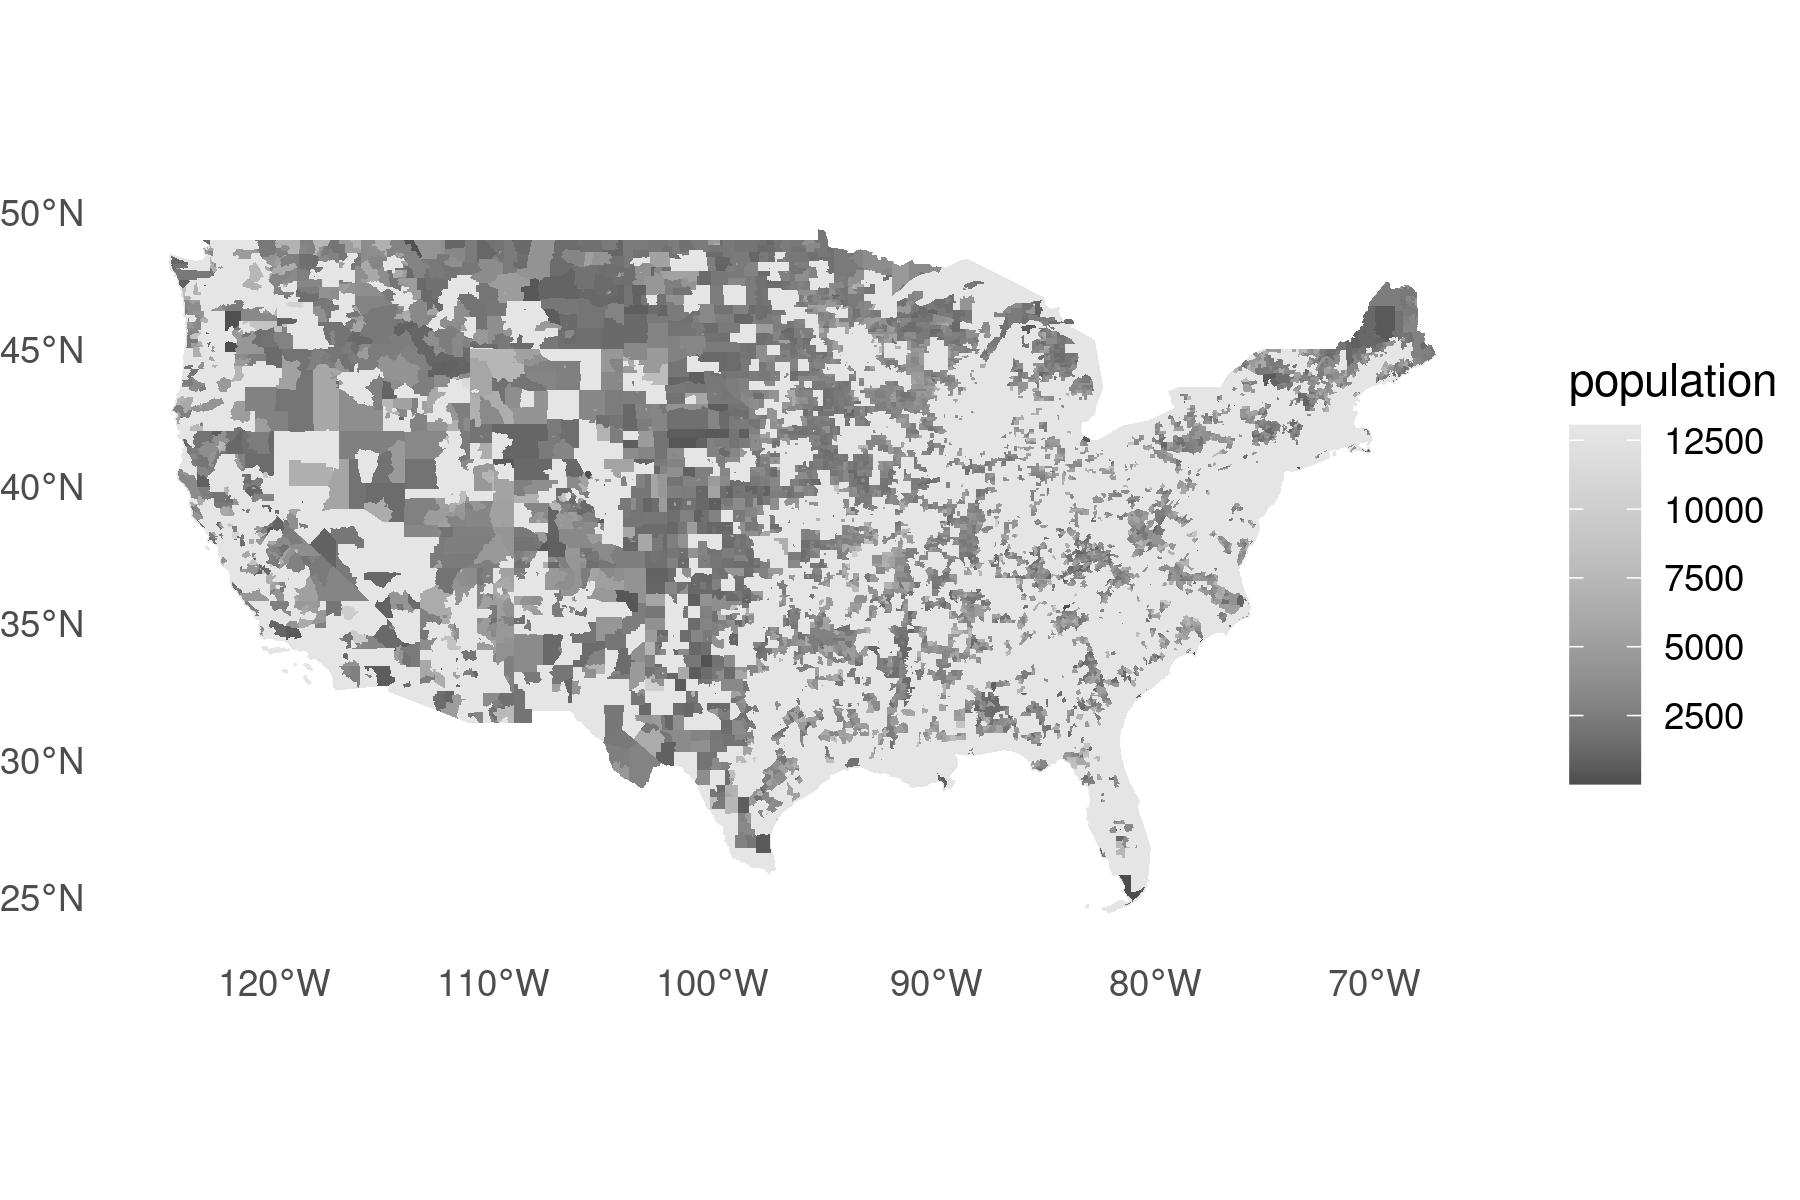
\includegraphics[width=1\textwidth, height=10cm]{plots/pop_map.png}
     \caption{Rural Population Density}
     \label{fig:pop_map}
 \end{figure}


\section{\textit{Literal Homelessness}}
For decades, scholars have debated if research should focus on the reasons why people become homeless or the structural forces that create homelessness \citep{shlay_social_2003}. Prior to significant shifts in the 21st century, research on homelessness focused on identifying and describing categories of homeless people \citep{lee_homelessness_2021}. Much research has focused on the binary of individuals and families being housed or unhoused and trying to assign them into umbrella categories. This neglects the wide range of individual and societal factors that occur in the phases between when a household is housed and becomes unhoused. Estimating the number of unhoused people is notoriously difficult even in urban areas. For measuring homelessness, the most popular mechanism for measuring homelessness in the United States is the Department of Housing and Urban Development (HUD) point-in-time (PIT) count and housing inventory count. These counts are used for the distribution of federal funds for combating homelessness. As \citet{agans_enumerating_2014}  note, the unhoused frequently relocate and the housed may quickly become unhoused, making it difficult to accurately estimate the number of unhoused people at any given time. When it comes to addressing literal homelessness, public health experts differentiate between preventative services and reactive or emergency services \citep{oregan_how_2021}. Preventive services prevent households from becoming homeless, while reactive or emergency services step in after a household becomes homeless. A common reactive program is a treatment program where an unhoused person is required to participate in short-term residential programs before being placed in more permanent housing \citep{evans_reducing_2019}. As homelessness is often seen as an urban problem, most intervention occurs in urban areas \citep{gleason_using_2021}. Significant federal action on homelessness began with the passage of the McKinney-Vento Homeless Assistance Act of 1987. it provided funds to support a variety of programs  \citep{evans_reducing_2019}. The HEARTH Act of 2009 expanded the definitions of homelessness for supported federal programs to expand those eligible beyond the literal homeless. These included those living in a place that is not meant for habitation, people who are expected to lose their residence within 14 days, families with children that are unstably housed, and people fleeing domestic violence  \citep{evans_reducing_2019}. % need to break up the use of the same source here


\section{\textit{Housing as Health}}
A house is far more than four walls, a roof, and some doors. The characteristics and location of a house have a significant impact on one’s life. In the United States, housing is often a family’s greatest expenditure, greatest source of wealth, and a place of safety and gathering \citep{braveman_housing_2011}. The federal government has long acknowledged this through legislation like the Housing Act of 1949, and social programs and development goals developed by HUD. Housing is often seen as one of the most fundamental determinants of health and a lack of adequate housing can produce adverse health outcomes and acts as a foundation for “social, psychological, and cultural well-being” (\citealp[p.17]{dalessandro_housing_2020}; \citealp{leifheit_building_2022}).  A health disparity or health inequity is a difference in health or health outcomes as they relate to social, political, and economic factors \citep{lutfiyya_rurality_2012}. One major factor that has been linked to health disparities is income, and this relationship exists across a wide range of socioeconomic factors \citep{canto_rural_2014}.  Part of acknowledging housing as health is moving beyond the housed/ unhoused binary in order to better understand and intervene in households that are at risk of becoming unhoused. This is often referred to as housing insecurity, a broader term that encompasses a continuum that affects a larger part of the population than simply housed/ unhoused \citep{deluca_housing_2022}.

\section{\textit{Theoretical Framework}}

Rather than focusing on literal homelessness, this thesis approaches housing from a housing insecurity perspective. Housing insecurity has a variety of definitions across government organizations, but it can be characterized as housing stability, housing affordability, housing quality/ safety, and neighborhood quality/ safety \citep{cox_road_2019}. To further refine these broad characteristics, this thesis follows the 4 C's approach to housing insecurity. With little infrastructure for homelessness services in rural areas, the 4 C’s approach to housing insecurity proposed by \citet{swope_housing_2020} can highlight areas of critical concern for devoting resources to reactive services and identify areas where preventative services can improve or expand. The pillars of the 4 C's include conditions: the quality of housing, cost: the affordability of housing, consistency: residential stability, and context: neighborhood opportunity.

The 4 C’s of housing are an interconnected web of factors that impact health and encapsulate the “unequal distribution of housing disparities along other axes of inequality, and the historical forces shaping unequal housing opportunities” \citep[1]{hernandez_housing_2019}.  Swope and Hernandez are not the only scholars to design a model encompassing these 4 factors. \citet{metzger_fair_2017} proposed a similar framework that encompasses stability, affordability, internal housing conditions, and area characteristics. That multiple scholars have conceptualized a similar approach indicates that it may adequately encapsulate housing insecurity

\section{\textit{Motivation}}
Three primary reasons motivate this thesis:

The first motivation stems from the lack of attention scholars have paid to rural areas as it pertains to housing insecurity. While the literature on rural housing insecurity is growing, there has yet to be a holistic nationwide survey of rural housing insecurity. Rural areas deserve more attention, and this thesis hopes to serve as a starting point for future research on rural housing insecurity at all levels with the ultimate goal of breaking the urban-focused lens of housing insecurity.

The second motivation is to test the efficacy of the 4 C's model of housing insecurity in the rural United States. With the urban lens to housing insecurity, an adequate theoretical model must be capable of adapting to areas often left out of the conversation. One study \citep{gleason_using_2021} has applied the 4 C's model to housing insecurity in the state of Maine. Most applications of the 4 C's have been to study the relationships between various conditions and housing insecurity, but no studies have applied it broadly to rural housing insecurity.

The final motivation is to provide policy-makers and researchers with a framework to identify rural areas of housing insecurity in their constituency and create harm reduction approaches and services that can meet the unique needs of their areas. The patchwork of local, state, and federal systems that encompass the aid programs of the United States means that many people involved in the policy-making process with no adequate mechanism for addressing housing insecurity in their particular jurisdictions.

\section{\textit{Approach}}
In order to improve our understanding of rural housing insecurity, this thesis investigates the risk levels of rural census tracts in the United States under the 4 C's model of housing insecurity. Risk factors across eight different axes are used to assign risk levels to rural census tracts with k-medoids clustering used to assign risk levels. Each state is clustered with census tracts from other states within a 15-mile boundary to encapsulate how communities exist across state lines. The cluster medians are analyzed to understand the trends in housing insecurity factors across states and the clusters are relabeled based on risk factors identified in the literature so that each cluster falls into a low, medium, or high-risk level. These risk levels are used to highlight census tracts at a high and medium risk of housing insecurity. Association rules learning is used to identify common patterns between sector risk levels and identify pockets of rural census tracts that are at high risk of housing insecurity. To better understand how factors of housing insecurity relate to space, Moran's I spatial autocorrelation is used to determine how spatially clustered each housing insecurity factor and sector is. Local Moran's I is used to determine how spatially clustered each risk level is to better understand the clustering of housing insecurity risk in rural areas. Finally, a multinomial logistic regression is used to determine how well each state's sector risk levels can be predicted, and a national model is generated for each sector's risk levels to analyze well the risk levels created by this implementation of the 4 C's model can be predicted nationally and state by state. 

Beginning to understand rural homelessness requires that several questions be answered: How can risk factors be used to identify risk levels of housing insecurity while accounting for the variation in rural areas and what do the risk levels say about rural areas? When measuring housing insecurity across different dimensions, how often do the same features arise? Are there spatial relations between the different dimensions of housing insecurity? To what extent can this model of housing insecurity be used to predict risk levels across housing insecurity factors?

\section{\textit{Major Results}}

The work presented in this thesis presents a novel application of the 4 C's of housing insecurity framework and applies it to rural areas. This framework allows for the identification of 776 rural census tracts with a high or medium risk of housing insecurity. It also presents evidence that clustering of housing insecurity factors may not be as common in rural areas as they are in urban areas. Due to its exploratory nature, the results are primarily intended to be used as a starting point for future research into rural housing insecurity. 

\section{\textit{Intended Audience}}
This thesis is intended for an audience with a significant interest in rural housing insecurity. Such an audience can include but is not limited to policymakers, economists, political scientists, community psychologists, rural sociologists, and many others concerned with housing insecurity. 

\section{\textit{Structure of Thesis}}
The thesis is structured into six chapters. Chapter 2 offers a comprehensive theoretical foundation, focusing on the application of the 4 C's of the housing insecurity model. This chapter reviews pertinent literature on various facets of the model. Chapter 3 explains the methodology employed for data processing. It provides an in-depth explanation of the chosen methodology and its execution. The ensuing Chapter 4 presents the study's findings, offering a detailed analysis of the acquired results. Chapter 5 deliberates on the implications of the results, discussing their significance and impact within the scope of the study. This chapter provides a thorough examination of the noteworthy findings. Chapter 6 serves as a synthesis, summarizing the entirety of the work and offering insightful commentary on the major findings. Additionally, it highlights potential avenues for future research and study.

\endinput				
\chapter{Background}	%Chapter title


% TODO: I need to figure out which desmond_forced_2015 citations belong to the two different articles  
There are three primary areas where the extant literature must be analyzed. First,  it is important to understand the distinction between homelessness and housing insecurity. Next, it is necessary to take a multi-disciplinary look at each pillar of the 4 C's of housing insecurity. Finally is the unique challenges that face rural areas in order to better inform the theoretical framework. Together, these 3 aspects form the theoretical basis for exploring rural housing insecurity.

\section{\textit{Housing Insecurity}}

Housing insecurity is a term that stems from the shift in homelessness research from focusing on only the housed and the unhoused. %The Oxford Dictionary defines housing insecurity as "the state of not having stable or adequate living arrangements, especially due to risk of eviction or because one lives in unsafe or uncomfortable conditions" \hl{(Source)}.
 \citep{deluca_housing_2022} argue that the term housing insecurity is a more dynamic concept than the traditional housed and unhoused binary. "Housing insecurity operates through multiple mechanisms-including material hardship, stress, environmental and infectious disease exposures, social network disruption and barriers to healthcare- to produce adverse health outcomes over the life course" \citep{leifheit_building_2022}. Housing insecurity as an area of study can be seen as a natural evolution stemming from researchers moving beyond the housed and unhoused binary. Homelessness is generally attributed to poverty and a lack of access to affordable housing \citep{noauthor_rural_2009}.  As researchers shifted away from the housed and unhoused binary, identifying characteristics that distinguish the housed from the unhoused began to identify factors that occur on the path to homelessness \citep{phelan_social_2010}.  The identification of these factors likely contributed to the rise of housing insecurity as a term and as a field of study.  \citet{deluca_housing_2022} argue that housing insecurity may be a more useful term than the housed and unhoused binary because it acknowledges housing hardship and housing risk as a continuum that affects a wider section of the population than literal homelessness.  One issue with the study of housing insecurity is that, similar to the concept of rurality, a wide variety of definitions are used. Cox et al. (2019) analyzed 106 studies and found that current approaches to housing insecurity have three major issues: a lack of a uniform definition, it is often applied as an underdeveloped concept, and it is often measured inconsistently. An explanation for this variation is that housing insecurity operates through a variety of mechanisms \citep{leifheit_building_2022}.  Rather than giving a strict definition, it may be more beneficial to look at the dimensions of housing insecurity. \citet{cox_road_2019} identifies seven dimensions of housing insecurity: housing stability, housing affordability, housing quality, housing safety, neighborhood safety, neighborhood quality, and literal homelessness. To adequately address housing insecurity it is necessary to have a theoretical framework that can encompass these different dimensions to avoid these pitfalls. 

\section{The 4 C's of Housing Insecurity}

To understand housing insecurity in the context of the 4 C's framework, the following subsections detail each pillar of housing insecurity under the model proposed by \citep{hernandez_housing_2019}. As each pillar forms a web rather than separate pieces, there is a significant amount of overlap between pillars. The pillars meet the dimensions identified by \citet{cox_road_2019}: housing stability (consistency), housing affordability (cost), housing quality/ housing safety (conditions), and neighborhood safety/ neighborhood quality (context). 
 
\subsection{\textit{Cost}}
Housing costs are generally conceived as the amount of a households budget that goes to housing. This includes rent or mortgage payments, utilities, and other expenses. A cost-to-income ratio is the most common way of measuring housing affordability. It is difficult to determine one number that determines when a household is spending too much on housing. The threshold for housing affordability has varied between 25 and 50 percent with the current standard set at 30 percent \citep{kropczynski_insights_2012}.  Housing is considered affordable if the household spends less than 30 percent of its income on housing and 50 percent or more is considered a high-cost burden (\citealp{braveman_housing_2011}; \citealp{swope_housing_2020}; \citealp{weicher_housing_2006}). Inherent to a cost-to-income ratio is the understanding that there are other expenses necessary for survival \citep{herbert_measuring_2018}. 
%Housing costs are determined by the rate of household formation and household attrition \citep{pendall_future_2016}.  
Housing affordability affects individuals, families, and communities while access is largely determined by their demographic characteristics  (\citealp{braveman_housing_2011};\citealp{yadavalli_comprehensive_2020}). Housing affordability is directly related to residential stability and has the potential to harm both those being forced to move, the community they are leaving, and the community they are entering \citep{desmond_forced_2015}. Access to affordable housing affects the physical and material comfort of communities and individuals. If a household cannot afford to live in their current place, they may be forced to relocate seeking more affordable housing voluntarily or through eviction and foreclosure.  If too much of a household’s money goes to housing, they may be forced to go without other necessities \citep{herbert_measuring_2018}. Those with high housing costs may also experience food insecurity as food is often considered a flexible expense while housing is a fixed expense (\citealp{fletcher_assessing_2009}; \citealp{kropczynski_insights_2012}). This is only one area where low-income households may have to compromise in order to maintain their fixed housing costs. Housing is often the biggest expense for low-income families, forcing them to make trade-offs between housing and other necessities \citep{desmond_housing_2015}. The shortage of affordable housing drives lower-income families to substandard housing in worse neighborhoods \citep{braveman_housing_2011}. This creates the potential for a spiral where housing instability cannot be escaped due to the added costs of moving. \citet{kang_severe_2021} characterizes housing instability as a by-product of the affordable housing shortage wherein households can be destabilized by minor financial shocks. These factors can create a situation where housing costs lead to residential instability, which is linked to a variety of adverse conditions, especially in children and adolescents \citep{desmond_forced_2015}. Housing affordability is both influenced by and exerts influence on many other aspects of life, and its relationship to housing insecurity cannot be understated. % rephrase last sentence 

\subsection{\textit{Conditions}}

Internal housing conditions have been identified as a significant factor on health (\citealp{braveman_housing_2011}; \citealp{metzger_fair_2017}; \citealp{swope_housing_2020}). In one study, decent housing was found to be a more important determinant of health than education or income \citep{angel_housing_2014}. Previous environmental health research has identified five broad categories in which housing conditions contribute to adverse health effects: physical conditions, chemical conditions, biological conditions, building and equipment conditions, and social conditions \citep{jacobs_environmental_2011}. Links to an increase in disease have been tied to poverty, poor housing, and degraded environments reflecting the interconnectedness of housing insecurity issues \citep{rauh_housing_2008}.  \citet{angel_housing_2014} found that the probability of facing a chronic disease increases when housing problems accumulate and that poor housing conditions quickly degrade subjective health. These problems are amplified in the modern world where individuals spend an estimated 90 percent of their time indoors \citep{palacios_impact_2021}. The relationship between housing conditions and poverty and the range of categories that contribute to housing conditions emphasize the importance of viewing housing as a matter of health. Housing conditions also play a role in residential mobility as \citet{desmond_housing_2015} place decent housing and affordable housing as fundamentally connected and the previously mentioned rise in housing cost has not brought an increase in housing quality. The impacts of housing conditions on health means that adequate housing is a public health issue \citep{matte_housing_2000}. Despite housing conditions playing such a significant role in modern life, there is not a significant sense of communal benefit and responsibility when it comes to housing \citep{jacobs_environmental_2011}.  Without a sense of communal benefit towards housing, this leaves marginalized populations that are more likely to be exposed to harmful housing conditions without community support \citep{swope_housing_2020}. Growing a sense of communal benefit towards housing would be beneficial for all aspects of housing insecurity. 

\subsection{\textit{Consistency}} 

Residential mobility is a complicated subject because, as a broad concept, it is conceived as a good thing. That one can pack up and go somewhere with more opportunity is considered a part of the American “mystique” \citep{molloy_internal_2011}. An average of 15 percent of Americans move every year and 25 percent move over two years \citep{bachmann_ins_2014}. Classic urban economic theories hold that households make trade-offs between proximity to jobs and housing prices \citep{hu_housing_2019}. This puts low-income households at a disadvantage as their access to jobs may be lower than their wealthier counterparts. Consistency or residential stability plays an important role in the physical and social well-being of individuals, families, and communities. It has been linked to a variety of adverse conditions and affects the neighborhoods being entered and left. It has been identified as a more important predictor of community health than standard factors like poverty and racial composition (\citealp{desmond_forced_2015};\citealp{desmond_housing_2016}, \citealp{rauh_housing_2008}). An important distinction must be made between voluntary and involuntary moves \citep{siskar_who_2019}. While most moves are voluntary, millions of low-income households struggle to maintain housing stability (\citealp{phinney_exploring_2013}; \citealp{kang_why_2019}). Outside of voluntary moves foreclosure, eviction, and condemnation are all drivers of forced relocation (\citealp{phinney_exploring_2013}; \citealp{siskar_who_2019}). It is linked to an increase in residential instability and households forced to move often end up in places with greater disadvantage and are more likely to face additional moves \citep{desmond_forced_sholl_2015}. One issue with the study of residential mobility is the limited scope of predictors that have been linked to it \citep{kang_why_2019}. One group at a higher risk of housing instability are those who rent their housing. Renters are particularly vulnerable to relocating to worse neighborhoods than the ones they are exiting \citep{desmond_forced_2015}. Residential instability is closely related to housing affordability, reinforcing the idea that housing insecurity is an interconnected web.

\subsection{\textit{Context}}

Context revolves around neighborhood and community characteristics including demographics, green spaces, education, and healthcare among other things. While it is impossible to capture context in its entirety, this thesis focuses on demographics, employment, housing type, and household factors as these have all been studied as matters related to housing insecurity that do not fall directly into the other pillars. The following is an interdisciplinary review of how these selected factors affect housing insecurity.  

\subsubsection{\textit{Employment}}

In the United States, the labor market is the result of cumulative individual behaviors including geographical migration and educational investments \citep{wiener_labor_2020}. The demand for labor is driven by firms, which must consider a wide variety of factors in deciding location \citep{partridge_persistent_2007}. In recent decades, the United States labor market has entered a risk regime job market where workers hold a greater share of the risk in an employment system without the perceived promise of security and stability, which has become embedded in American social and political institutions \citep{lowe_perceived_2018}. It is agreed that the Fordist regime that brought unprecedented prosperity in the early 20\textsuperscript{th} century came to an end in the 1970s \citep{stockhammer_stylized_2008}. Since this shift, the productivity of the average worker has increased by 64.6 percent while hourly pay has only increased an average of 17.3 percent between 1979 and 2021 \citep{productivity-pay-gap_2022}. Over this same period, HUD data show that the median price of a new single-family home increased from \$60,600 (\$232,091 adjusted for inflation) in 1979 to \$369,800 in 2021 \citep{us_census_bureau_median_1963}. These shifts in the housing market are one of the underlying factors in the rise of the affordable housing shortage. As wages have failed to keep up with the price of housing, the current economic system under this risk regime places those with low incomes in a precarious situation for housing affordability and residential stability. The Great Recession has had a lasting impact on the housing market within the United States. As the economic recovery did not benefit all households equally, wealth inequality has grown along both racial and ethnic lines \citep{kochhar_wealth_2014}. Thus, employment insecurity and income inequality are two pressing issues the United States is facing that have serious impacts on communities. “housing insecurity has risen in relative lockstep with employment insecurity” \citep[48]{desmond_housing_2016-1}. Economic conditions play a significant role in housing insecurity because adequate income, usually through employment, is critical for all aspects of housing insecurity. 


One significant cause of employment insecurity is a lack of economic diversity, generally caused by a lack of economic development. \citet{sherrieb_measuring_2010} identify three key elements connected to economic development: the level of economic resources, the level of equality in resource distribution, and the level of diversity in economic resources. Economic development alongside demographic change in rural areas has been linked to the quality and condition of local housing infrastructure \citep{barcus_heterogeneity_2011}. How policies shape economic development has a direct effect on the overall housing insecurity risk of rural communities. Amid the recent major economic shifts, globalization and shifting employment sectors play a critical role in the development path of communities which has an inherent effect on the people who live there \citep{harrison_spatial_2019}. Demonstrating the interconnectedness of communities, regional economic development in one area can encourage economic stability of its neighboring regions as well so it is important to view communities as interrelated rather than separate entities \citep{chen_economic_2018}. \citet{deller_spatial_2016} highlight the importance of economic diversity, a vital aspect of economic development, finding that more diverse economies enhance economic stability. As an insulator against economic instability, employment diversity is a key factor that policy-makers and scholars should consider as part of a holistic approach to housing insecurity. 

\subsubsection{\textit{Housing, race, and poverty}}

Housing is affected by a variety of social, political, and economic factors. “The ability of residents to access affordable housing, whether renting or buying, is in large part determined by their demographic characteristics, such as income, race, age, and educational attainment” \citep[115]{yadavalli_comprehensive_2020}. While unpredictable events may narrow the disparities, “As a rule, a household’s vulnerability to displacement should be shaped in a predictable fashion by those characteristics that define its members’ position in the [social] stratification system” \citep[5]{lee_forced_2020}. This vulnerability is driven by a combination of individual and socio-demographic factors. One major factor that has made minorities vulnerable to housing insecurity is discrimination in housing. Although the federal government took a direct interest in promoting home ownership in 1933, racial discrimination in the housing market was not outlawed until 1968 and enforcement of the law remained difficult until the Fair Housing Act of 1988 \citep{sharp_emerging_2014}. For example, the practice of redlining made it difficult for Black Americans to receive mortgages under federal aid programs and created racial segregation that can still be seen today. At the county level, the probability of living in affordable housing decreases as the white population decreases (Brooks, 2022). In addition to racial segregation, income segregation must be considered for a holistic discussion of housing insecurity. A high concentration of poverty may exacerbate housing condition issues due to a lack of revenue to maintain the necessary services at the household and local government levels. Minorities are also at a disadvantage in income segregation with poor whites being less segregated from their non-poor counterparts \citep{lichter_ruralurban_2021}. As a home is often a household's greatest source of wealth, the disadvantages minorities have in terms of housing are compounded as social and economic inequality are reproduced as these disparities continue \citep{krivo_housing_2004}.  

\subsubsection{\textit{Housing Type}} 

While owning a home is considered a part of the “American Dream,” many households rent their housing by choice or by necessity. While the many benefits of home ownership portray it as a means to a better life, renting is not inherently bad and may provide better opportunities for households that can afford it, but there are many potentially destabilizing consequences of high-cost renting \citep{drew_believing_2014}. Nationally, the median rent in a poor neighborhood is higher compared to a middle-class or affluent neighborhood after regular expenses are deducted despite property values typically being much higher in middle-class or affluent neighborhoods \citep{desmond_poor_2019}. This creates a compounding factor for the previously mentioned disparities in home ownership. Increases in household wealth and secured debt were found to decrease the likelihood of homeowners becoming renters and vice versa \citep{anderson_effect_2021}. Renters with high-cost housing are unable to increase household wealth through their means of housing.  In addition to whether one rents or owns a home, the type of home can play a significant role in housing insecurity. Of particular concern is unconventional housing which includes dwellings not considered long-term habitation including RVs/ campers, vans, and boats. These unconventional forms of housing may keep people off the streets, but they are not always a stable mode of housing. For RV and camper living, people who are undocumented or are unable to keep up with legal or maintenance costs for vehicles end up losing their housing \citep{wakin_not_2005}. Those who rent with a high housing cost and those who live in unconventional housing should be considered to have a high risk of housing insecurity. In rural areas, mobile homes are often seen as an affordable option but they come with certain risks not as common in traditional housing. Structural problems like poor construction and risks of air pollution and fire create a unique problem \citep{mactavish_policy_2006}. Mobile homes also carry a unique set of circumstances that may put households at a greater risk of housing insecurity and are found frequently in rural areas. Mobile homes and the land they are situated on can be either owned or rented. It is common in mobile home parks for households to own their home but not the land it is on. Key issues with mobile homes include their financing: typically done through more expensive but easier obtained means than a mortgage such as personal property or chattel loans; mobile homes do not build wealth in the same way as they typically depreciate rather than appreciate; households on rented land have little control over their length of stay; they also tend to have worse construction and higher risks of air pollution and fire than traditional homes \citep{mactavish_wrong_2007}.  renters and owners of mobile homes and unconventional housing should be considered as having an elevated risk of housing insecurity in rural areas. 


\subsubsection{\textit{Household income, aid, and Transportation}}
In his first State of the Union address, President Lyndon B. Johnson asked Congress to declare an “unconditional war on poverty… not only to relieve the symptom of poverty but to cure it and, above all, to prevent it.” % source 
Since then, the patchwork of programs regulated at the federal, state, and local levels has expanded. A large part of the federal government's growth in the late 20\textsuperscript{th} century is from the expansion of social welfare spending \citep{fishback_social_2020}. Today, The primary mechanism of income distribution is what \citet{berkowitz_gaps_2023} refer to as the “factor payment system” in which those who work and those who own the means of production and one’s relation to this system and the labor market are closely related to one’s poverty risk. To alleviate this poverty risk, social programs that utilize different mechanisms are available to those who qualify. These mechanisms can be divided into categorical and income-targeted policy designs, alongside decentralization, where some receive benefits based on “demographically defined, categorical eligibility structures” and others enjoy standardized federal assistance through social insurance with some qualifying for income-based or “means-tested” programs \citep{bruch_poverty_2023}. Households must fall below certain income and asset thresholds to qualify for means-tested programs \citep{rank_welfare_2002}. For housing, there is a wide variety of housing policies and programs aimed at low-income individuals. These take the shape of voucher programs by subsidizing privately held property although some recipients live in public housing \citep{kim_housing_2017}. For rural areas, the U.S. Department of Agriculture (USDA) has a variety of programs aimed at improving living conditions in rural areas including direct or guaranteed loans for single or multi-family housing, and infrastructure programs for water, electricity, and telecommunications \citep{noauthor_usda_2023}. Transportation plays a large role in social and economic life. Access to everything from education to healthcare depends on the infrastructure and the ability to use available means of transportation. Rural areas often do not have public transportation, leading residents to depend more on automobiles. An analysis of 2009 National Household Travel Survey data found that 72 percent of households with a yearly income of \$20,000 have access to a household vehicle compared to over 97 percent of households making \$50,000 \citep{blumenberg_automobile_2012}. This is another instance where opportunity is dependent on a households income. Automobile ownership can be a crucial factor in avoiding residential instability \citep{kang_why_2019}. Households are twice as likely to be auto-deficient (less than 1 car per driver) than zero-vehicle households where a vehicle is not needed \citep{blumenberg_car-deficit_2020}. This is concerning for rural areas without public transportation where distances may be too far or too dangerous for alternate means of transportation due to a lack of proper road infrastructure.
 
\section{Challenges for Rural Areas}

 Rurality is often defined simply as not being urban \citep{robertson_rural_2007}. Defining rural areas in contrast to urban areas largely excludes the variation between rural areas. The Census Bureau defines metro areas as urban areas of 50,000 people or more, and urban clusters of 2,500 to 49,999 people with all other areas classified as rural; the Office of Management and Budget defines metro areas as urban cores with populations of 50,000 or more people, micro areas as urban cores of 10,000 to 49,999 people where micro areas and counties outside of metro and micro areas are considered rural \citep{health_resources__services_administration_defining_2022}. % probably need more definitions to prove my point
 The lack of universally accepted definitions of rurality reduces the amount of resources that can be dedicated to struggling communities \citep{yousey_defining_2018}. 
 

 Part of the blanket construct of rural areas is that they are cheaper to live in. However, \citep{kurre_is_2003} note that there is relatively little systematic data that supports this presumption. Rural areas face the same low per capita income and poverty problems faced by urban areas \citep{castle_place_2011}. \citet{zimmerman_does_2008} found no consistent pattern of lower prices across all of the rural counties in Pennsylvania. While the dollar amount paid for housing may be lower, given the different socio-economic circumstances of rural areas, housing costs alone may not fully encapsulate the situation \citep{kropczynski_insights_2012}.  While there is limited research on homelessness in rural areas, previous research has documented the unique struggles of rural areas that should be addressed in a discussion on rural housing insecurity. First, previous research has identified both pockets of prosperity and pockets of deep poverty in rural areas. Concentrated poverty is "often the manifestation of an interactive and inter-generational dynamic between structural changes that restrict economic opportunities and the emergence of populations with characteristics that put members at a relatively high risk of poverty" \citep[?]{thiede_spatial_2018}. Poverty is acknowledged more in urban areas, but poverty rates are highest in both remote rural counties and in cities  (\citealp{miller_persistent_2003}; \citealp{crandall_local_2004}). Persistent poverty, typically defined as poverty levels above 20 percent, is geographically concentrated in rural regions \citep{crandall_local_2004}. In 2010, the poverty rate among the rural population was higher than that of the nation overall \citep{burton_inequality_2013}. \citet{lichter_rural_2011} found that 40.5 percent of high-poverty places are in high-poverty counties for non-metro areas and the poor and non-poor are becoming increasingly segregated, with higher concentrated poverty among minorities. A cluster analysis found that of 3,017 places which is about 5 percent of the nation's population experience persistent poverty and 84 percent of this population lives in rural areas \citep{peters_typology_2009}. \citet{lichter_changing_2007} found that 85 percent of the nearly 500 counties with poverty rates over 20 percent and the 12 counties with poverty rates over 40 percent are in non-metro areas. The areas with persistent poverty have some similar characteristics: they have primarily agricultural or resource-based economies, reduced employment opportunities due to economic changes, or gentrification is making living costs unaffordable for many people \citep{robertson_rural_2007}. One potential explanation for the persistent effects of poverty in rural areas is the isolation from schools, services, social interactions, and labor market resources \citep{canto_rural_2014}. Isolation stems from limited ease of travel or access to nearby markets and population centers which can hinder economic development, meaning that greater geographic isolation is associated with both lower income and greater poverty rates \citep{blank_poverty_2005}. 
 
 Looking only at poverty does not tell the full story of rural areas. There are more than 300 rural counties spread across the nation that are more "prosperous" than the rest of the nation based on measures spanning education, housing, poverty, and unemployment \citep{isserman_why_2009}.  This highlights the need for an approach to rural areas that is relative rather than absolute. \citet{metzger_fair_2017} highlight the tendency for Americans to segregate themselves not only based on race but on class too. A tendency for the rich and the poor to cluster around themselves could explain these findings in rural areas. This spatial inequality is critical to understanding rural poverty \citep{thiede_spatial_2018}.  Spatial inequality expands concerns with stratification into the realm of geographic space \citep{lobao_spatial_2002}. In rural areas where location determines many aspects of the community constructed on top of it, researchers cannot ignore the implications of spatial inequality. That there are both highly prosperous and high poverty rural areas indicates a need for a better understanding of the role of spatial inequality. 

 Another problem that rural areas are facing is a growing economic divide between urban and rural areas \citep{bjerke_mover_2019}.  Rural communities have been hit hard by economic changes in recent decades, driven by the transition from a production to a consumption-based economy \citep{pendall_future_2016}. During this shift, employment became increasingly scarce for agricultural workers \citep{kropczynski_insights_2012}. Today, manufacturing is responsible for 21 percent of rural non-agricultural earnings \citep{low_rural_2017}. Economic development is therefore a fundamental issue to rural areas. While manufacturing has grown, the majority of counties that experienced manufacturing employment growth between 2001 and 2015 had low levels of growth in terms of total employment \citep{low_rural_2017}. \citet{blank_poverty_2005} note that rural areas often have more limited job opportunities and are more likely to rely on one industry rather than having a diversified economy. Preventing the amelioration of problems facing rural areas is the relatively uncoordinated approach to rural development that has occurred despite the active role the federal government has played in it \citep{wilson_rural_2016}. As a result some rural regions have experienced periods of sustained growth while others have faced the previously mentioned issues \citep{johnson_rural_2012}. One aspect of this is the friction that is created when rural households are too distant from adequate labor markets that enable them to support their families \citep{sparks_poverty_2013}. This has created a common migration pattern where many people move to urban areas for greater economic opportunities leaving rural towns with a smaller, older population and a less skilled labor force \citep{bjerke_mover_2019}. The effects of these population decreases span across socioeconomic factors. School consolidations, reductions in local services, closed businesses, increased infrastructure costs, poorer schools, poorer healthcare, and limited public services have all been tied to population shrinks and communities have little ability to control these processes that limit economic mobility and can perpetuate poverty \citep{martinez_rural_2021}. There is a cyclical nature to the problems facing rural areas. For the areas affected by poverty, it becomes difficult for systemic improvements because the economic decline inherently reduces the resources available in the community for addressing the issues at hand.

 Rural areas face significant consequences for the historical forces that shape housing today. When discussing rural poverty it must be noted that there is an underlying assumption that the dynamics of poverty are fundamentally different from urban areas \citep{thiede_spatial_2018}. Persistent problems faced by the rural poor include "physical isolation and poor public transportation, inadequate schools, and limited access to medical care and other basic public services while institutional support services are frequently limited or simply unavailable" \citep[?]{lichter_changing_2007}. Part of this is driven by the outflow from rural areas to urban areas. Rural areas have seen a population reduction, reducing the capabilities of public services to accommodate those in need \citep{bjerke_mover_2019}.  \citet{thiede_spatial_2018} found that from 2000 to 2012, increases in poverty were larger in rural counties than urban counties with the highest increases in exposure and the rural black population was by far the most disadvantaged over this period. Rural areas are not as diverse as the United States overall, and many rural minorities are geographically central in regions tied to historical and economic dynamics \citep{hac_race_2012}. Another demographic group that is significant to rural areas is Hispanics and Latinos, despite the widespread population decline of rural areas \citep{lichter_demographic_2020}. African Americans and Hispanics and Latinos face similar discrimination in the housing market with the benefits of housing are dramatically smaller for these demographics \citep{krivo_housing_2004}. Thus, the pockets of these groups in rural areas should be considered to be at a higher risk of housing insecurity due to the effects of these historical forces. 

 
 
\section{\textit{Summary}}

Throughout this chapter, the 4 C's of housing insecurity have been covered. It is important to highlight the interconnected nature of the 4 C's. There is a significant overlap between each pillar of housing insecurity. Housing costs, housing type, and housing conditions are necessarily linked to the economic conditions of a household. These economic conditions are linked to the household wage/ aid factors that encapsulate their economic status. One's relation to the poverty level and education plays a significant role in housing accessibility and these factors are intrinsically linked to the context that they live in. Rural areas face numerous issues, some that align with problems in urban areas and some that do not such as the presence of mobile homes and economies built around single amenities. Pockets of persistent poverty and prosperity. Any discussion on housing insecurity must consider the historical forces affecting modern-day race and poverty, and these forces relate to all aspects of life. When taken as a web, this model encompasses the wide-ranging socio-economic factors that surround housing insecurity. 

\endinput				
\chapter{Addressing Rural Housing Insecurity}	%Chapter title

\section{\textit{Defining Rurality}}
Rather than strictly defining rurality, this thesis uses the United States Department of Agriculture (USDA) Rural-Urban Continuum spectrum. The following codes are used to encapsulate rurality:

\begin{table}[htbp]
    \centering
    \caption{RUCA Codes}
    \label{tab:town_description}
    \begin{tabular}{|c|p{10cm}|}
        \hline
        \textbf{Number} & \textbf{Description} \\
        \hline
        7 & Small town core: primary flow within an Urban Cluster of 2,500 to 9,999 (small UC) \\
        \hline
        8 & Small town high commuting: primary flow 30 percent or more to a small UC \\
        \hline
        9 & Small town low commuting: primary flow 10 percent to 30 percent to a small UC \\
        \hline
        10 & Rural areas: primary flow to a tract outside an urban area or urban cluster \\
        \hline
    \end{tabular}
\end{table}
\hl{cite ruca codes}

The range of RUCA codes described in Table 1.1 was chosen to be inclusive rather than exclusive, including small towns with various levels of commuting to urban clusters and areas classified as rural. We include small towns because they often serve as hubs for rural areas, serving an important role in rural areas and \hl{source} has identified a significant amount of rural people that live on the edge of urban places, like small towns. Spatial autocorrelation is used to determine how often similar rates of each variable occurred across each rural census tract in each state. Finally, multinomial logistic regression is used to determine how well the risk levels of a census tract can be predicted based on the nationwide dataset.  All analysis was conducted in the R statistical language.  

\section{\textit{Applying the 4 C's}}
Applying the four C's of housing insecurity necessitates a mix of quantitative and qualitative analysis. To use the model to classify areas into risk levels, it is necessary to define thresholds for each pillar based on the literature review. 

For housing costs, an area is at a higher risk of housing insecurity as the number of households spending more than 30 percent of their income on housing increases. Priority is given to high-cost renters because many studies have identified them as a high risk for housing instability. By targeting this demographic, interventions and policies can be tailored to alleviate the strain they experience, contributing significantly to the overall efforts to enhance housing stability within communities.

Housing Conditions are difficult to encapsulate because they encompass a broad range of factors. An additional challenge is a lack of rural-specific housing conditions data. housing conditions are measured by the lack of complete plumbing and kitchen facilities, with the assumption that if these are missing, there are likely other factors the household is struggling with as well. The risk of housing insecurity in an area therefore increases as the number of occupied and unoccupied housing lacking these fundamental needs increases. Priority is given to occupied housing as there will always be unoccupied housing not fit for habitation. 

Consistency, or residential mobility, is difficult to encapsulate because many households move for reasons unrelated to housing insecurity. To focus on the subset of households that are at a high risk of becoming housing insecure, the scope of residential mobility is limited to those who have moved in the past year without a college degree and those who are either below or just above the poverty line. These groups are more likely to move to more precarious situations than those making moves for economic and social reasons unrelated to housing insecurity. 

Context is the most difficult pillar of the four C's to capture because it encapsulates many individual, social, and political factors. Five different sectors are used to capture context. Due to the influence of social, political, and historical processes, demographic diversity is used to account forthe effect that race has on housing insecurity risk. The previously mentioned measures of residential stability also contribute to the context of an area, encapsulating education and poverty. The type of housing individuals in an area live in is a significant factor of context because mobile homes, while being seen as a means of affordable housing, can signify a risk of housing insecurity when taken in tandem with other factors. The final measure in context is household factors. This range of household factors is designed to encapsulate different individual, social, and economic factors that contribute to housing insecurity 

\section{\textit{Data}}
Eight different sectors of 2019 ACS 5-year variables are used to capture the 4 Cs of housing insecurity using indicators of housing insecurity identified in the literature. These sectors are demographics, housing cost, housing quality, housing type, economic diversity, education mobility, poverty mobility, and household factors. For demographic variables, we use seven variables including an “other” variable to account for race/ ethnicity and the number of people over or under 18 by gender. The economic diversity data is the number of people employed across 13 distinct categories. It was necessary to create three compound variables: high-cost with a mortgage, high cost without a mortgage, and high-cost rent to use the standard affordability measure of 30 percent. There are four variables for housing conditions which include houses with an incomplete or insufficient kitchen or plumbing for occupied and unoccupied housing units.  Due to the housing affordability and income inequality crises, those below the poverty level and those at 125 percent of the poverty level as high risk for housing instability are included in residential mobility: poverty (RMP). For residential mobility: education (RME), those with and without a high school diploma are included as those without a college degree may face higher barriers to well-paying and stable employment. Household factors include households without income, households that receive public assistance, households that receive supplemental security income, households with investment income, households with other income, households with 3+ workers, and the household Gini index. The Gini index is a common measure of income inequality where zero represents perfect equality and one represents perfect inequality. For housing type, renters and owners of mobile homes, single-family homes, small and large multi-family homes, and renters and owners of unconventional housing are included.  

\section{\textit{Data processing}}
In order to ensure the integrity of the data, census tracts that lacked specific sector-related information were excluded from the analysis. These omitted tracts were assigned a risk level of zero, a measure adopted to preserve the largest possible number of census tracts for subsequent analyses. To mitigate potential biases stemming from differences in population sizes and geographic areas, a standardized approach was employed across each sector. This involved scaling all dataset components to a common base unit. Demographic and economic diversity variables were adjusted proportionally to the population size. Meanwhile, data on household expenses and types were scaled based on the counts of homeowners and renters. The household dataset underwent normalization corresponding to the total number of households, whereas housing condition indicators were adjusted relative to the total count of occupied and unoccupied housing units. It's essential to note that all numerical values within the dataset have been uniformly represented as percentages, except for the household Gini Index, which retains its original values. % i feel like my data processing hasn't been fully explained 

\section{\textit{Methods}}
Supervised and unsupervised machine learning algorithms are used alongside global and local Moran's I spatial autocorrelation and the Queen Contiguity spatial relationship algorithm to form and analyze the housing insecurity risk assignment system, and multinomial logistic regression to examine the predictive abilities of the risk assignment system.

\subsection{\textit{Neighbors Algorithm}}
Communities often share dependencies across state lines, making it unjust to disregard neighboring communities in a state-based housing insecurity analysis. To address this, the analysis encompasses census tracts within 15 miles of a state's outermost tract. Any census tract sharing a boundary with a tract within this range is considered, ensuring a more inclusive evaluation of rural housing insecurity. This process is repeated for each state in the continental United States.

The formula for queen contiguity neighbors is shown in Equation \ref{eq:queen_neighbors}.

\begin{equation}
    \label{eq:queen_neighbors}
    \begin{aligned}
        \text{Top-left:} & \quad (x-1, y-1) \\
        \text{Top:} & \quad (x, y-1) \\
        \text{Top-right:} & \quad (x+1, y-1) \\
        \text{Left:} & \quad (x-1, y) \\
        \text{Right:} & \quad (x+1, y) \\
        \text{Bottom-left:} & \quad (x-1, y+1) \\
        \text{Bottom:} & \quad (x, y+1) \\
        \text{Bottom-right:} & \quad (x+1, y+1)
    \end{aligned}
\end{equation}

\subsection{\textit{K-Medoid Clustering}}
K-medoids clustering is a partitioning technique aimed at dividing a dataset into \(K\) distinct and non-overlapping clusters. Unlike K-means clustering, which utilizes centroids as cluster representatives, K-medoids employs actual data points within the dataset as cluster representatives. The key advantage of K-medoids lies in its robustness to outliers and noise due to its use of real data points. The objective of K-medoids clustering is to minimize the sum of dissimilarities within clusters. Each state, including neighboring census tracts, is clustered individually. The cluster medians are analyzed to determine which clusters have a high, medium, or low risk of housing insecurity based on the factors previously identified in the literature review. To bring areas of concern, census tracts are labeled as high-risk if the sum of their risk levels is 12 and medium-risk if the sum of their risk levels is 15. Out of a total of 24, this approach highlights the areas that show the most vulnerability across sectors.The formula for K-medoids clustering is shown in Equation \ref{eq:k-medoids}.

\begin{equation}\label{eq:k-medoids}
    \begin{aligned}
        \underset{S}{\text{minimize}} \quad & \sum_{i=1}^{K} \sum_{x \in C_i} d(x, m_i) \\
        \text{where:} \\
        S & : \text{The set of clusters.} \\
        K & : \text{The number of clusters.} \\
        i & : \text{Index representing each cluster (\(1 \leq i \leq K\)).} \\
        C_i & : \text{The \(i\)-th cluster containing data points.} \\
        x & : \text{A data point within a specific cluster (\(x \in C_i\)).} \\
        m_i & : \text{The medoid (representative) of the \(i\)-th cluster.} \\
        d(x, m_i) & : \text{The dissimilarity (distance) between data point \(x\) and medoid \(m_i\).}
    \end{aligned}
\end{equation}

\subsection{\textit{Association Rules Learning}}

Association Rules learning is a data mining technique used to uncover interesting relationships between variables in large datasets. It aims to discover patterns in the form of rules indicating the co-occurrence or association between items within transactions or events. This methodology operates by analyzing transactions or occurrences, seeking statistically significant associations between different items. These associations are expressed as rules that outline the likelihood or dependency of one item's presence based on the occurrence of another. 

Association rule learning involves two main metrics:

\textbf{Support (s)}: Measures the frequency or occurrence of an itemset in the dataset.
\[
\text{Support}(A \rightarrow B) = \frac{\text{Transactions containing both A and B}}{\text{Total transactions}}
\]

\textbf{Confidence (c)}: Measures the conditional probability that an item B appears in a transaction given that item A is present.
\[
\text{Confidence}(A \rightarrow B) = \frac{\text{Support}(A \cup B)}{\text{Support}(A)}
\]

Here, association rules are used to analyze the common occurrences between sector risk levels. Of primary interest are high-risk-to-high-risk, low-risk-to-low-risk relationships, and unexpected relationships where a high-risk level is associated with a low-risk level and vice versa. 


\subsection{\textit{Moran's I}}
The Global Moran's I is a statistical measure used in spatial analysis to detect spatial clustering or dispersion of similar values within a dataset. It quantifies the degree of spatial autocorrelation by assessing whether neighboring locations exhibit similar or dissimilar attribute values. Specifically, Moran's I considers both the values of the locations and the spatial relationship between them, providing a single coefficient that ranges from -1 to 1, with 0 indicating spatial randomness. This measure helps identify patterns in spatial data, highlighting if similar values tend to be close to each other or dispersed across the study area. The Moran's I values for each variable are calculated for each state and nationally in order to analyze how the housing insecurity factors cluster in space. The formula for Global Moran's I is shown in Equation \ref{eq:moran_i}.:

\begin{equation}\label{eq:moran_i}
    I = \frac{N}{W} \frac{\sum_{i=1}^{N} \sum_{j=1}^{N} w_{ij} (x_i - \bar{x})(x_j - \bar{x})}{\sum_{i=1}^{N} (x_i - \bar{x})^2}
\end{equation}

Where:

\begin{align*}
I & : \text{Moran's I statistic, representing the degree of spatial autocorrelation.} \\
N & : \text{Total number of spatial units (e.g., census tracts, regions).} \\
W & : \text{Total spatial weight in the dataset.} \\
w_{ij} & : \text{Spatial weight between spatial units \(i\) and \(j\).} \\
x_i & : \text{Value of the variable of interest in spatial unit \(i\).} \\
\bar{x} & : \text{Mean value of the variable of interest across all spatial units.}
\end{align*}

To measure how housing insecurity risk levels cluster in space, local Moran's I is also used to indicate the spatial relationship of housing insecurity risk levels. The formula for local Moran's I is shown in Equation \ref{eq:local_moran_i}. Local Moran's I does not follow the same -1 to 1 structure of global Moran's I, but it retains the structure that positive values indicate stronger spatial autocorrelations and negative values indicate stronger spatial randomness. 

\begin{equation}\label{eq:local_moran_i}
    I = \frac{N}{W} \frac{\sum_{i=1}^{N} \sum_{j=1}^{N} w_{ij} (x_i - \bar{x})(x_j - \bar{x})}{\sum_{i=1}^{N} (x_i - \bar{x})^2}
\end{equation}

Where:

\begin{align*}
I & : \text{Moran's I statistic, representing the degree of spatial autocorrelation.} \\
N & : \text{Total number of spatial units (e.g., census tracts, regions).} \\
W & : \text{Total spatial weight in the dataset.} \\
w_{ij} & : \text{Spatial weight between spatial units \(i\) and \(j\).} \\
x_i & : \text{Value of the variable of interest in spatial unit \(i\).} \\
\bar{x} & : \text{Mean value of the variable of interest across all spatial units.}
\end{align*}


\subsection{\textit{Multinomial Logistic Regression}}

After the clustering is performed and the clusters are analyzed, each sector is assigned a new variable containing the risk levels for each census tract. Cross split validation is used wherein for each state, a new model is trained on all states except the target state. The probability that each census tract is its actual classification is preserved for the analysis. Additionally, to better understand how the \hs factors contribute to the risk levels, for each sector a national model is trained on the entire dataset so that the model can be analyzed and prediction power can be measured under the best-case scenario. The formula for multinomial logistic regression is shown in Equation \ref{eq:multinom_regression}.

\begin{equation}\label{eq:multinom_regression}
    \log\left(\frac{{P(Y = k \mid X)}}{{P(Y = K \mid X)}}\right) = \beta_{0k} + \beta_1 X_1 + \beta_2 X_2 + \dots + \beta_p X_p
\end{equation}

Where:
\begin{align*}
    & \log: \text{Natural logarithm function} \\
    & P(Y = k \mid X): \text{Probability of the outcome being in category \(k\) given predictor variables \(X\)} \\
    & P(Y = K \mid X): \text{Probability of the outcome being in the reference category \(K\) given \(X\)} \\
    & \beta_{0k}: \text{Intercept for category \(k\)} \\
    & \beta_1, \beta_2, \dots, \beta_p: \text{Coefficients corresponding to predictor variables \(X_1, X_2, \dots, X_p\)} \\
    & X_1, X_2, \dots, X_p: \text{Predictor variables} \\
    & k: \text{Specific category being predicted} \\
    & K: \text{Reference category}
\end{align*}

\subsection{\textit{Identifying High Risk Census Tracts}}
Each sector now has a new variable representing the risk level for that census tract with one being high-risk, two being medium-risk, and three being low-risk. This means that each census tract has a housing risk level on a scale of 8 to 24 with 8 being the highest level of risk and 24 being the lowest level of risk. To highlight areas of particular concern, a threshold of 12 out of 24 was used where 8 equals a high risk across all sectors and 24 equals a low risk across all sectors to highlight areas that face the highest risk based on the cluster analysis.

\endinput				
\chapter{Results}	

This analysis focused on a sample of 6,364 rural census tracts with a RUCA code of seven or higher. Four states and Washington D.C. were intentionally excluded from the analysis: Alaska and Hawaii were omitted due to the presence of unique factors, particularly in their rural areas, which may not have been adequately addressed in the existing literature.  New Jersey and Rhode Island were excluded from our spatial analysis due to a lack of adequate data. These states are both very urban and once discrepancies in the data were removed, there were not enough observations to include in the analysis.  Figure~\ref{fig:neighbors_bar} 
shows how the neighbor algorithm changed the state census tract counts. This allows the risk-level assignment to reflect the inter-state nature of communities. 

\begin{figure}[htbp]
   \centering
    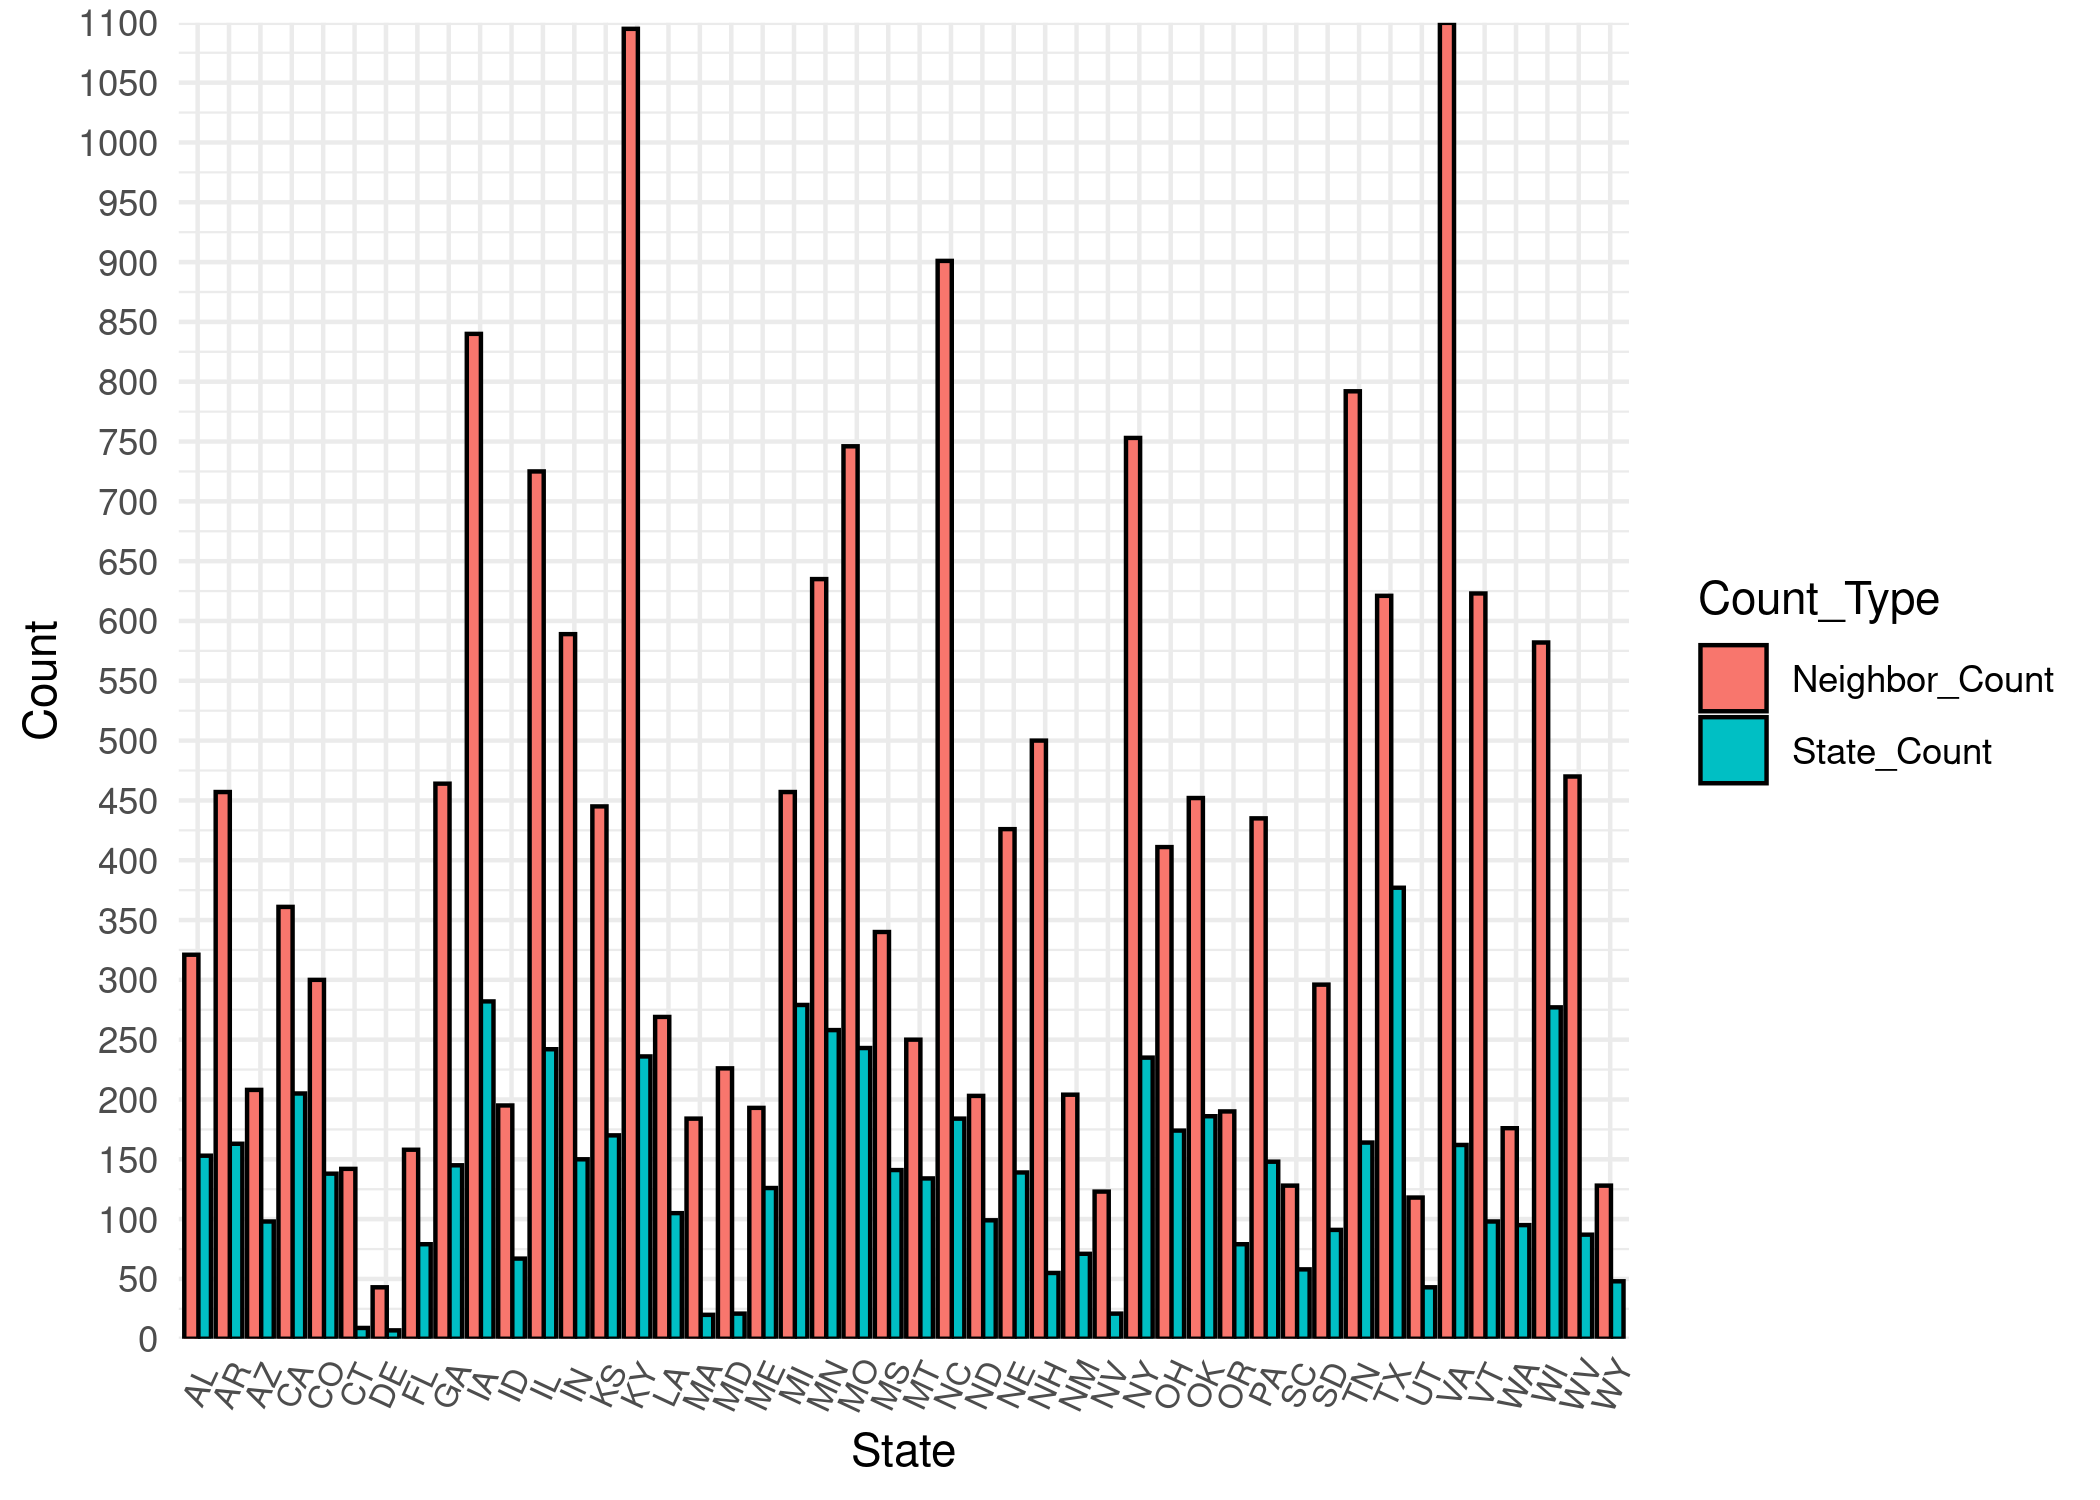
\includegraphics[width=1\textwidth, height=12cm]{plots/neighbors.png}
    \caption{State Census Tracts vs. State Neighbors Count}
    \label{fig:neighbors_bar}
\end{figure}


\section{RUCA Distribution}

Figure~\ref{fig:ruca_frequency} shows the distribution of RUCA codes in the dataset. Small towns with a primary flow within an urban cluster with a population of 2,500 to 9,999 (33 percent) and rural areas with a primary flow to a tract outside an urban area or urban cluster (48 percent) make up the majority of the dataset. The rest are split between small towns with high levels of commuting to a small urban cluster (13 percent) and small towns with low commuting to a small urban cluster  (5 percent). In total, 22.4 million people were considered in the analysis. 

\begin{figure}[htbp]
    \centering
     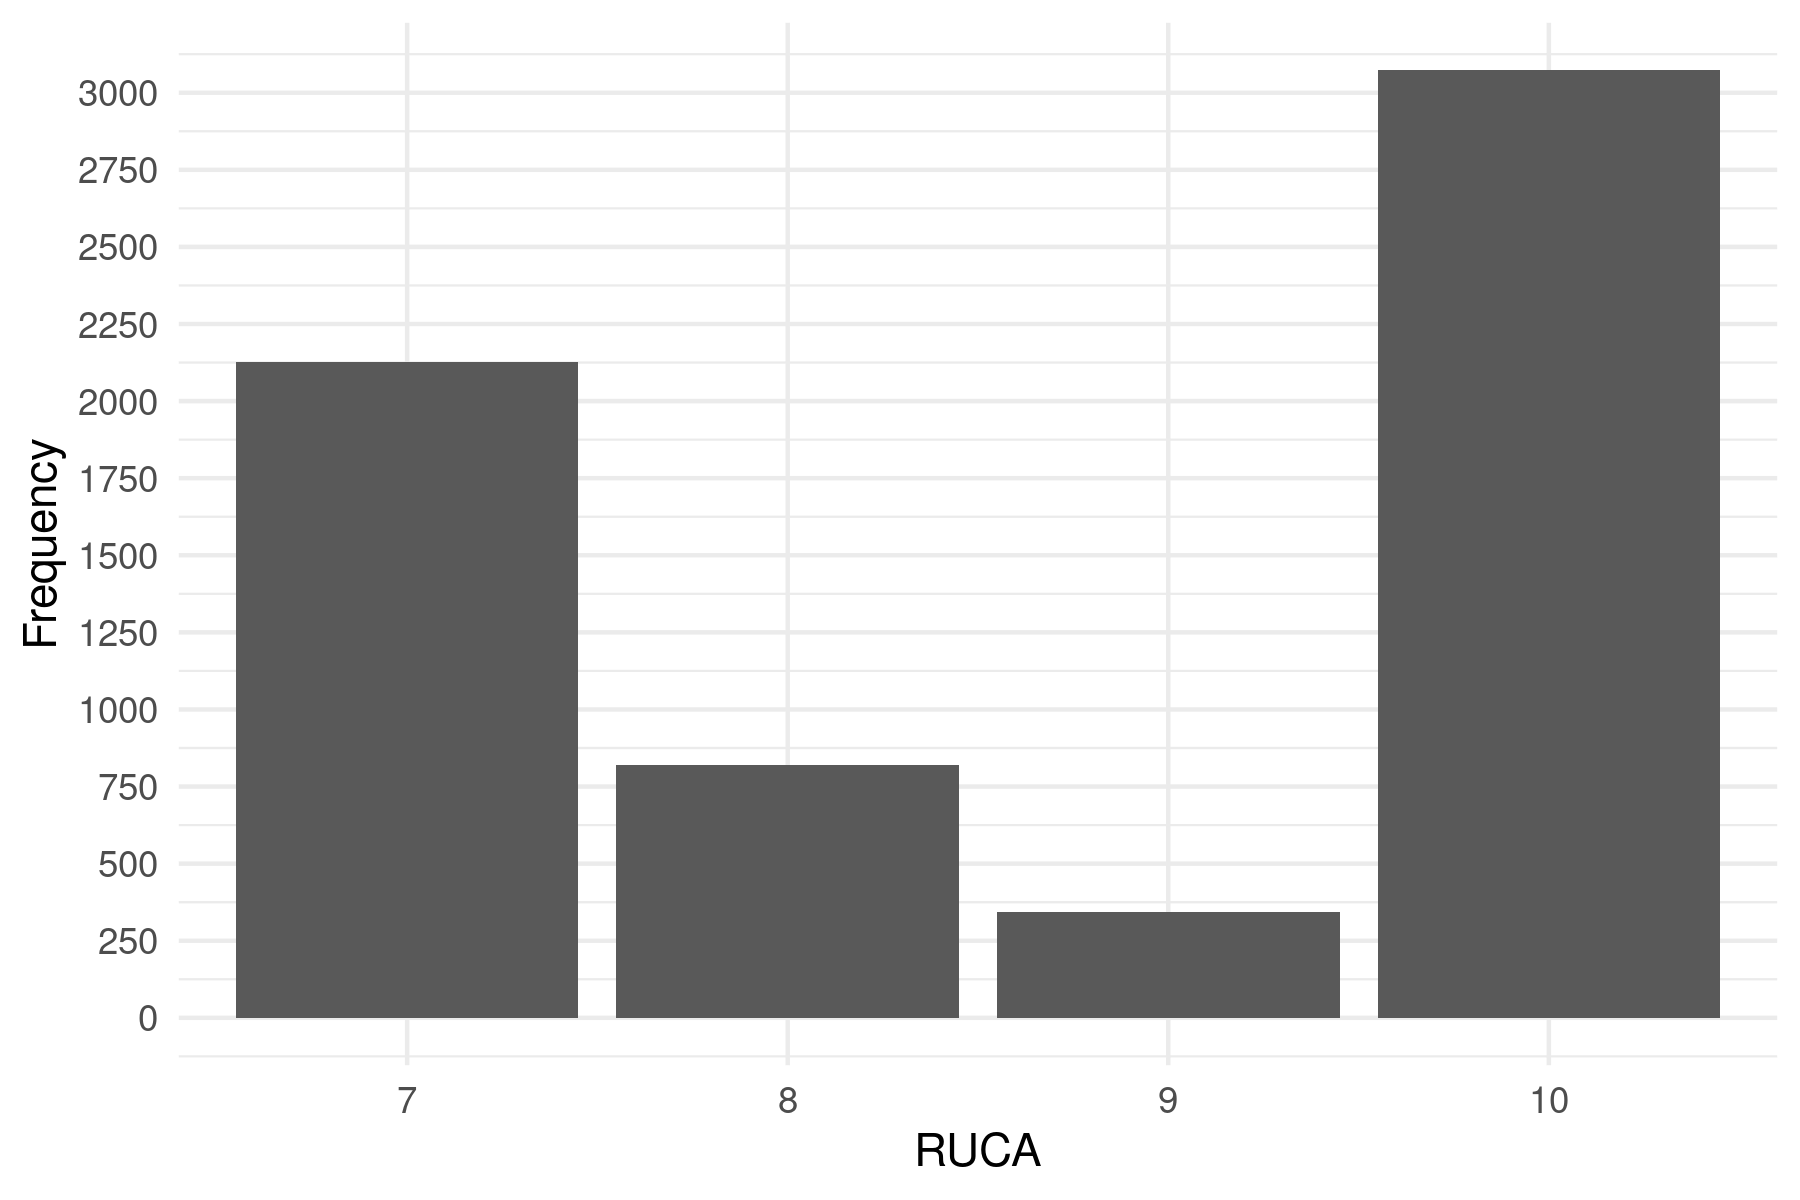
\includegraphics[width=1\textwidth, height=10cm]{plots/ruca_frequency.png}
     \caption{State Census Tracts vs. State Neighbors Count}
     \label{fig:ruca_frequency}
 \end{figure}
 


\section{\textit{Cluster Analysis}}
Here, the results of the cluster analysis are presented for each sector. The primary mechanism for analyzing the clusters is the average cluster medians for all states. The cluster averages were analyzed as well to ensure that the same trends are found in the dataset under a different descriptive statistic. All values are represented as a percentage corresponding to the base unit each sector is scaled to. Figure~\ref{fig:ruca_frequency} shows the distribution of risk levels for each sector. For all sectors except housing cost and demographic diversity, there is a higher number of low-risk rather than high-risk or medium-risk level census tracts. Demographics is the only sector with notably more medium-level than low-level census tracts. 

\begin{figure}[htbp]
    \centering
     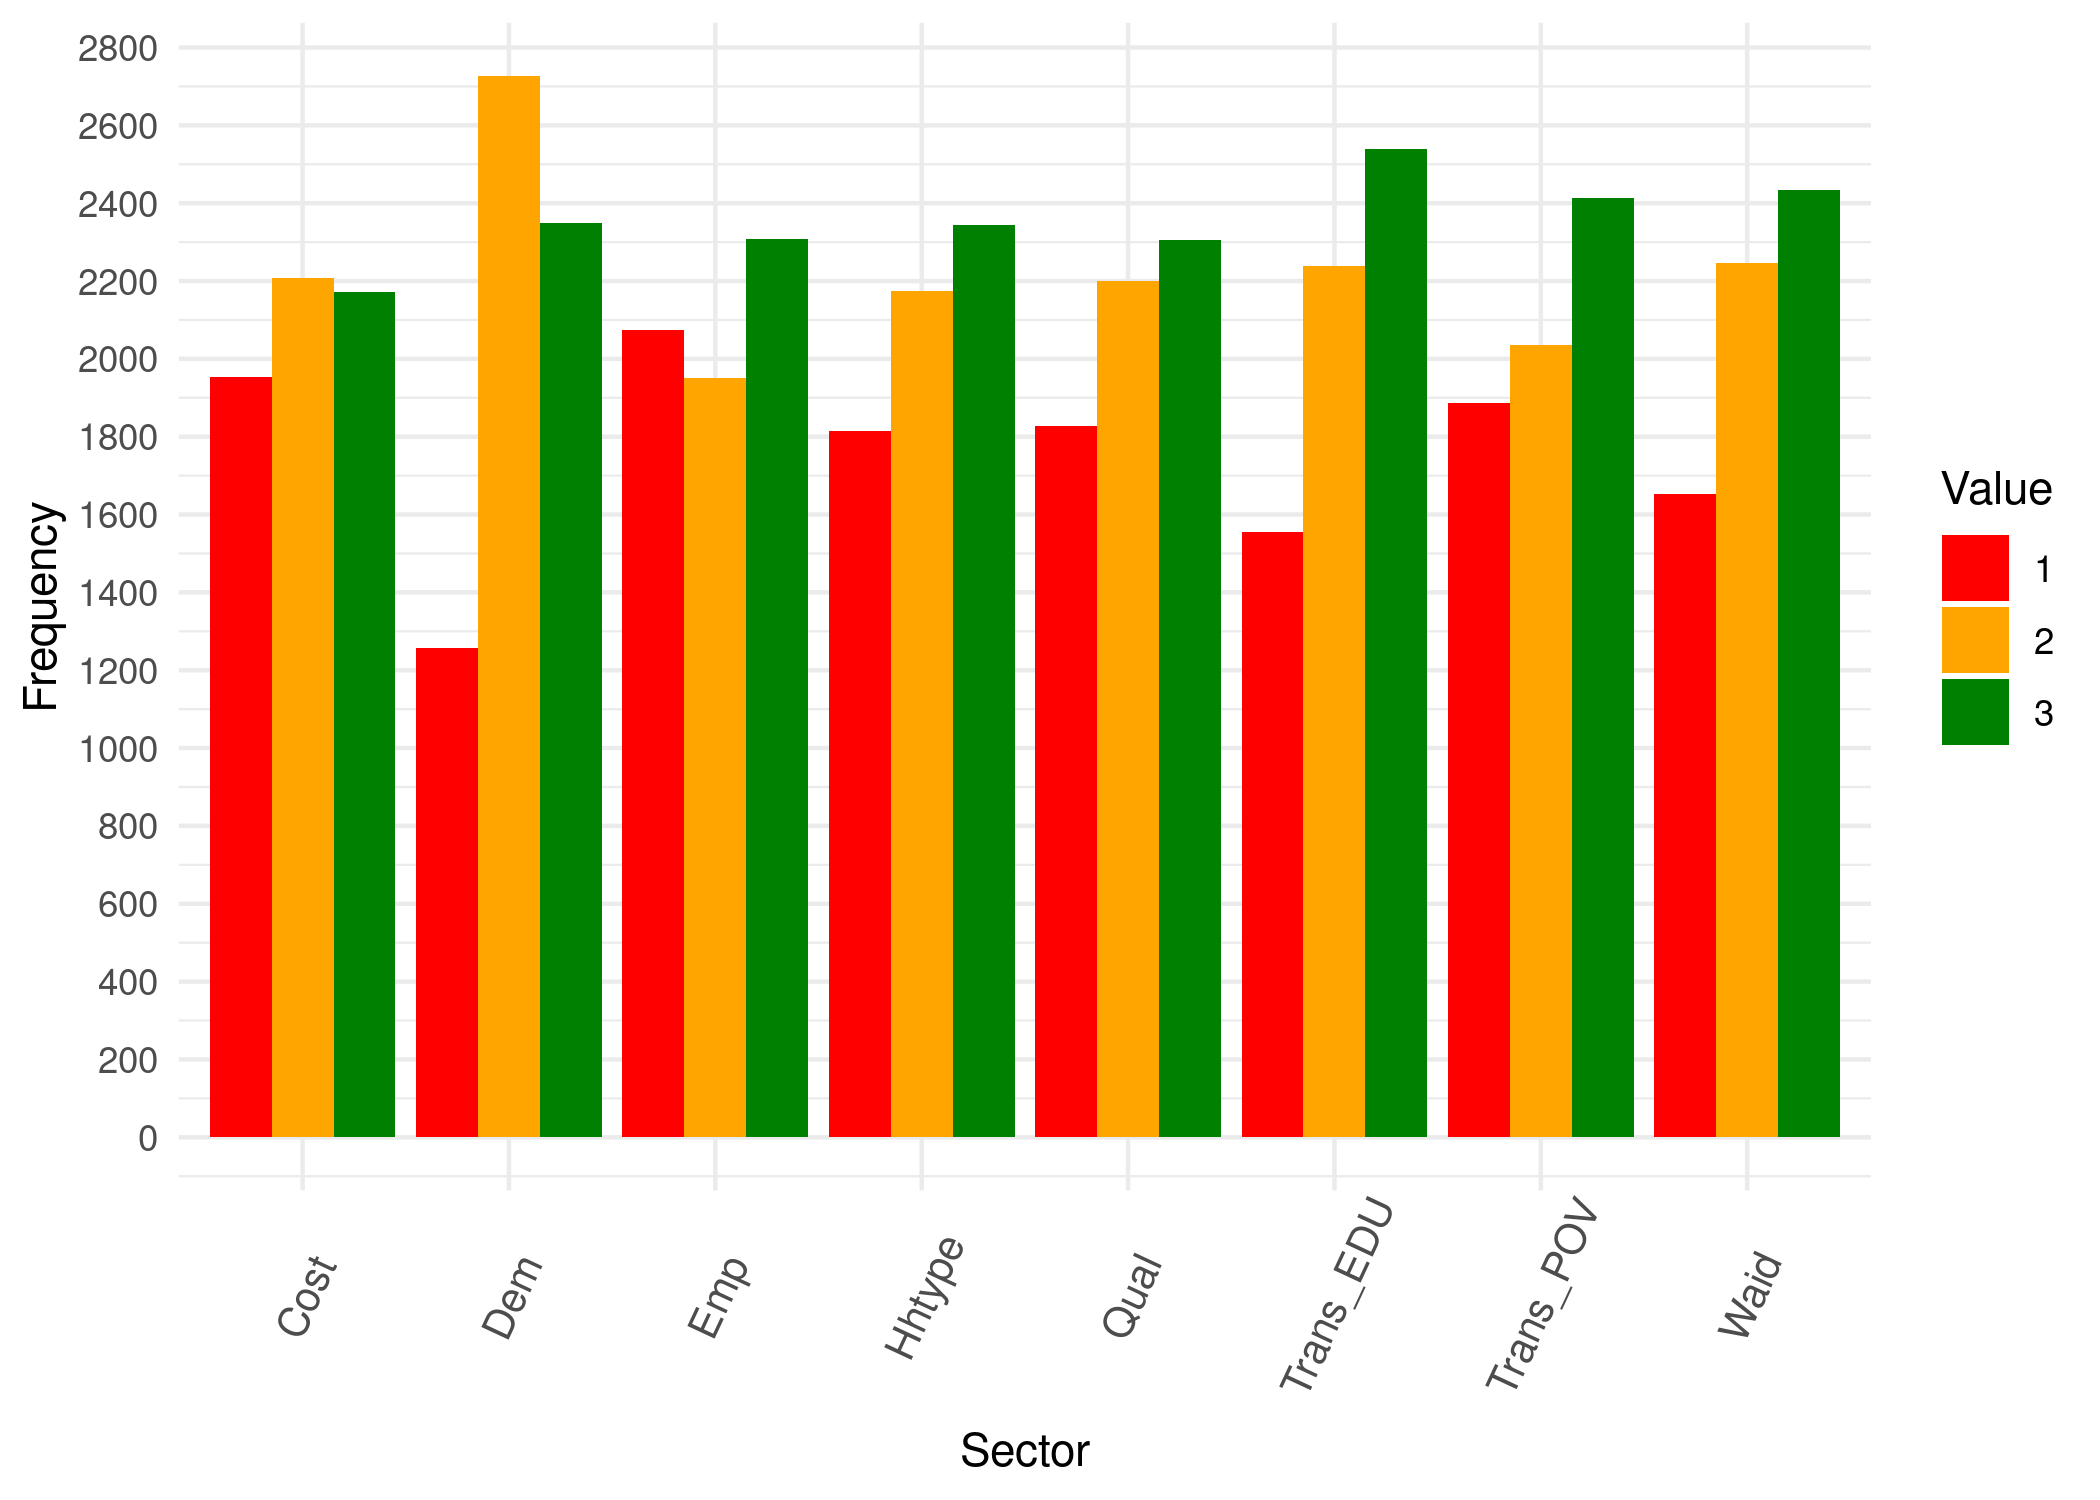
\includegraphics[width=1\textwidth, height=12cm]{plots/cluster_distribution.png}
     \caption{Cluster Distribution by Sector}
     \label{fig:cluster_dis}
 \end{figure}


 
\subsection{\textit{Employment Diversity}}
%The risk levels for employment diversity are determined based on which clusters have the highest number of maximum cluster values compared to the cluster with the lowest number of minimum cluster values. The higher the cluster medians across variables, the better the economic diversity of a cluster. 

Table~\ref{tab:emp} shows that Cluster 1 had the lowest cluster medians in 61 percent of variables, Cluster 2 had the highest cluster median in 53 percent of variables, and Cluster 3 had the middle value in 69 %nice 
percent of cases. Cluster one has the lowest level of economic diversity, Cluster two has the lowest level of economic diversity, and Cluster three has a medium level of economic diversity. Employment in education, health, and social work has the highest presence across each cluster followed by manufacturing. Cluster one becomes the high-risk level, cluster two becomes the low-risk level, and cluster three becomes the medium-risk level.

% latex table generated in R 4.1.2 by xtable 1.8-6 package
% Thu Nov 23 19:11:59 2023
\begin{table}[ht]
    \centering
    \caption{Median Values for Employment Diversity Clusters}
    \label{tab:emp}
    \begin{tabular}{|r| r| r| r|}
        \hline
        Variable & Cluster 1 & Cluster 2 & Cluster 3 \\ 
        \hline
        ag\_for\_fish\_hunt\_mining & 2.54 & 2.24 & 1.87 \\ 
        \hline
        arts\_rec\_food & 2.86 & 3.12 & 3.10 \\ 
        \hline
        construction & 3.16 & 3.06 & 3.07 \\ 
        \hline
        edu\_health\_social & 9.38 & 9.73 & 9.46 \\ 
        \hline
        fin\_re\_insur & 1.47 & 1.60 & 1.57 \\ 
        \hline
        information & 0.35 & 0.41 & 0.37 \\ 
        \hline
        manufacturing & 4.52 & 5.44 & 4.75 \\ 
        \hline
        othersvcs & 1.76 & 1.88 & 1.91 \\ 
        \hline
        prof\_sci\_mgmt\_waste & 2.17 & 2.25 & 2.28 \\ 
        \hline
        public\_admin & 1.98 & 1.88 & 1.92 \\ 
        \hline
        retail\_trade & 4.48 & 4.78 & 4.59 \\ 
        \hline
        trans\_warehouse\_util & 2.17 & 2.03 & 2.12 \\ 
        \hline
        wholesale\_trade & 0.76 & 0.86 & 0.70 \\ 
        \hline
    \end{tabular}
\end{table}



\subsection{\textit{Demographics}}
Due to the historical forces affecting minorities in both rural and urban areas, the risk levels for demographics are based on which clusters have the highest minority populations and the lowest white populations. This sector was decided based on the median and average highest, lowest, and medium value counts as clusters two and three had almost the same cluster median counts.Table~\ref{tab:dem} shows that Cluster three has the middle value for 90 percent of cluster median variables. Cluster three has the highest number of highest values across means and medians with 55 percent of variables. Cluster two is the lowest for 50 percent of variables. Cluster three also has the largest African-American and Hispanic/ Latino cluster medians. Based on this analysis, Cluster one has a medium risk of housing insecurity, Cluster two has a low risk of housing insecurity, and Cluster three has the highest risk of housing insecurity. 

% one notable observation is that the cluster medians for the male/ female over 18 years old variables are roughly three times higher than the male/ female under 18 variables. This reflects the aging population of rural areas noted in the literature. ### move to discussion ###

% latex table generated in R 4.1.2 by xtable 1.8-6 package
% Thu Nov 23 19:33:06 2023
\begin{table}[ht]
    \centering
    \caption{Median Values for Demographic Diversity Clusters}
    \label{tab:dem}
    \begin{tabular}{|r|r|r|r|}
      \hline
     Variable & Cluster 1 & Cluster 2 & Cluster 3 \\ 
      \hline
    am\_in\_ala\_nat & 0.21 & 0.28 & 0.18 \\ 
    \hline
      asian & 0.21 & 0.22 & 0.15 \\ 
      \hline
      black & 0.72 & 0.72 & 0.85 \\ 
      \hline
      female\_o18 & 39.25 & 40.15 & 38.90 \\ 
      \hline
      female\_u18 & 10.77 & 9.79 & 10.98 \\ 
      \hline
      haw\_pac & 0.00 & 0.00 & 0.00 \\ 
      \hline
      hisp\_lat & 2.92 & 2.63 & 3.08 \\ 
      \hline
      male\_o18 & 38.26 & 39.38 & 37.99 \\ 
      \hline
      male\_u18 & 11.44 & 10.27 & 11.70 \\ 
      \hline
      other & 0.32 & 0.30 & 0.41 \\ 
      \hline
      white & 94.35 & 93.67 & 92.52 \\ 
       \hline
    \end{tabular}
    \end{table}

\subsection{\textit{Housing Cost}}

Table~\ref{tab:cost} shows that Cluster 1 has the highest value for mortgage high cost. Cluster two has the lowest mortgage and rent high-cost cluster medians. Cluster three has the highest no-mortgage and rent high-cost cluster medians. Cluster one becomes the medium-risk level, Cluster two becomes the low-risk level, and Cluster three becomes the high-risk level. 

% latex table generated in R 4.1.2 by xtable 1.8-6 package
% Fri Nov 24 09:55:27 2023
\begin{table}[ht]
    \centering
    \caption{Median Values for Housing Cost Clusters}
    \label{tab:cost}
    \begin{tabular}{|r|r|r|r|}
    \hline
    Variable & Cluster 1 & Cluster 2 & Cluster 3 \\ 
    \hline
    mortgage\_high\_cost & 5.22 & 4.35 & 4.93 \\ 
    \hline
      no\_mortgage\_high\_cost & 2.16 & 2.18 & 2.89 \\ 
    \hline
      rent\_high\_cost & 15.69 & 14.18 & 16.79 \\ 
    \hline
    \end{tabular}
    \end{table}

\subsection{\textit{Housing Quality}}
For housing quality, risk levels are determined by which clusters have the highest values, with preference given to occupied housing as housing conditions in unoccupied housing are of lesser concern than occupied housing. Table~\ref{tab:qual} shows that Cluster one has the highest values for unoccupied housing with incomplete kitchens and plumbing. Cluster three has the medium value for each variable. Cluster three has the highest values for occupied housing with incomplete kitchens and plumbing. Cluster one becomes the lowest risk level, cluster two becomes the medium risk level, and cluster three becomes the highest risk level. 

% latex table generated in R 4.1.2 by xtable 1.8-6 package
% Fri Nov 24 09:58:52 2023
\begin{table}[ht]
    \centering
    \caption{Median Values for Housing Quality Clusters}
    \label{tab:qual}
    \begin{tabular}{|r|r|r|r|}
      \hline
     Variable & Cluster 1 & Cluster 2 & Cluster3 \\ 
      \hline
    all\_incomplete\_kitchen & 25.85 & 25.76 & 19.75 \\ 
    \hline
      all\_incomplete\_plumb & 24.00 & 22.73 & 17.28 \\ 
    \hline
      occ\_incomplete\_kitchen & 0.46 & 0.52 & 0.64 \\ 
    \hline
      occ\_incomplete\_plumb & 0.00 & 0.11 & 0.34 \\ 
    \hline
    \end{tabular}
    \end{table}

\subsection{\textit{Residential Mobility: Education}}

For RME, the risk levels are determined by the variables for those who moved with less than a high school education and those in the same house with less than a high school education, and the clusters where more people moved overall will be the highest risk levels. Table~\ref{tab:trans_edu} shows the values for this sector. Cluster one has the medium value for 71 percent of variables including each less than high school education variable. Cluster two has the lowest values for each variable. Cluster 3 has the highest values for 71 percent of variables, including each of the less than high school education variables. Cluster one becomes the lowest risk level because it has medium levels of residential mobility but the highest level of residential stability with a high school education. Cluster two becomes the medium risk level, and cluster three becomes the highest risk level. 

% latex table generated in R 4.1.2 by xtable 1.8-6 package
% Fri Nov 24 10:02:45 2023
\begin{table}[ht]
    \centering
    \caption{Median Values for Residential Mobility: Education Clusters}
    \label{tab:trans_edu}
    \begin{tabular}{|r|r|r|r|}
      \hline
     Variable & Cluster 1 & Cluster 2 & Cluster 3 \\ 
      \hline
    moved\_diff\_county\_hs & 0.51 & 0.44 & 0.55 \\ 
    \hline
      moved\_diff\_county\_less\_than\_hs & 0.13 & 0.10 & 0.18 \\ 
      \hline
      moved\_diff\_state\_hs & 0.18 & 0.10 & 0.18 \\
      \hline 
      moved\_diff\_state\_less\_than\_hs & 0.00 & 0.00 & 0.00 \\
      \hline 
      moved\_in\_county\_hs & 0.95 & 0.84 & 1.36 \\ 
      \hline
      moved\_in\_county\_less\_than\_hs & 0.30 & 0.24 & 0.50 \\ 
      \hline
      same\_house\_hs & 23.99 & 22.60 & 22.97 \\ 
      \hline
      same\_house\_less\_than\_hs & 7.71 & 6.97 & 7.82 \\ 
       \hline
    \end{tabular}
    \end{table}


\subsection{\textit{Residential Mobility: Poverty}}

The RMP sector follows the criteria of residential RME closely with the variables for those who moved that are below the poverty level as the highest priority. Table~\ref{tab:trans_pov} shows that Cluster one has the lowest values for each variable. Cluster two has the medium value for 57 percent of variables. Cluster three has the highest values for 57 percent of variables including three of the below the poverty level variables. Cluster one becomes the lowest risk level, cluster two becomes the medium risk level, and cluster three becomes the highest risk level. 

% RMP: one noteable observation from the cluster medians is that cluster three has the highest value of those living in the same house below and above the poverty measure, indicating high levels of poverty for census tracts in this cluster. ### move to discussion ###

% latex table generated in R 4.1.2 by xtable 1.8-6 package
% Fri Nov 24 10:09:00 2023
\begin{table}[ht]
    \centering
    \caption{Median Values for Residential Mobility: Poverty Clusters}
    \label{tab:trans_pov}
    \begin{tabular}{|r|r|r|r|}
      \hline
     & cluster\_1 & cluster\_2 & cluster\_3 \\ 
      \hline
    moved\_diff\_county\_p1 & 0.30 & 0.41 & 0.48 \\
    \hline 
      moved\_diff\_county\_p2 & 0.04 & 0.12 & 0.07 \\ 
      \hline
      moved\_diff\_state\_p1 & 0.05 & 0.10 & 0.08 \\ 
      \hline
      moved\_diff\_state\_p2 & 0.00 & 0.00 & 0.00 \\ 
      \hline
      moved\_in\_county\_p1 & 0.74 & 1.00 & 1.06 \\ 
      \hline
      moved\_in\_county\_p2 & 0.30 & 0.43 & 0.40 \\ 
      \hline
      same\_house\_p1 & 9.86 & 10.80 & 12.14 \\ 
      \hline
      same\_house\_p2 & 7.79 & 8.55 & 9.04 \\ 
       \hline
    \end{tabular}
    \end{table}

\subsection{\textit{Wage and Household Factors}}

For household wage/ aid, the clusters with the highest number of maximum cluster medians determine the risk levels with particular attention given to households with no wage and households with three or more workers Table~\ref{tab:waid} shows the values for this sector. Cluster one has the lowest cluster medians for 89 percent of variables. Cluster two has the medium value for 55 percent of variables. Cluster three has the highest values for 55 percent of variables and the middle value for the other variables. Notable high values for cluster three include the Gini index, households with no vehicle, households with at least one worker and no vehicle, and households receiving supplemental security income.  

% latex table generated in R 4.1.2 by xtable 1.8-6 package
% Fri Nov 24 10:25:00 2023
\begin{table}[ht]
    \centering
    \caption{Median Values for Household Factor Clusters}
    \label{tab:waid}
    \begin{tabular}{|r|r|r|r|}
      \hline
     & Cluster 1 & Cluster 2 & Cluster 3 \\ 
      \hline
    gini\_index & 42.69 & 42.91 & 44.07 \\ 
    \hline
      hh\_3plus\_worker & 1.85 & 1.67 & 1.81 \\ 
      \hline
      hh\_no\_investment\_income & 32.64 & 33.04 & 33.29 \\ 
      \hline
      hh\_no\_other\_income & 36.28 & 36.81 & 36.79 \\ 
      \hline
      hh\_no\_vehicle & 1.96 & 2.12 & 2.34 \\ 
      \hline
      hh\_no\_wage & 13.38 & 14.11 & 14.01 \\ 
      \hline
      hh\_public\_assistance & 4.84 & 5.54 & 5.40 \\ 
      \hline
      hh\_ssi & 2.17 & 2.39 & 2.51 \\ 
      \hline
      hh\_worker\_no\_vehicle & 1.28 & 1.45 & 1.59 \\ 
       \hline
    \end{tabular}
    \end{table}

\subsection{\textit{Housing Type}}
For the housing type sector, owner single unit is considered the safest housing while renters and owners of unconventional housing and mobile homes are considered high risk. This sector required a combination of means and medians for the analysis because, for several variables, all cluster medians are zero. Table~\ref{tab:hh_type} shows the values for this sector. Cluster three has the highest owner mobile and the medium value for renter mobile. Cluster three has the highest renter and owner unconventional cluster averages. Cluster one has the highest owner single and the lowest renter mobile home. Cluster one becomes the low-risk level, cluster two becomes the medium-risk level, and Cluster Three becomes the high-risk level.

% latex table generated in R 4.1.2 by xtable 1.8-6 package
% Fri Nov 24 10:28:27 2023
\begin{table}[ht]
    \centering
    \caption{Median Values for Housing Type Clusters}
    \label{tab:hh_type}
    \begin{tabular}{|r|r|r|r|}
      \hline
     Variable & Cluster 1 & Cluster 2 & Cluster 3 \\ 
      \hline
    owner\_2to4 & 0.00 & 0.00 & 0.00 \\ 
    \hline
      owner\_5plus & 0.00 & 0.00 & 0.00 \\ 
      \hline
      owner\_mobile & 8.29 & 10.06 & 10.41 \\ 
      \hline
      owner\_single & 90.75 & 88.67 & 88.42 \\ 
      \hline
      owner\_unconvent & 0.00 & 0.00 & 0.00 \\
      \hline 
      renter\_2to4 & 8.29 & 10.57 & 10.59 \\ 
      \hline
      renter\_5plus & 5.78 & 8.50 & 7.70 \\ 
      \hline
      renter\_mobile & 9.25 & 13.04 & 10.79 \\ 
      \hline
      renter\_single & 68.16 & 55.67 & 60.95 \\ 
      \hline
      renter\_unconvent & 0.00 & 0.00 & 0.00 \\ 
       \hline
    \end{tabular}
    \end{table}


\section{\textit{Association Rules}}

There are three areas of investigation for the association rules generated from the housing insecurity risk levels. First are high-risk-to-high-risk associations (1:1), second are low-risk-to-low-risk associations (3:3), third are inverse relationships: low-risk-to-high-risk associations (3:1) and high-risk-to-low-risk associations (1:3). Tables~\ref{tab:high_risk_ass},~\ref{tab:low_risk_ass},~\ref{tab:low_high_risk}, and~\ref{tab:high_low_risk} show the average support, average confidence, coverage, and average lift for the different association rules. Figure~\ref{fig:assoc_scatter} shows the overall trends in the association rules. Support is low with confidence below 0.2 for most of the rules.  There are 23 rules with support greater than 0.2 that reflect the occurrence of each risk level for each sector. The plot shows a notable amount of clustering around the 0.35 confidence and 0.1 support range. For each set of association rules, their average lift values indicate that the likelihood of finding the items together is only slightly more or slightly less than their likelihood of being found together by chance. The high-risk-to-high-risk associations have the lowest average support values of the four groups of rules, and low-risk-to-low-risk associations have the highest average support. All average confidence values range from 0.2 to 0.4, indicating that for the risk level on the left-hand side of the transaction, there is an average 20 to 40 percent probability of each other risk level being on the right-hand side of the transaction. Overall, the association rules indicate that there is little consistency in census tracts showing signs of housing insecurity risk at different levels. 


 \begin{figure}[htbp]
    \centering
     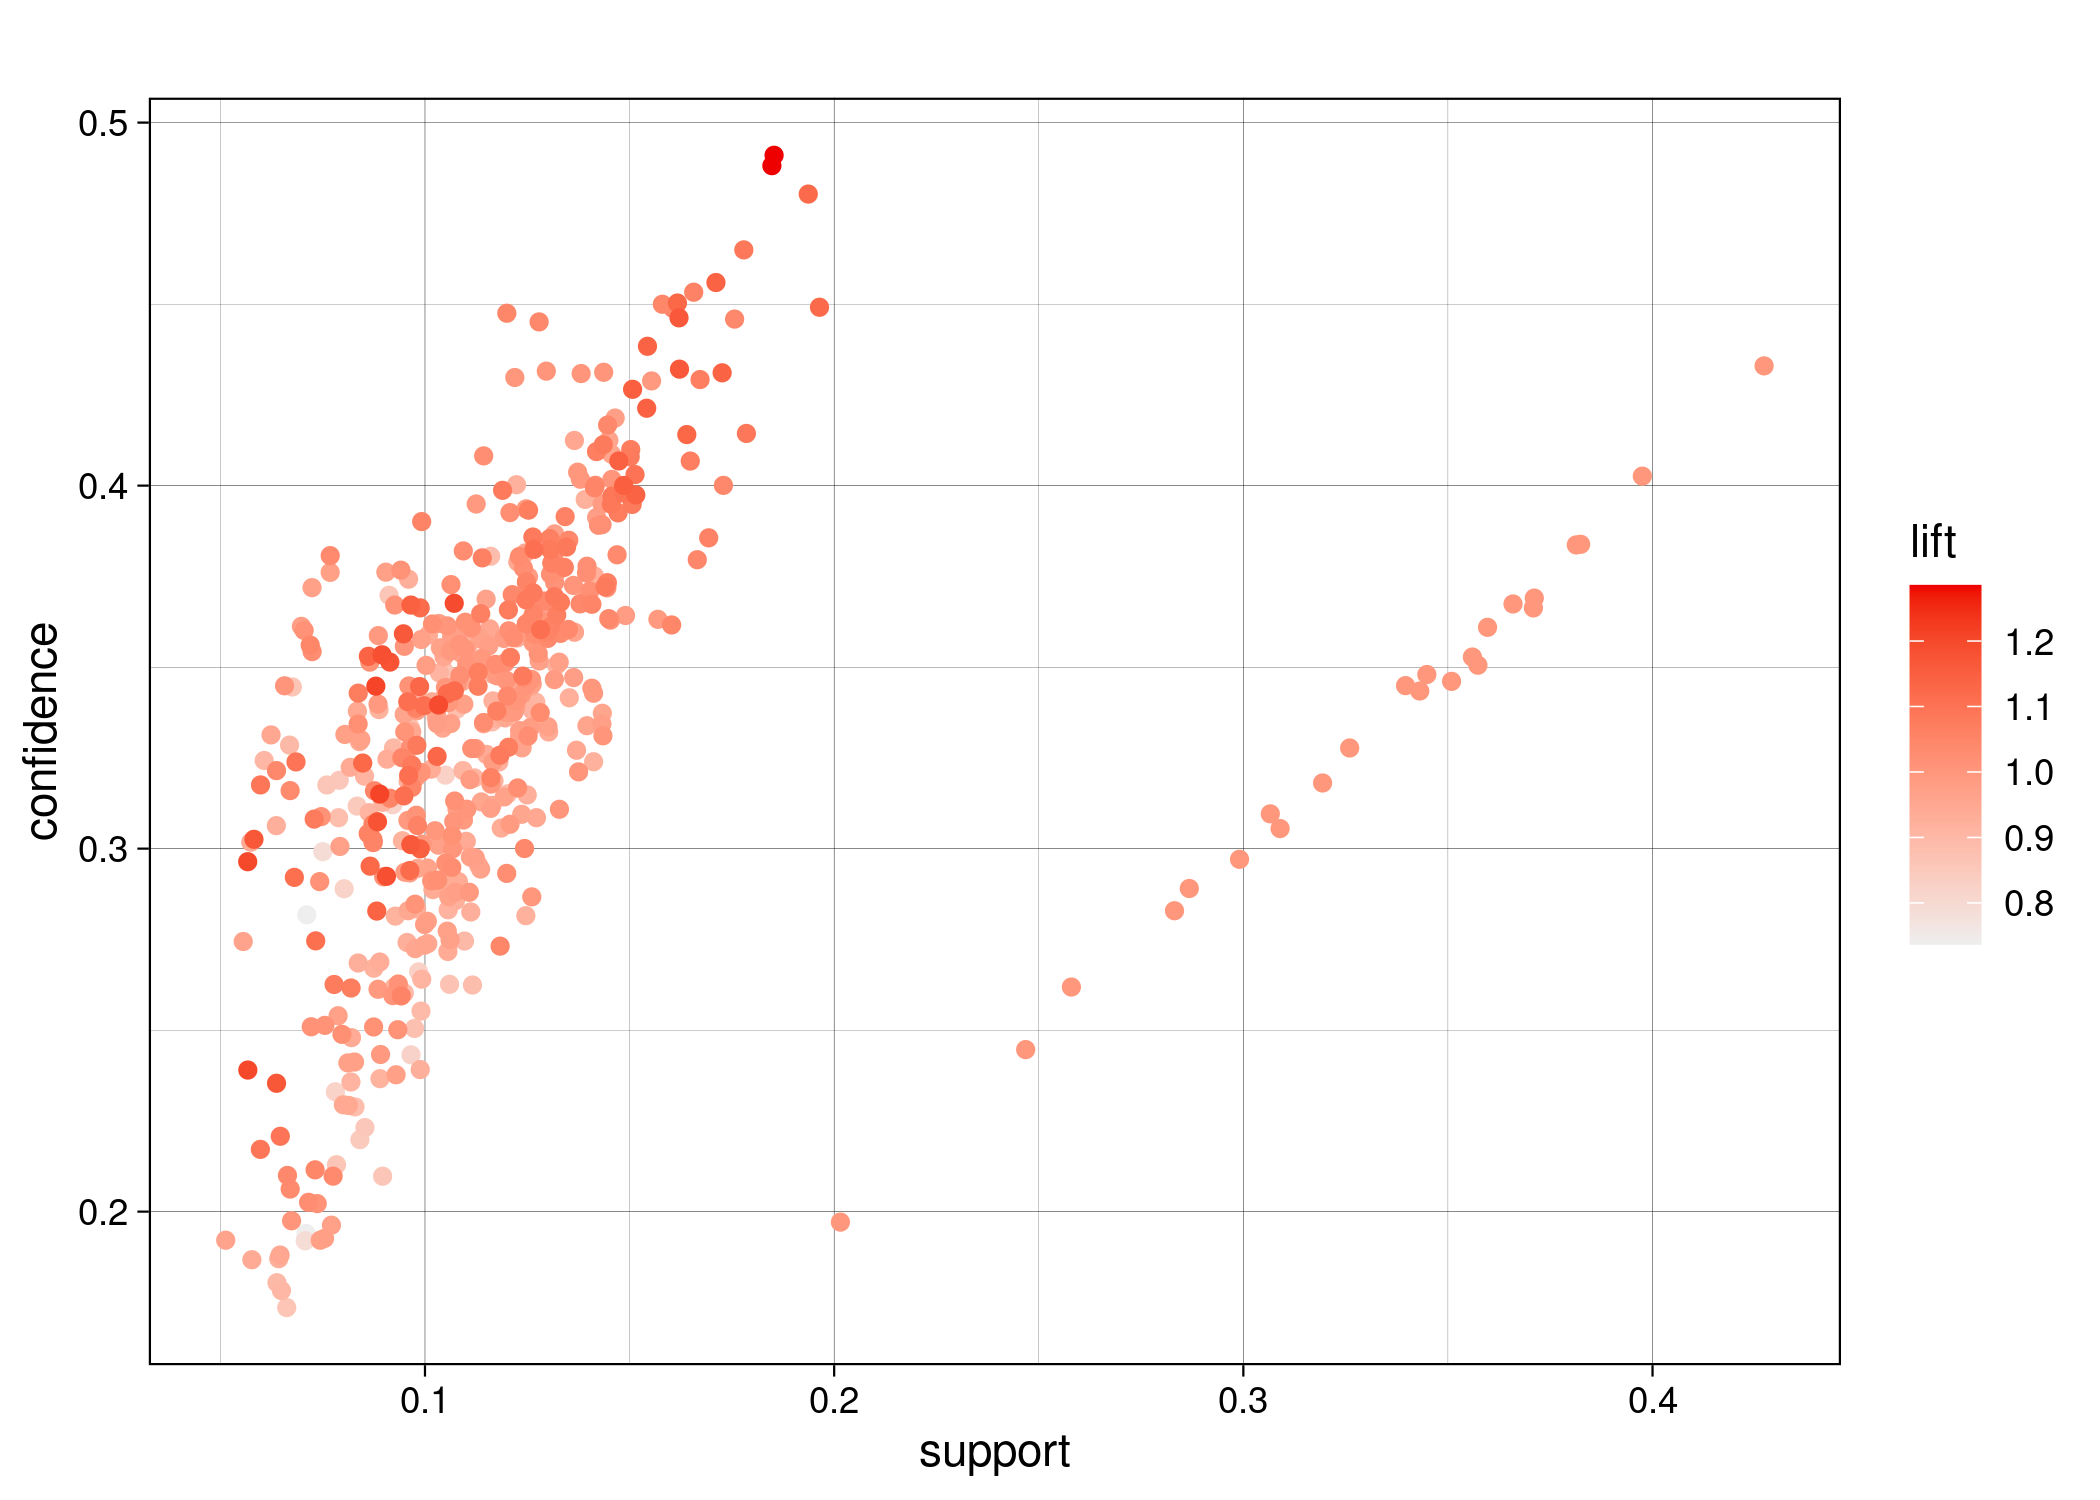
\includegraphics[width=1\textwidth, height=10cm]{plots/assoc_scatter.png}
     \caption{Scatter plot of Association Rules Statistics}
     \label{fig:assoc_scatter} % filter out empty left hand side rules (support > 0.2)
 \end{figure}

\begin{table}[h]
    \centering
    \caption{High Risk Association Average Statistics}
    \label{tab:high_risk_ass} % Correct placement of label
    \begin{tabular}{|c|c|c|c|c|}
    \hline
    Sector & Average Support & Average Confidence & Average Coverage & Average Lift \\
    \hline
    employment & 0.09 & 0.27 & 0.33 & 0.99 \\
    demographics & 0.06 & 0.31 & 0.2 & 1.1 \\
    rm: education & 0.07 & 0.3 & 0.25 & 1.1 \\
    rm: poverty & 0.09 & 0.3 & 0.3 & 1.1 \\
    cost & 0.09 & 0.29 & 0.31 & 1.1 \\
    qual & 0.08 & 0.29 & 0.29 & 1.1 \\
    housing type & 0.08 & 0.3 & 0.29 & 1.1 \\
    household factors & 0.08 & 0.32 & 0.26 & 1.2 \\
    \hline
    \end{tabular}
\end{table}

\begin{table}[h]
    \centering
    \caption{Low Risk Association Average Statistics}
    \label{tab:low_risk_ass} % Correct placement of label
    \begin{tabular}{|c|c|c|c|c|}
    \hline
    Sector & Average Support & Average Confidence & Average Coverage & Average Lift \\
    \hline
    employment & 0.14 & 0.39 & 0.37 & 1.00 \\
    demographics & 0.13 & 0.36 & 0.37 & 1 \\
    rm: education & 0.15 & 0.38 & 0.4 & 1 \\
    rm: poverty & 0.15 & 0.4 & 0.38 & 1.1 \\
    cost & 0.13 & 0.37 & 0.34 & 1 \\
    qual & 0.14 & 0.38 & 0.36 & 1 \\
    housing type & 0.14 & 0.39 & 0.37 & 1 \\
    household factors & 0.15 & 0.4 & 0.38 & 1.1 \\
    \hline
    \end{tabular}
\end{table}

\begin{table}[h]
    \centering
    \caption{Low to High Risk Association Average Statistics}
    \label{tab:low_high_risk}
    \begin{tabular}{|c|c|c|c|c|}
    \hline
    Sector & Average Support & Average Confidence & Average Coverage & Average Lift \\
    \hline
    employment & 0.09 & 0.25 & 0.37 & 0.95 \\
    \hline
    demographics & 0.11 & 0.28 & 0.37 & 0.99 \\
    \hline
    rm: education & 0.11 & 0.27 & 0.4 & 0.95 \\
    \hline
    rm: poverty & 0.09 & 0.24 & 0.38 & 0.89 \\
    \hline
    cost & 0.09 & 0.27 & 0.34 & 0.99 \\
    \hline
    qual & 0.1 & 0.27 & 0.36 & 0.97 \\
    \hline
    housing type & 0.1 & 0.26 & 0.37 & 0.96 \\
    \hline
    household factors & 0.1 & 0.25 & 0.38 & 0.91 \\
    \hline
    \end{tabular}

    \end{table}

\begin{table}[h]
    \centering
    \caption{High to Low Risk Association Average Statistics}
    \label{tab:high_low_risk}
    \begin{tabular}{|c|c|c|c|c|}
    \hline
    Sector & Average Support & Average Confidence & Average Coverage & Average Lift \\
    \hline
    employment & 0.12 & 0.37 & 0.33 & 0.98 \\
    \hline
    demographics & 0.7 & 0.36 & 0.2 & 0.96 \\
    \hline
    rm: education & 0.09 & 0.35 & 0.25 & 0.95 \\
    \hline
    rm: poverty & 0.11 & 0.35 & 0.3 & 0.96 \\
    \hline
    cost & 0.11 & 0.36 & 0.31 & 0.94 \\
    \hline
    qual & 0.1 & 0.36 & 0.19 & 0.95 \\
    \hline
    housing type & 0.1 & 0.36 & 0.29 & 0.96 \\
    \hline
    household factors & 0.09 & 0.33 & 0.26 & 0.89 \\
    \hline
    \end{tabular}
    \end{table}
      

\section{\textit{Moran's I}}

While the association rules dealt exclusively with the housing insecurity risk levels, Moran’s I spatial autocorrelation is used to examine how values group in space for the variables and risk levels. Moran’s I is calculated for every state and the entire dataset.  Table~\ref{moran_desc} shows the descriptive statistics for the significant Moran's I values
Table~\ref{moran_sector} shows the average of statistically significant Moran's I values across sectors. Variable averages show similar trends as the sector averages. Manufacturing has the highest average Moran's I statistic at 0.43, followed by white at 0.38 and ag-for-fish-hunt-mining at 0.34. There is a weak spatial autocorrelation between the different levels of rurality at 0.29. The sector averages are low, ranging from 0.19 to 0.32. While averages are low, certain observations deserve further attention. Nationally, there are 7 variables with notable statistically significant Moran's I values. These include the white population (0.66), American Indian and Native Alaskan (0.61), the catch-all ag\_for\_fish\_hunt\_mining variable (0.61), owners of mobile homes (0.56), individuals living in the same house with less than a high school education (0.57), owners of single-unit homes (0.55) and the "other" demographic variable (0.54). Two crucial variables, renters and owners of unconventional housing show almost no spatial autocorrelation at 0.04 and 0.08 respectively. Most of the variables with average Moran's I scores less than 0.1 are in the residential mobility sectors. The nationwide global spatial autocorrelation scores for the sector variables range from low (0.17) to a medium strength spatial autocorrelation (0.35) with demographic risk levels being the most spatially clustered and housing costs being the least spatially clustered.

\begin{table}[!htbp] \centering 
    \caption{Moran's I Descriptive Statistics} 
    \label{moran_desc} 
  \begin{tabular}{@{\extracolsep{5pt}}lccccc} 
  \\[-1.8ex]\hline 
  \hline \\[-1.8ex] 
  Statistic & \multicolumn{1}{c}{N} & \multicolumn{1}{c}{Mean} & \multicolumn{1}{c}{St. Dev.} & \multicolumn{1}{c}{Min} & \multicolumn{1}{c}{Max} \\ 
  \hline \\[-1.8ex] 
  N & 2,018 & 445.284 & 1,153.592 & 12 & 6,333 \\ 
  Morans\_I & 2,018 & 0.259 & 0.141 & 0.014 & 0.935 \\ 
  std\_dev & 2,018 & 5.451 & 6.023 & 1.646 & 72.172 \\ 
  variance & 2,018 & 0.004 & 0.005 & 0.00001 & 0.083 \\ 
  expectation & 2,018 & $-$0.006 & 0.007 & $-$0.091 & $-$0.0002 \\ 
  p\_value & 2,018 & 0.005 & 0.011 & 0.000 & 0.050 \\ 
  \hline \\[-1.8ex] 
  \end{tabular} 
  \end{table} 

\begin{table}[ht]
    \centering
    \begin{tabular}{lrrrrr}
      \hline
    sector & Morans\_I & std\_dev & variance & expectation & p\_value \\ 
      \hline
    Demographics & 0.32 & 7.02 & 0.00 & -0.01 & 0.00 \\ 
      Employment & 0.25 & 5.38 & 0.00 & -0.01 & 0.01 \\ 
      Household Wage/ Aid & 0.26 & 5.23 & 0.00 & -0.01 & 0.00 \\ 
      Housing Cost & 0.21 & 4.43 & 0.00 & -0.01 & 0.01 \\ 
      Housing Quality & 0.28 & 5.59 & 0.00 & -0.01 & 0.00 \\ 
      Housing Type & 0.25 & 5.32 & 0.00 & -0.01 & 0.01 \\ 
      RUCA & 0.31 & 5.86 & 0.00 & -0.01 & 0.00 \\ 
      Transience: Education & 0.23 & 4.77 & 0.00 & -0.01 & 0.01 \\ 
      Transience: Poverty & 0.19 & 4.11 & 0.00 & -0.01 & 0.01 \\ 
       \hline
    \end{tabular}
    \end{table}


%% latex table generated in R 4.1.2 by xtable 1.8-6 package
% Fri Nov 24 19:26:09 2023
\begin{longtable}{|c|c|c|}
    \caption{Moran's I Values for All Census Tracts} \label{tab:all_mi} \\
    \hline
    \textbf{Sector} & \textbf{Variable Name} & \textbf{Moran's I} \\
    \hline
    \endfirsthead
    
    \multicolumn{3}{c}%
    {{\tablename\ \thetable{} -- continued from previous page}} \\
    \hline
    \textbf{Sector} & \textbf{Variable Name} & \textbf{Moran's I} \\
    \hline
    \endhead
    
    \hline \multicolumn{3}{r}{{Continued on next page}} \\
    \endfoot
    
    \hline
    \endlastfoot
    
    RUCA & RUCA & 0.33 *** \\ 
    Employment Diversity & ag\_for\_fish\_hunt\_mining & 0.61 *** \\ 
     & construction & 0.24 *** \\ 
     & manufacturing & 0.71 *** \\ 
     & wholesale\_trade & 0.32 *** \\ 
     & retail\_trade & 0.17 *** \\ 
     & trans\_warehouse\_util & 0.21 *** \\ 
     & information & 0.13 *** \\ 
     & fin\_re\_insur & 0.25 *** \\ 
     & prof\_sci\_mgmt\_waste & 0.48 *** \\ 
     & edu\_health\_social & 0.36 *** \\ 
     & arts\_rec\_food & 0.38 *** \\ 
     & othersvcs & 0.1 *** \\ 
     & public\_admin & 0.28 *** \\ 
     & Emp\_Cluster & 0.2 *** \\ 
    Demographics & white & 0.66 *** \\ 
     & black & 0.74 *** \\ 
     & am\_in\_ala\_nat & 0.61 *** \\ 
     & asian & 0.2 *** \\ 
     & haw\_pac & 0.07 *** \\ 
     & other & 0.54 *** \\ 
     & hisp\_lat & 0.71 *** \\ 
     & male\_u18 & 0.24 *** \\ 
     & female\_u18 & 0.24 *** \\ 
     & male\_o18 & 0.11 *** \\ 
     & female\_o18 & 0.19 *** \\ 
     & Dem\_Cluster & 0.35 *** \\ 
    Residential Mobility: Education & same\_house\_less\_than\_hs & 0.57 *** \\ 
     & same\_house\_hs & 0.47 *** \\ 
     & moved\_in\_county\_less\_than\_hs & 0.14 *** \\ 
     & moved\_in\_county\_hs & 0.1 *** \\ 
     & moved\_diff\_county\_less\_than\_hs & 0.08 *** \\ 
     & moved\_diff\_county\_hs & 0.09 *** \\ 
     & moved\_diff\_state\_less\_than\_hs & 0.03 ** \\ 
     & moved\_diff\_state\_hs & 0.1 *** \\ 
     & Trans\_EDU\_Cluster & 0.15 *** \\ 
    Residential Mobility: Poverty & same\_house\_p1 & 0.43 *** \\ 
     & same\_house\_p2 & 0.21 *** \\ 
     & moved\_in\_county\_p1 & 0.12 *** \\ 
     & moved\_in\_county\_p2 & 0.05 *** \\ 
     & moved\_diff\_county\_p1 & 0.05 *** \\ 
     & moved\_diff\_county\_p2 & 0.01  \\ 
     & moved\_diff\_state\_p1 & 0.06 *** \\ 
     & moved\_diff\_state\_p2 & 0.03 ** \\ 
     & Trans\_POV\_Cluster & 0.17 *** \\ 
    Housing Type & owner\_single & 0.55 *** \\ 
     & owner\_2to4 & 0.23 *** \\ 
     & owner\_5plus & 0.14 *** \\ 
     & owner\_mobile & 0.57 *** \\ 
     & owner\_unconvent & 0.08 *** \\ 
     & renter\_single & 0.24 *** \\ 
     & renter\_2to4 & 0.19 *** \\ 
     & renter\_5plus & 0.13 *** \\ 
     & renter\_mobile & 0.33 *** \\ 
     & renter\_unconvent & 0.04 *** \\ 
     & Hhtype\_Cluster & 0.16 *** \\ 
    Housing Cost & mortgage\_high\_cost & 0.44 *** \\ 
     & no\_mortgage\_high\_cost & 0.15 *** \\ 
     & rent\_high\_cost & 0.13 *** \\ 
     & Cost\_Cluster & 0.12 *** \\ 
    Household Factors & hh\_no\_wage & 0.44 *** \\ 
     & hh\_no\_other\_income & 0.35 *** \\ 
     & hh\_no\_investment\_income & 0.37 *** \\ 
     & hh\_public\_assistance & 0.43 *** \\ 
     & hh\_ssi & 0.39 *** \\ 
     & hh\_3plus\_worker & 0.26 *** \\ 
     & hh\_worker\_no\_vehicle & 0.19 *** \\ 
     & hh\_no\_vehicle & 0.2 *** \\ 
     & gini\_index & 0.23 *** \\ 
     & Waid\_Cluster & 0.18 *** \\ 
    Housing Quality & all\_incomplete\_plumb & 0.24 *** \\ 
     & all\_incomplete\_kitchen & 0.3 *** \\ 
     & occ\_incomplete\_plumb & 0.47 *** \\ 
     & occ\_incomplete\_kitchen & 0.3 *** \\ 
     & Qual\_Cluster & 0.2 *** \\ 
       \hline
    \textbf{Significance} & \multicolumn{2}{c|}{* $p < 0.05$, ** $p < 0.01$, *** $p < 0.001$} \\
\end{longtable}


\subsection{Moran's I Outliers}
% TODO: rewrite intro sentence
Outliers based on the interquartile range (IRQ) method are calculated for the calculated Moran's I statistics to highlight areas that do not follow the overall trends in the data set. There are 134 statistically significant Moran's I values greater than 0.5 not including the nationwide calculations. These observations are spread across 38 states, with Arizona and New Mexico accounting for 16 percent of high Moran's I statistics. Figure~\ref{fig:moran_sector} shows the distribution of Moran's I for each sector. Demographics and household factors do not have any outliers based on the IRQ method. RMP has 13 outliers. The mean of all RMP observations is 0.19 while the mean for the outliers is 0.47. 69 percent of these outliers are the same house below the poverty line variable. Connecticut, Nevada, and Arizona have surprisingly high Moran’s I statistics for the RMP risk levels variable. The average for these three states is 0.45 compared to 0.21 for the same variable overall. There are 4 outliers in the residential RME sector with same\_house\_less\_than\_hs in Ohio, California, and all states. The final outlier is same\_house\_hs in Maryland. These outliers have an average of 0.61 while all sector observations have an average of 0.23. For housing type, there are two outliers: owner\_single and owner\_mobile, both in South Dakota. These outliers have an average Moran’s I of 0.63 while the sector has an average of 0.25. For housing quality there are two outliers: occupied incomplete plumbing and occupied incomplete kitchen, both in the state of New Mexico. The sector average is 0.28 while these outliers have an average of 0.66. Housing cost has six outliers: mortgage high cost in Arizona, Maryland, Minnesota, Nevada, and New Mexico. The variable average is 0.28 while these observations have an average of 0.5. For economic diversity, there are 16 outliers, 10 of these observations are for manufacturing nationally and in Virginia, Florida, Indiana, Kentucky, Mississippi, Ohio, Pennsylvania, South Dakota, and Virginia. The average Moran’s I statistic for this sector was 0.47 while these outliers have an average of 0.68. five of these outliers are for the agriculture, forestry, fishing, hunting, and mining variable in New Mexico, Oklahoma, Texas, Washington, and nationally. The average Moran’s I statistic for this variable is 0.36 while these outliers have an average of 0.61. Figure~\ref{fig:moran_region} shows the distribution of Moran's I for each state by region.

\begin{figure}[htbp]
    \centering
     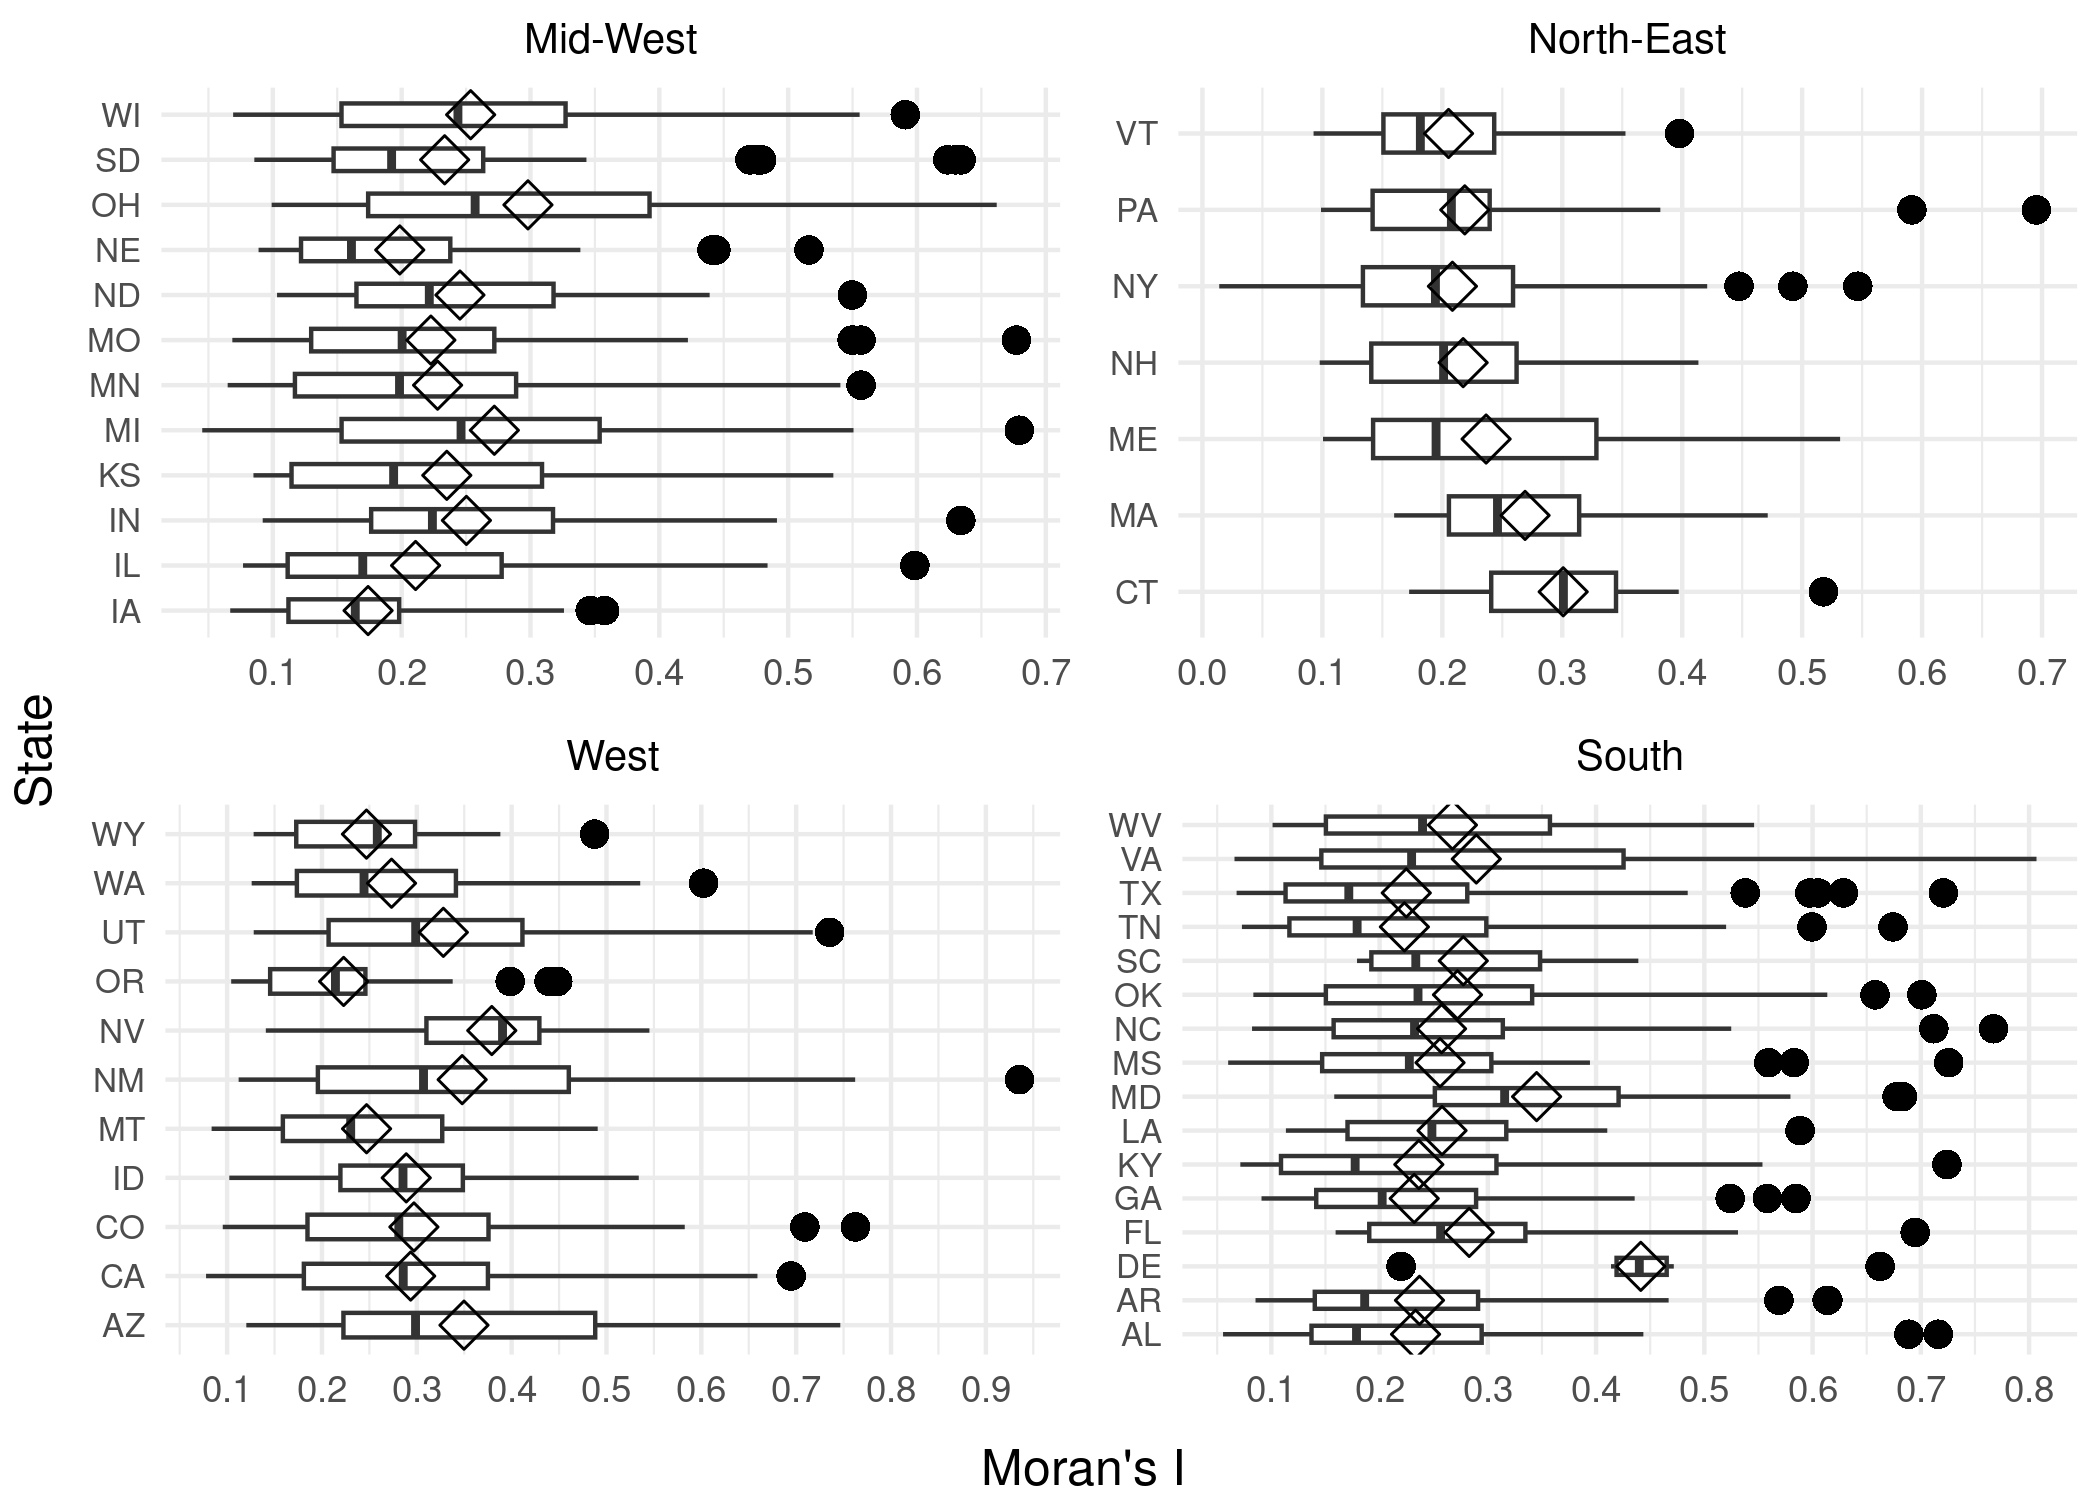
\includegraphics[width=1\textwidth, height=12cm]{plots/moran_state.png}
     \caption{Boxplot of Moran's I by Region}
     \label{fig:moran_region}
 \end{figure}

 \begin{figure}[htbp]
    \centering
     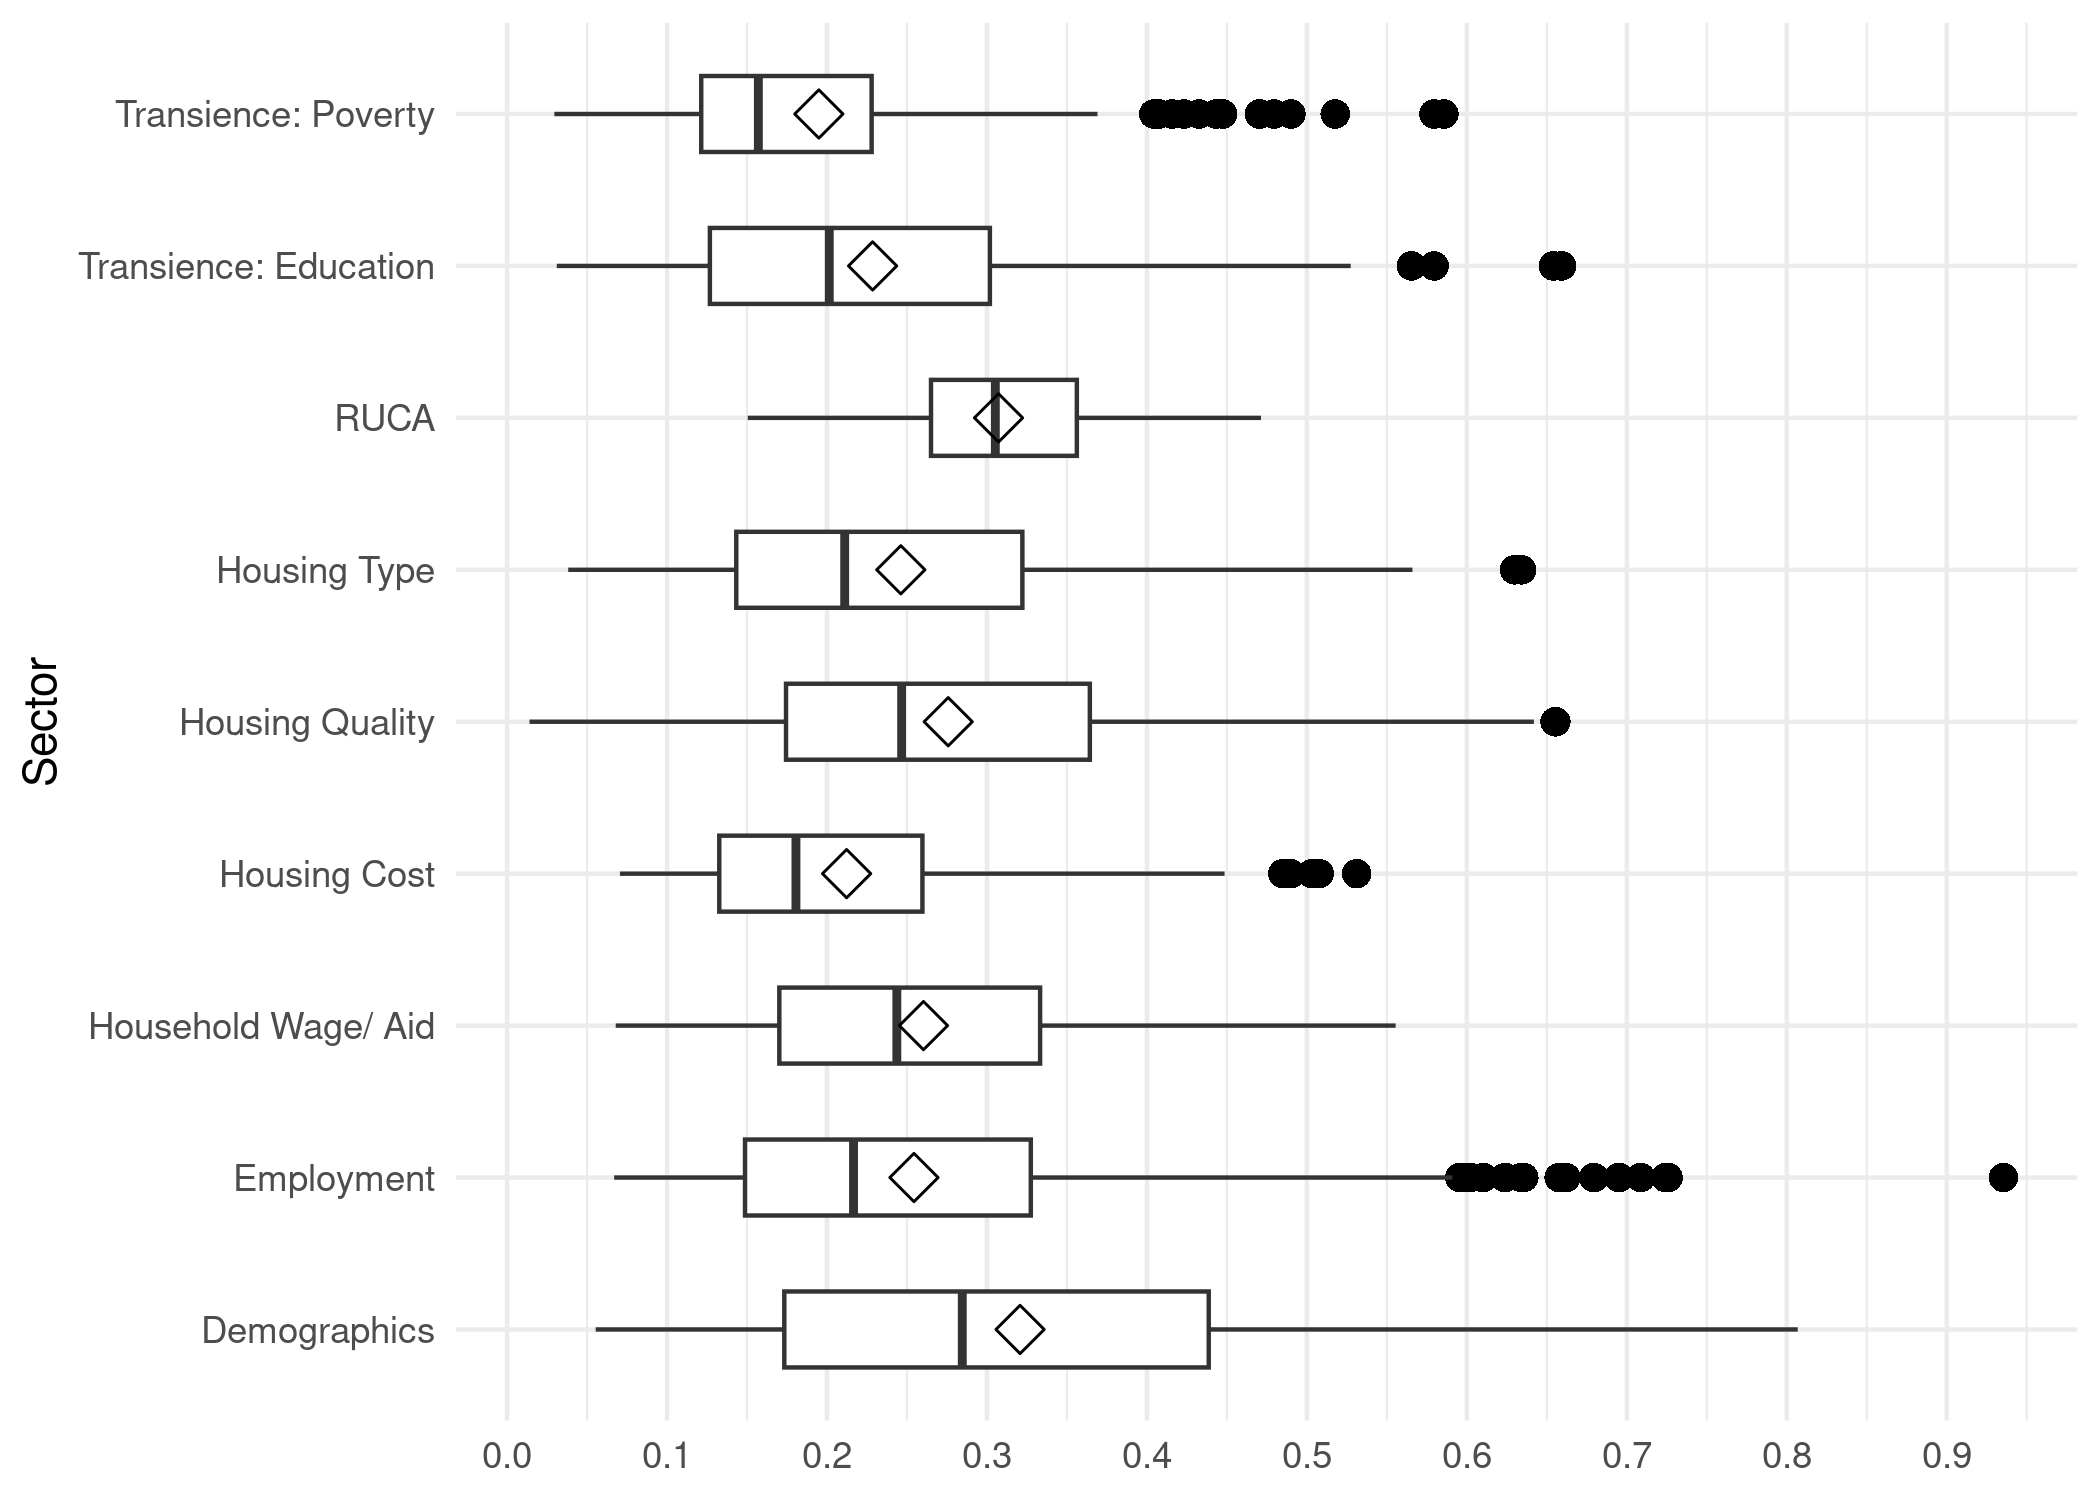
\includegraphics[width=1\textwidth, height=10cm]{plots/moran_sector}
     \caption{Boxplot of Moran's I by Sector}
     \label{fig:moran_sector}
 \end{figure}




\section{\textit{Multinomial Logistic Regression}}

The final method applied in this study is a multinomial logistic regression performed on each sector of data and tested on the data for each state. The probability that a predicted risk level is the actual risk level is used to measure how well the data for each state can be predicted based on a model trained on the other states alongside the confusion matrices for each sector's actual and predicted classification. National models using in-sample evaluation are used to measure how well a census tract's risk levels can be predicted.

\subsection{Probability}

\begin{figure}[htbp]
    \centering
     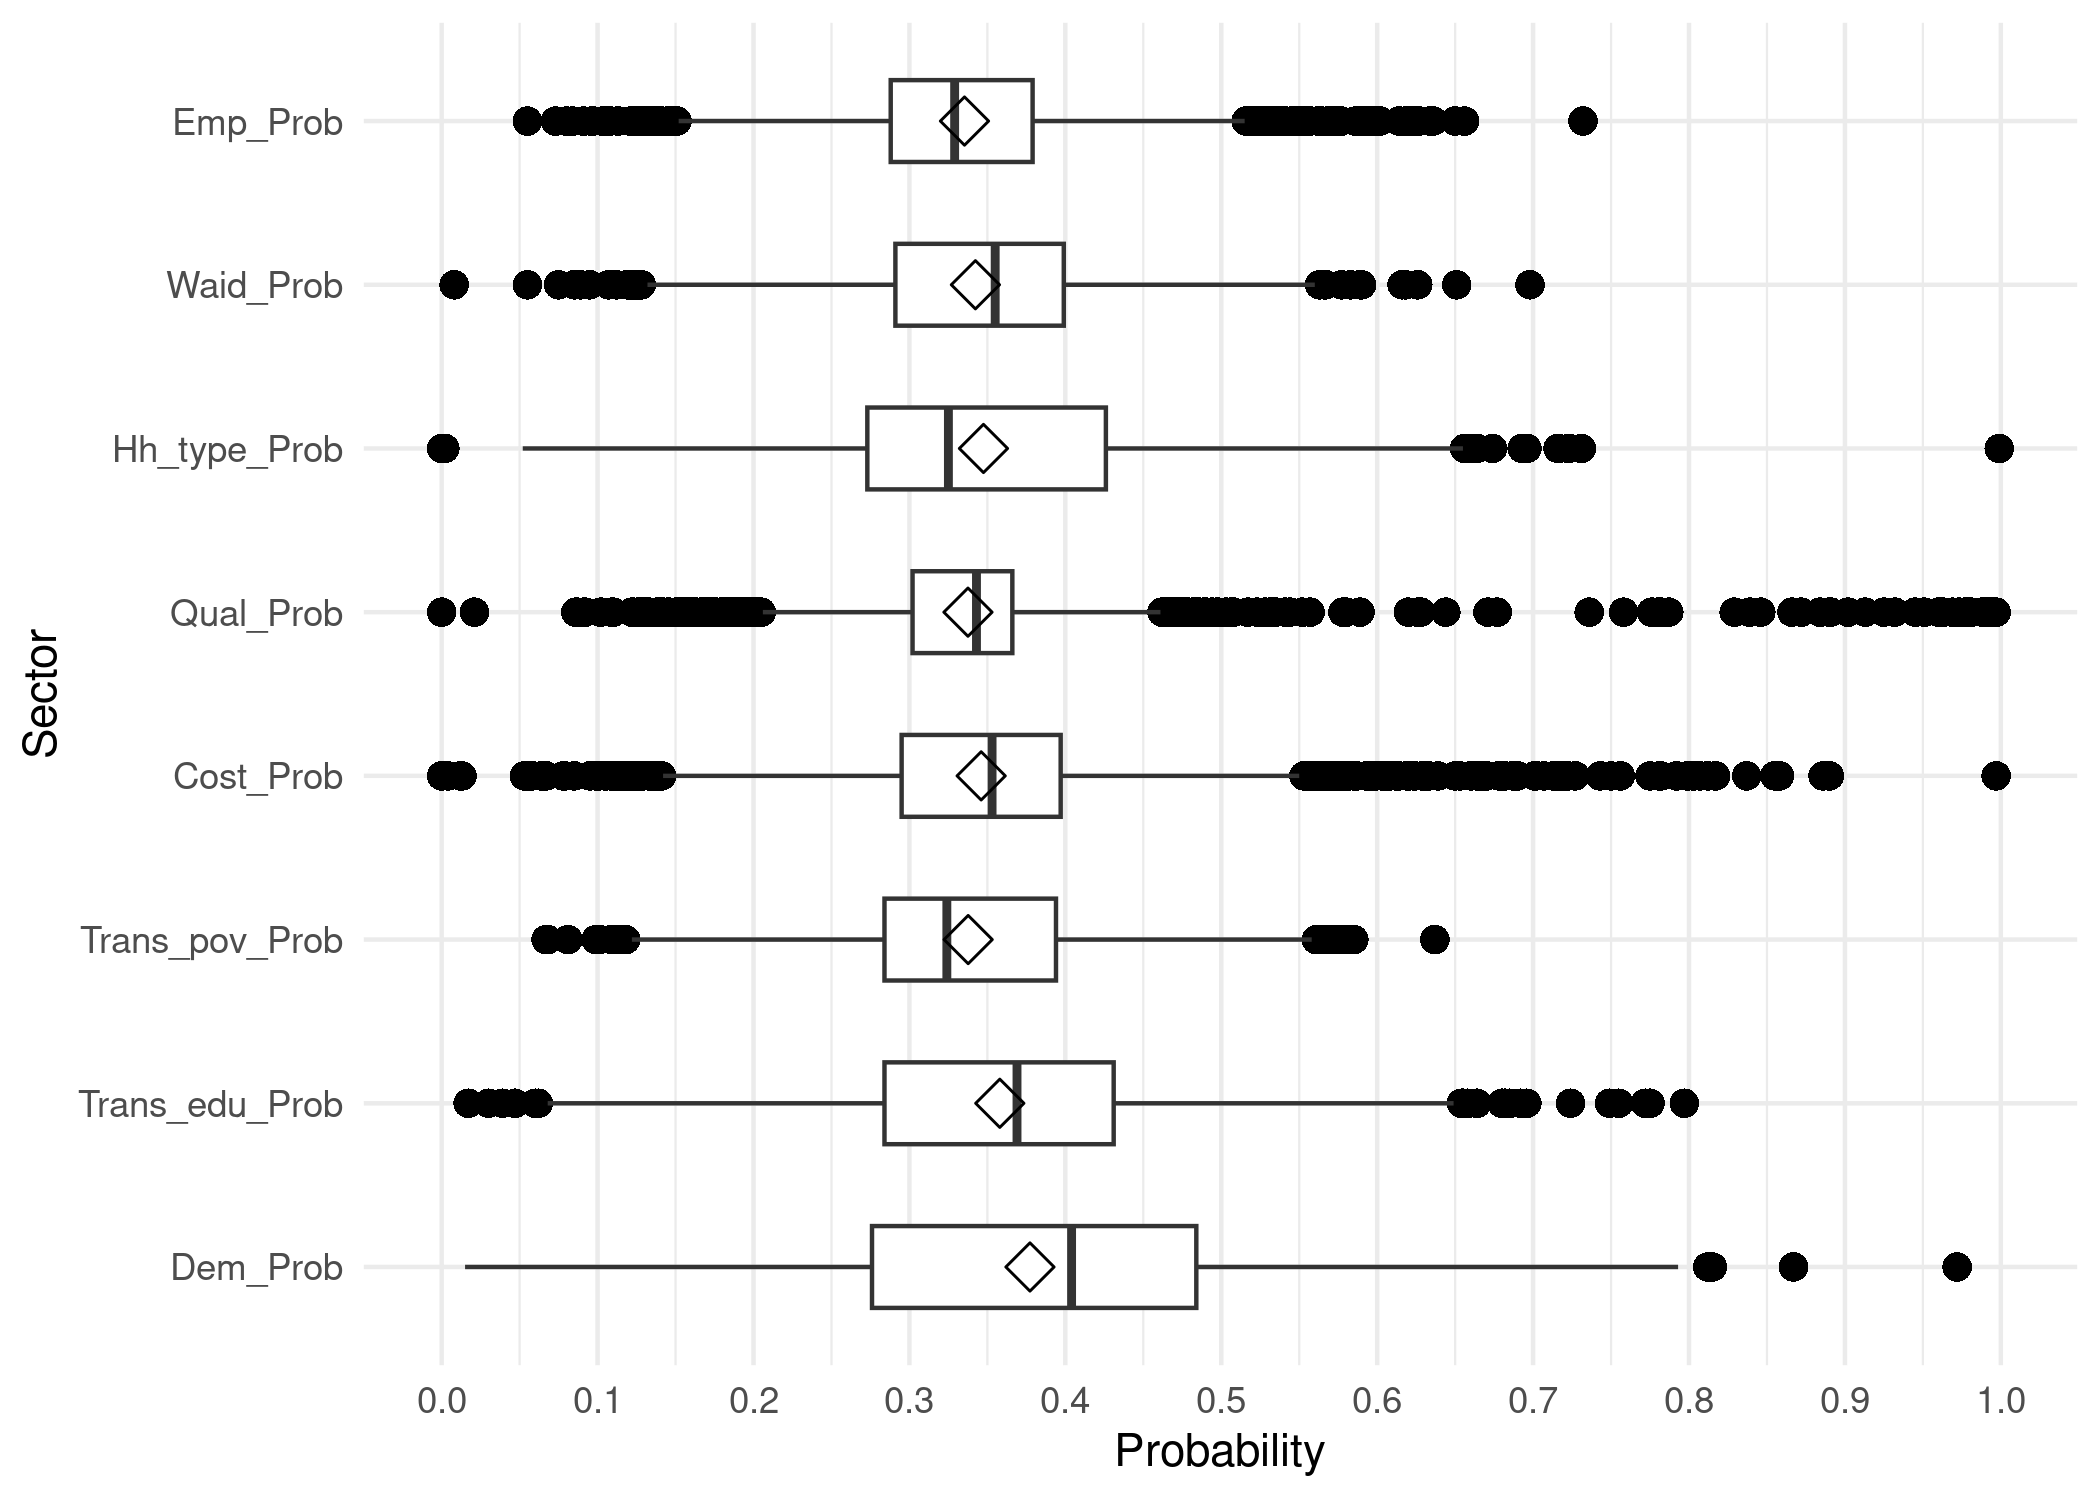
\includegraphics[width=1\textwidth, height=10cm]{plots/prob_sector.png}
     \caption{Boxplot of Moran's I by Sector}
     \label{fig:prob_sector}
 \end{figure}

The average probability for all sectors was low as demonstrated by Figure~\ref{fig:prob_sector}: employment diversity, housing quality, RMP and household factors had an average probability of 34 percent; housing type and housing cost had an average of 0.35; RMP had an average of 36 percent; demographics had the highest average probability at 0.38. Demographics also had the highest standard deviation at 14 percent, indicating a high degree of variation in predictability. For each sector in each state, Utah had the best prediction results with an average of 41 percent and Minnesota was the hardest to predict at 31 percent between sectors. Average probabilities for each cluster across sectors were similarly low. Across every sector except demographics, the models predicted the highest average probabilities for low-risk level census tracts. For demographics, the models had the highest average probability for the medium-risk level census tracts. Figure~\ref{fig:prob_sector} Shows the distribution of average probability for each state. With an average of 0.35, no states performed well across sectors. One last area of interest is any trends that may exist between the probabilities for each sector. Figure~\ref{fig:prob_corr} Shows that there are no significant correlations between the probabilities across sectors. The following subsections explore the performance of the state models and national models for each sector. 

\begin{figure}[htbp]
    \centering
     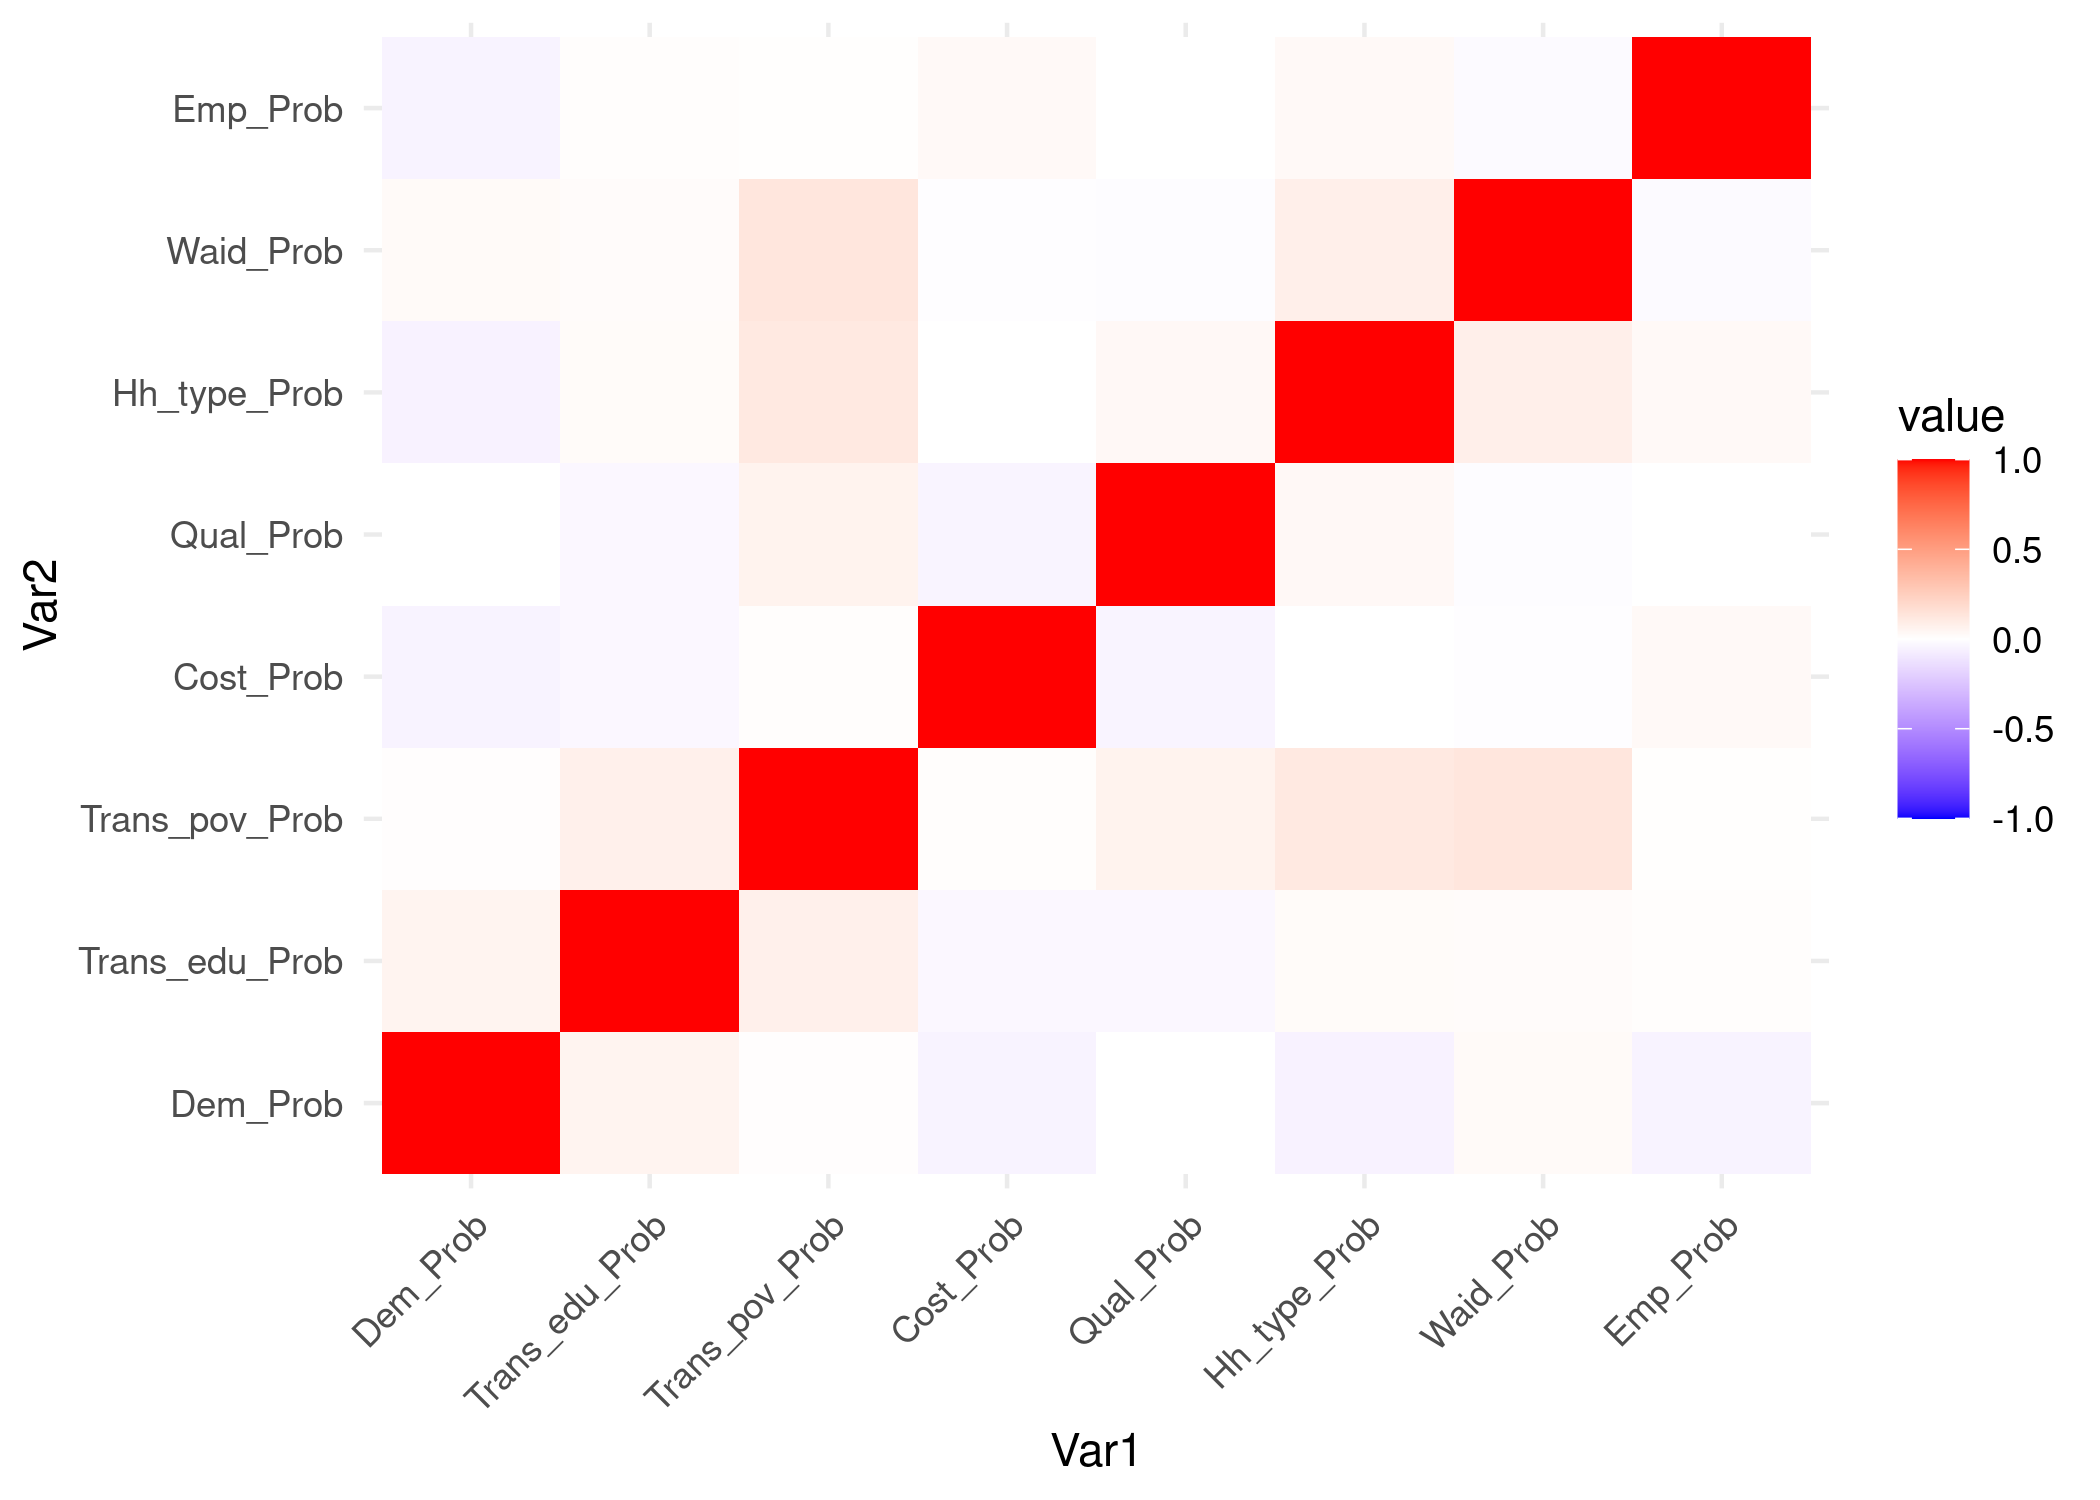
\includegraphics[width=1\textwidth, height=12cm]{plots/prob_corr.png}
     \caption{Correlation Plot of Sector Probabilities}
     \label{fig:prob_corr}
 \end{figure}

\begin{figure}[htbp]
    \centering
     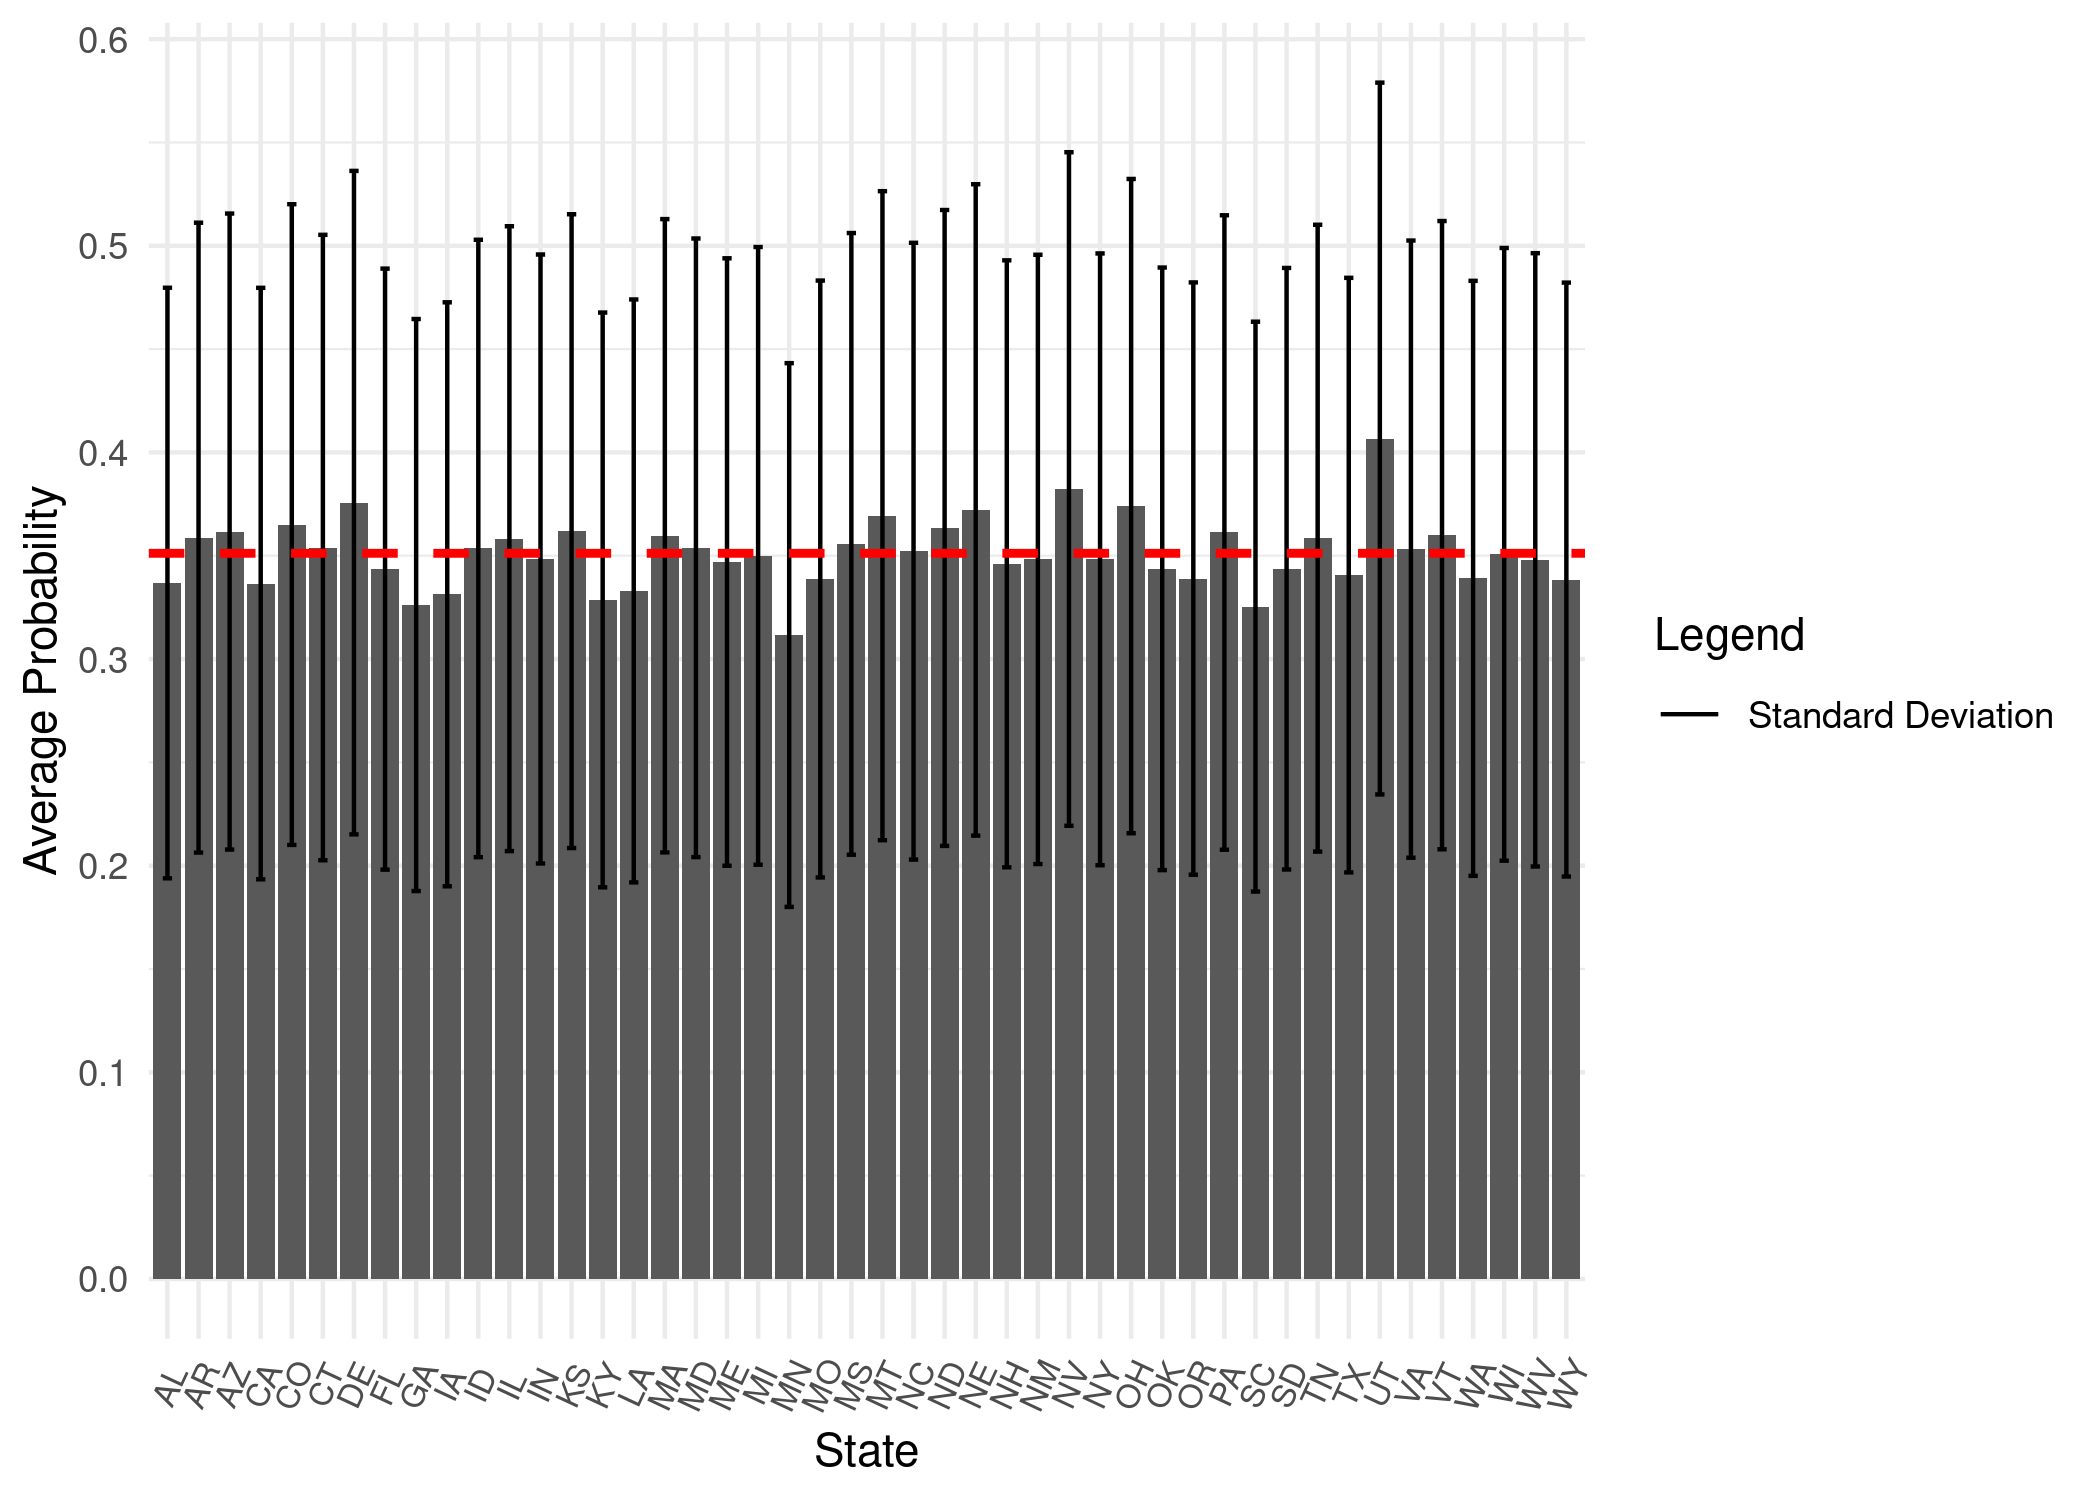
\includegraphics[width=1\textwidth, height=12cm]{plots/prob_state.png}
     \caption{Bar Graph of Average Probabilities by State with Error Bars}
     \label{fig:prob_sector}
 \end{figure}


\subsection{Accuracy}
The confusion matrices for each sector show that accuracy is low, with the models for most sectors over-classifying census tracts as low risk significantly harmed their accuracy. Presented here are also the accuracy results for national models tested using in-sample evaluation to measure accuracy under the best-case scenario. 

Table~\ref{tab:emp_confusion} shows that the models struggled to classify the medium-risk levels and high-risk levelss with the best performance on the low-risk levels for the economic diversity sector. These models were more successful at classifying census tracts with higher levels of economic diversity. The state models correctly classified 34 percent of low-risk census tracts, 11 percent of medium-risk census tracts, and 53 percent of low-risk census tracts. Overall, the state models were 34 percent accurate and the national model was 41 percent accurate. 

\begin{table}[!htbp]
    \small
    \centering
    \caption{Employment Confusion Matrix and Statistics}
    \label{tab:emp_confusion}
    \begin{tabular}{lccc}
        \toprule
        & \textbf{High Risk} & \textbf{Medium Risk} & \textbf{Low Risk} \\
        \midrule
        \textbf{High Risk} & 708 & 675 & 654 \\
        \textbf{Medium Risk} & 386 & 232 & 431 \\
        \textbf{Low Risk} & 987 & 1051 & 1238 \\
        \bottomrule
    \end{tabular}
\end{table} 


The demographic diversity models were able to predict medium-risk levels and low-risk levels significantly better than high-risk levels for the demographic diversity sector.  Table~\ref{tab:dem_confusion} shows The models were most capable of predicting medium-risk level census tracts. The models accurately predicted three percent of high-risk level census tracts while classifying medium-risk census tracts with 72 percent accuracy and 42 percent of low-risk census tracts. The state and national models predicted 48 and 52 percent of census tracts accurately. 

\begin{table}[!htbp]
    \small
    \centering
    \caption{Demographics Confusion Matrix and Statistics}
    \label{tab:dem_confusion}
    \begin{tabular}{lccc}
        \toprule
        & \textbf{High Risk} & \textbf{Medium Risk} & \textbf{Low Risk} \\
        \midrule
        \textbf{High Risk} & 48 & 95 & 76 \\
        \textbf{Medium Risk} & 843 & 1975 & 1274 \\
        \textbf{Low Risk} & 378 & 666 & 1007 \\
        \bottomrule

    \end{tabular}
\end{table} 

Table~\ref{tab:cost_confusion} shows that the housing cost models struggled to classify all census tracts. They also struggled to differentiate between medium-risk levels and high-risk-level census tracts. The state models accurately predicted 34 percent of high-risk level census tracts, 44 percent of medium-risk level census tracts, and 43 percent of low-risk level census tracts. The state models were 45 percent accurate and the national model was 41 percent accurate. 

\begin{table}[!htbp]
    \small
    \centering
    \caption{Housing Cost Confusion Matrix and Statistics}
    \label{tab:cost_confusion}
    \begin{tabular}{lccc}
        \toprule
        & \textbf{High Risk} & \textbf{Medium Risk} & \textbf{Low Risk} \\
        \midrule
        \textbf{High Risk} & 669 & 446 & 422 \\
        \textbf{Medium Risk} & 660 & 962 & 817 \\
        \textbf{Low Risk} & 625 & 803 & 938 \\
        \bottomrule
    \end{tabular}
\end{table} 

Table~\ref{tab:qual_confusion} shows that the housing quality models significantly over-classified census tracts as low-risk levels. The state models correctly classified 15 percent of high-risk census tracts, 13 percent of medium-risk level census tracts, and 63 percent of low-risk level census tracts. Overall, the state models had 39 percent accuracy and the national model had 32 percent accuracy. 

\begin{table}[!htbp]
    \small
    \centering
    \caption{Housing Quality Confusion Matrix and Statistics}
    \label{tab:qual_confusion}
    \begin{tabular}{lccc}
        \toprule
        & \textbf{High Risk} & \textbf{Medium Risk} & \textbf{Low Risk} \\
        \midrule
        \textbf{High Risk} & 285 & 278 & 179 \\
        \textbf{Medium Risk} & 592 & 296 & 673 \\
        \textbf{Low Risk} & 954 & 1632 & 1458 \\
        \bottomrule

    \end{tabular}
\end{table} 

Table~\ref{tab:trans_edu_confusion} shows that the  RME models significantly over-classified census tracts as low-risk levels. They successfully predicted 14 percent of low-risk census tracts, 39 percent of medium-risk level census tracts, and  60 percent of low-risk census tracts. The state models had an accuracy of 46 percent and the national model had an accuracy of 42 percent.

\begin{table}[!htbp]
    \small
    \centering
    \caption{Confusion Matrix and Statistics}
    \label{tab:confusion}
    \begin{tabular}{lccc}
        \toprule
        & \textbf{High Risk} & \textbf{Medium Risk} & \textbf{Low Risk} \\
        \midrule
        \textbf{High Risk} & 219 & 200 & 197 \\
        \textbf{Medium Risk} & 427 & 881 & 810 \\
        \textbf{Low Risk} & 917 & 1169 & 1542 \\
        \bottomrule
        \midrule
        Precision & 0.36 & 0.42 & 0.43 \\
        Recall & 0.14 & 0.39 & 0.6 \\
        F1 & 0.2 & 0.4 & 0.5 \\
        Prevalence & 0.25 & 0.35 & 0.4 \\
        Detection Rate & 0.03 & 0.14 & 0.24 \\
        Detection Prevalence & 0.1 & 0.33 & 0.57 \\
        Balanced Accuracy & 0.53 & 0.55 & 0.53 \\
        \bottomrule
    \end{tabular}
\end{table} 

Table~\ref{tab:trans_pov_confusion} shows that the RMP models significantly over-classified census tracts as low-risk levels. They successfully predicted 15 percent of high-risk census tracts, 14 percent of medium-risk census tracts, and 72 percent of high-risk census tracts. The state models had an accuracy of 41 percent and the national model had an accuracy of 37 percent. 

\begin{table}[!htbp]
    \small
    \centering
    \caption{Residential Mobility: Poverty Confusion Matrix and Statistics}
    \label{tab:trans_pov_confusion}
    \begin{tabular}{lccc}
        \toprule
        & \textbf{High Risk} & \textbf{Medium Risk} & \textbf{Low Risk} \\
        \midrule
        \textbf{High Risk} & 298 & 394 & 353 \\
        \textbf{Medium Risk} & 420 & 287 & 324 \\
        \textbf{Low Risk} & 1182 & 1356 & 1748 \\
        \bottomrule

    \end{tabular}
\end{table} 

Table~\ref{tab:waid_confusion} shows that the household factor models significantly over-classified census tracts as low-risk levels. They successfully predicted 12 percent of high-risk level census tracts, 33 percent of medium-risk level census tracts, and 54 percent of low-risk level census tracts. The state models had an accuracy of 42 percent and the national model had an accuracy of 36 percent. 

\begin{table}[!htbp]
    \small
    \centering
    \caption{Household Factors Confusion Matrix and Statistics}
    \label{tab:waid_confusion}
    \begin{tabular}{lccc}
        \toprule
        & \textbf{High Risk} & \textbf{Medium Risk} & \textbf{Low Risk} \\
        \midrule
        \textbf{High Risk} & 195 & 163 & 208 \\
        \textbf{Medium Risk} & 492 & 748 & 897 \\
        \textbf{Low Risk} & 972 & 1352 & 1335 \\
        \bottomrule
    \end{tabular}
\end{table}

Table~\ref{tab:hh_type_confusion} shows that the housing type models significantly over-classified census tracts as low-risk levels. they successfully predicted 6 percent of low-risk level census tracts, 33 percent of medium-risk level census tracts, and 54 percent of high-risk census tracts. The state models had an accuracy of 45 percent and the national models had an accuracy of 43 percent. 

\begin{table}[!htbp]
    \small
    \centering
    \caption{Housing Type Confusion Matrix and Statistics}
    \label{tab:hh_type_confusion}
    \begin{tabular}{lccc}
        \toprule
        & \textbf{High Risk} & \textbf{Medium Risk} & \textbf{Low Risk} \\
        \midrule
        \textbf{High Risk} & 195 & 163 & 208 \\
        \textbf{Medium Risk} & 492 & 748 & 897 \\
        \textbf{Low Risk} & 972 & 1352 & 1335 \\
        \bottomrule

    \end{tabular}
\end{table}

\section{\textit{Rurality and Risk Levels}}

The following table shows the local spatial autocorrelation for each cluster across each sector. There are notable local Moran's I statistics for low and high-risk level census tracts. The medium-risk level census tracts had negligible local Moran's I statistics. The results indicate that the extremes of the scale tend to cluster around each other: high-risk census tracts are close to high-risk census tracts and low-risk census tracts are close to low-risk census tracts while there is a level of spatial randomness in the grouping of medium-risk level census tracts. 

\begin{table}[ht]
    \centering
    \caption{Local Morans I Risk-Level Results}
    \label{tab:local_moran}
    \begin{tabular}{lrrr}
      \hline
    sector & c1 & c2 & c3 \\ 
      \hline
    emp\_cluster & 0.83 & 0.00 & 0.89 \\ 
    \hline
      dem\_cluster & 2.09 & 0.14 & 0.58 \\ 
      \hline
      trans\_edu\_cluster & 1.28 & 0.10 & 0.25 \\ 
      \hline
      trans\_pov\_cluster & 1.16 & 0.05 & 0.48 \\ 
      \hline
      cost\_cluster & 0.79 & -0.00 & 0.57 \\ 
      \hline
      qual\_cluster & 1.06 & 0.00 & 0.74 \\ 
      \hline
      hhtype\_cluster & 0.91 & -0.00 & 0.68 \\ 
      \hline
      waid\_cluster & 1.52 & 0.09 & 0.22 \\ 
       \hline
    \end{tabular}
    \end{table}

To better understand housing insecurity risk in rural areas, it is important to look at the risk levels as they relate to the scale of rurality. Table~\ref{tab:ruca_risk} shows the percentage of each RUCA code that has a high-risk level for each sector. While RUCA code 10 makes up 50 percent of all census tracts, 43 to 50 percent of all high-risk level census tracts have this RUCA code. RUCA code 7 is next with a range between 32 and 39 percent of high-risk level census tracts while making up only 33 percent of the dataset. At the opposite end of the spectrum, RUCA code 9 makes up 5 percent of the dataset and only 5 percent of high-risk census tracts. Figure~\ref{fig:regional_map} shows the risk level of each census tract across each sector. Each census tract is assigned a color red (high-risk), yellow (medium-risk), and green (low-risk) for each sector. These colors are then saturated based on the probability for each sector. The colors are then blended so that the map reflects how well the state fits into its national train-split model and the overall risk level of the census tract. Many census tracts fall somewhere between green and yellow, with pockets of light shades of red visible. 

\begin{table}[ht]
    \caption{High-Risk Census Tract RUCA Breakdown}
    \label{tab:ruca_risk}
    \small
    \centering
    \begin{tabular}{rlll}
        \hline
       & sector & RUCA & Pct \\ 
        \hline
      1 & Qual\_Cluster & 10 & 0.5 \\ 
        2 & Emp\_Cluster & 10 & 0.49 \\ 
        3 & Dem\_Cluster & 10 & 0.49 \\ 
        4 & Cost\_Cluster & 10 & 0.49 \\ 
        5 & Waid\_Cluster & 10 & 0.49 \\ 
        6 & Trans\_POV\_Cluster & 10 & 0.48 \\ 
        7 & Trans\_EDU\_Cluster & 10 & 0.46 \\ 
        8 & Hhtype\_Cluster & 10 & 0.43 \\ 
        9 & Trans\_EDU\_Cluster & 7 & 0.39 \\ 
        10 & Hhtype\_Cluster & 7 & 0.37 \\ 
        11 & Waid\_Cluster & 7 & 0.35 \\ 
        12 & Emp\_Cluster & 7 & 0.34 \\ 
        13 & Trans\_POV\_Cluster & 7 & 0.34 \\ 
        14 & Cost\_Cluster & 7 & 0.33 \\ 
        15 & Qual\_Cluster & 7 & 0.33 \\ 
        16 & Dem\_Cluster & 7 & 0.32 \\ 
        17 & Hhtype\_Cluster & 8 & 0.15 \\ 
        18 & Dem\_Cluster & 8 & 0.14 \\ 
        19 & Trans\_POV\_Cluster & 8 & 0.13 \\ 
        20 & Cost\_Cluster & 8 & 0.13 \\ 
        21 & Qual\_Cluster & 8 & 0.13 \\ 
        22 & Emp\_Cluster & 8 & 0.12 \\ 
        23 & Waid\_Cluster & 8 & 0.11 \\ 
        24 & Trans\_EDU\_Cluster & 8 & 0.1 \\ 
        25 & Emp\_Cluster & 9 & 0.05 \\ 
        26 & Dem\_Cluster & 9 & 0.05 \\ 
        27 & Trans\_POV\_Cluster & 9 & 0.05 \\ 
        28 & Cost\_Cluster & 9 & 0.05 \\ 
        29 & Qual\_Cluster & 9 & 0.05 \\ 
        30 & Hhtype\_Cluster & 9 & 0.05 \\ 
        31 & Trans\_EDU\_Cluster & 9 & 0.04 \\ 
        32 & Waid\_Cluster & 9 & 0.04 \\ 
         \hline
      \end{tabular}
      \end{table}

\begin{figure}[htbp]
    \centering
     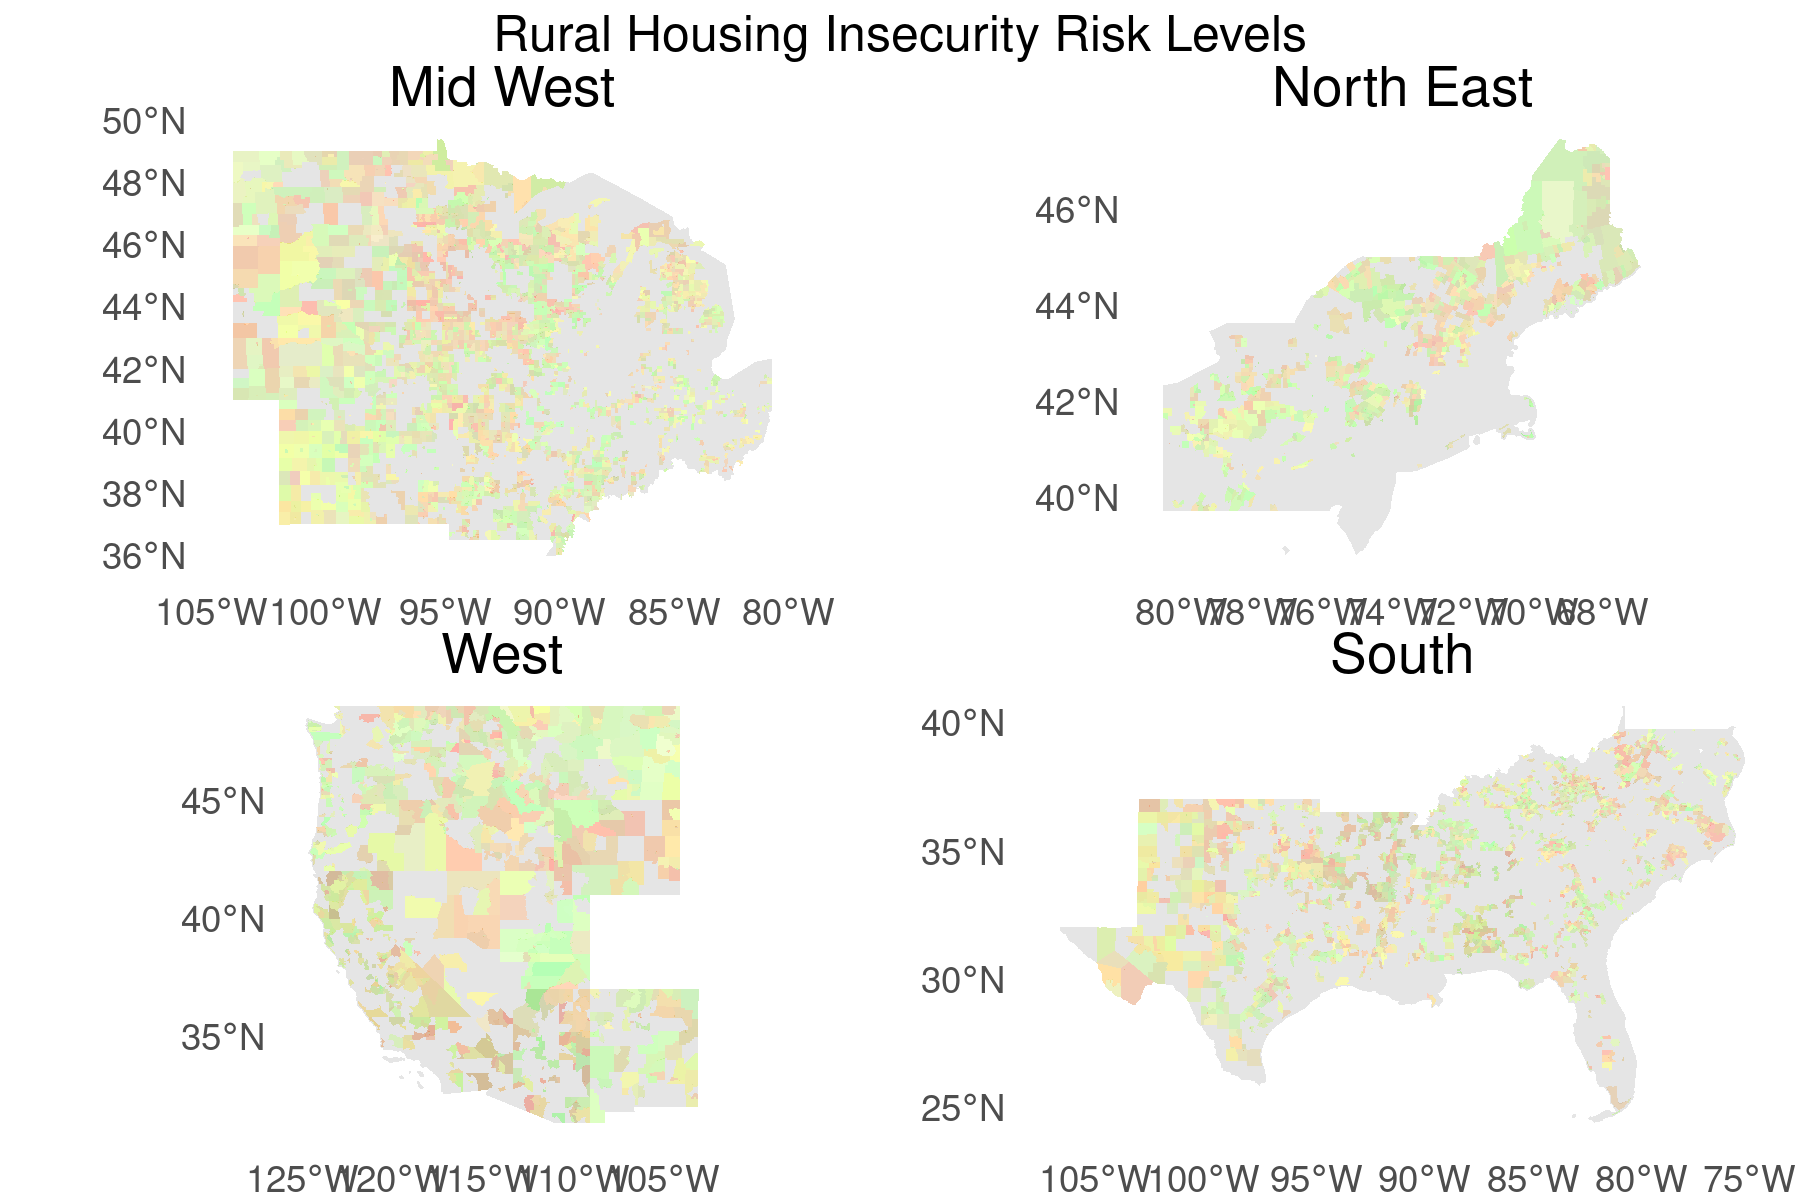
\includegraphics[width=\textwidth, height=12cm]{plots/regional_map.png}
     \caption{Risk Level Across Sectors}
     \label{fig:regional_map}
 \end{figure}


 
 The census tract risk threshold results in 115 census tracts labeled as high risk and 661 labeled as medium risk based on the sum of their risk level variables. Figure~\ref{fig:regional_risk_map} highlights the high-risk areas in red, and the medium-risk levels in yellow. The majority of the high-risk census tracts are in Minnesota (26), Wisconsin (26), Texas (24), Arizona (21), Missouri (18), Georgia (16), North Carolina (13), Montana (11), North Dakota (11), and Oklahoma (10). The other 104 high-risk census tracts are spread across 27 other states. % more on medium-risk census tracts

 \begin{figure}[htbp]
    \centering
     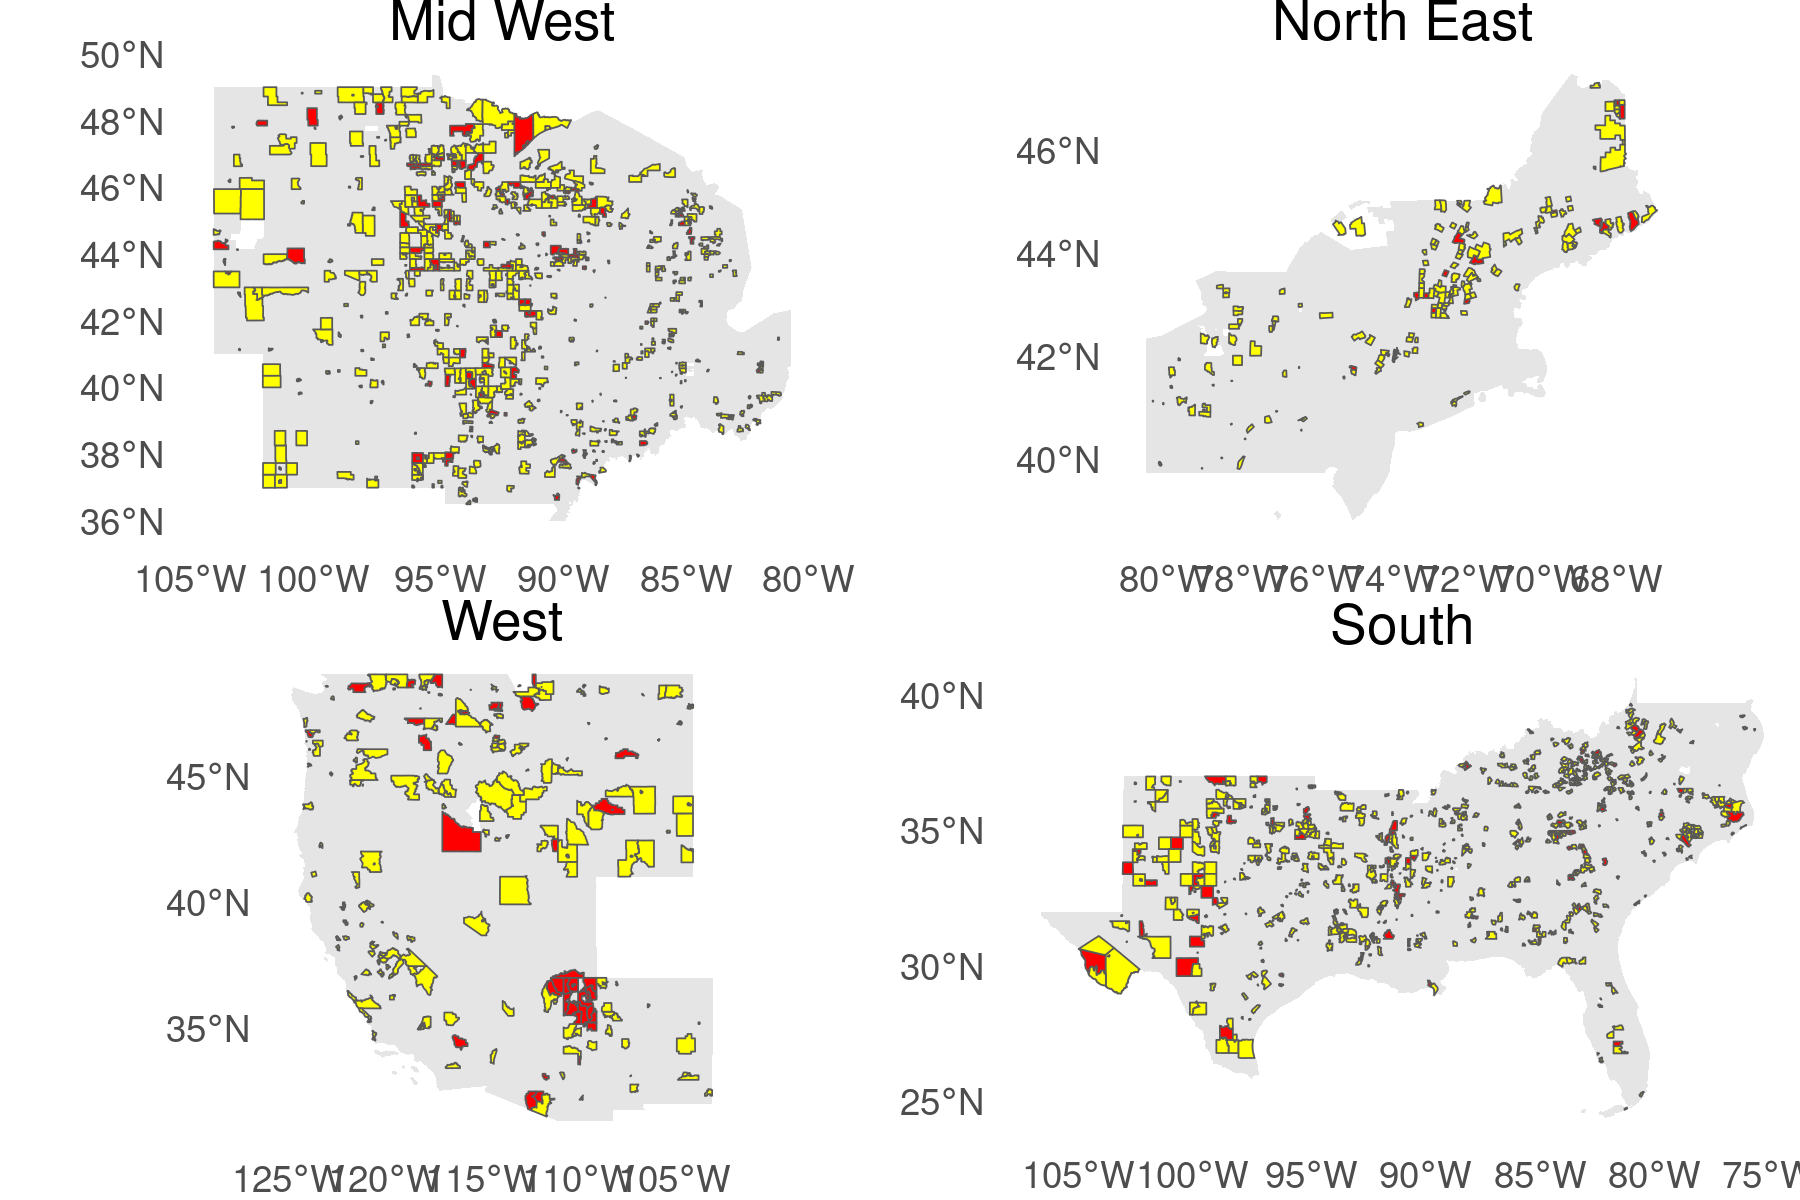
\includegraphics[width=\textwidth, height=12cm]{plots/regional_risk_map.png}
     \caption{Risk Level Across Sectors}
     \label{fig:regional_risk_map}
 \end{figure}

There are several important observations to be made from the high, medium, and low-risk census tracts. First, high and medium-risk census tracts have higher African-American and Hispanic/Latino populations as well as smaller white populations.  There are more people with a high school diploma and fewer people below the poverty line in low-risk census tracts. High and medium-risk census tracts have similar levels of high-cost mortgage and high-cost renter households but different levels of high-cost households without a mortgage. There is slightly greater usage of public assistance and supplemental security index usage in high and medium-risk census tracts. It should be noted that the standard t-test found no statistically significant differences between variable averages of the high-risk and low-risk census tracts and the medium-risk and low-risk census tracts. It should be noted that the averages do not account well for the variation in rural areas, so this can only be interpreted to indicate a lack of a national difference between risk levels of census tracts. 

\endinput
\chapter{Discussion}	

\hl{How can risk factors of be used to identify risk levels of housing insecurity while accounting for the variation in rural areas?}

The analysis of this thesis used the 4 C's of housing insecurity theoretical framework with American Community Survey data to identify risk levels of housing insecurity in a way that accounts for the variation in rural communities. The cluster analysis highlights the variation that exists in rural areas.

\hl{Do housing insecurity factors identified for urban areas exhibit similar characteristics in rural areas?}

\hl{When measuring housing insecurity across different dimensions, how often do the same features arise?}

\hl{Are there spatial relations between the different dimensions of housing insecurity?}

\hl{To what extent can the housing insecurity dimensions be predicted?}



\section{\textit{Employment Diversity}}

There are \hl{?} observations to be made from the employment diversity cluster analysis. First, at over 9 percent, the data shows that employment in education, health, and social work contributes significantly to employment in rural areas. The cluster medians for all three clusters are almost double the next highest values in retail trade and manufacturing. Next, wholesale trade and information employment make up relatively small parts of the rural economy with less than 1 percent across all cluster medians. The cluster medians for the catch-all "rural jobs" variable, incorporating agriculture, forestry, fishing, hunting, and mining, falls in the middle in terms of contributing to rural economies. This highlights the shift from agricultural to manufacturing that rural economies have made over the last several decades (\hl{source}). 

\section{\textit{Demographics}}
There are \hl{?} observations to be made from the demographic diversity cluster analysis. First, the data indicate that rural areas are predominantly white, with cluster medians ranging from 92 to 94 percent white. However, as previous research has indicated (\hl{source}), there are pockets of large minority populations and this is captured by the cluster analysis as demonstrated by the cluster with the lowest white population having the highest African American, Hispanic and Latino, and Other populations. The age and gender variables reflect a similar distribution of men and women over and under 18. As found by (\hl{source}), the data indicate that rural areas have a much larger older population than younger population with cluster medians falling between 9 and 11 percent for both under-18 variables. 


\section{\textit{Housing Cost}}
The cluster medians of the housing cost sector indicate that rural areas show a similar trend in housing costs. The cluster medians for the high-cost renters variable are almost three times as high as the next highest cluster medians, for the mortgage high-cost variable. One important factor in rural areas that has not been taken into account for housing costs is the widespread presence of official or unofficial mobile home parks. The effects of these structures on rural housing costs require further research to be fully understood. Another notable observation is that the cluster with the most high-cost renters also has the most high-cost homeowners without a mortgage. This indicates there may be some clustering of the different categories of housing cost.


\section{\textit{Housing Quality}}

The cluster medians of the housing quality section indicate that the ratio of occupied to unoccupied housing with incomplete plumbing or kitchen facilities is significant. The cluster medians for the incomplete facilities variables range from 17 to 25 percent while the medians for the occupied housing variables are never greater than 0.64 percent. This sector is severely limited because these were the only ACS variables that capture housing conditions. More factors are needed to fully encapsulate housing conditions, but these variables can at least highlight areas that show signs of poor housing conditions. 


\section{\textit{Residential Mobility: Education}}
Rates of residential mobility for the education sector were low, the highest cluster median is the variable for those who moved in the same county with a high school degree at 1.36 percent. The cluster medians for the same house with a high school degree variable ranges from 22 to 23 percent, making the category with the most stable situation far greater than those who moved even when all transiency variables are combined. One note of concern is in all three clusters, 7 percent of the population did not move, but do not have a high school diploma. While stable for the year for which they were interviewed, their education status puts them at risk for housing instability. 

\section{\textit{Residential Mobility: Poverty}}
There are \hl{?} observations to be made from the residential mobility: poverty cluster analysis. First, the cluster medians for same house below the poverty line are higher than the same house at 125 percent of the poverty level variable. This aligns with the rural pockets of poverty indicated by (\hl{source}). Next, Across cluster medians, the percent of the population in poverty or just above the poverty line is never greater than 1 percent. Finally, For transiency variables in this sector, moved in county below the poverty level has the highest cluster medians across all variables indicating that this group is the most present in the dataset. 

\section{\textit{Household Factors}}
There are \hl{?} observations to be made from the household factors cluster analysis. First, there is a significant conversation about income inequality in urban areas, yet the cluster medians for the Gini index are less than 0.5 indicating a low level of income inequality in rural areas. Next,  for each cluster median, at least a third of the population has no investment income or no other income, indicating that residents of rural areas are highly dependent on wages. The cluster medians for the number of households receiving public assistance range from four to five percent, indicating there may be a significant number of households eligible for public assistance that do not have it. The cluster medians for the number of households with more than three workers are less than two percent, indicating that this high-risk factor occupies a minority of households. 


\section{\textit{Housing Type}}

There are \hl{?} observations to be made from the housing type cluster analysis. First, single-unit homeowners are the primary means of housing in rural areas, with cluster medians ranging between 88 and 90 percent. The next most prominent type of housing is single-unit renters, with cluster medians ranging from 55 to 68 percent. This is significant given the previously mentioned levels of high-cost renters in rural areas. Numerous studies (\hl{insert sources}) have identified the harms of high-cost renting, but the extent to which these effects are the same in rural areas has not been identified. 


\section{\textit{Association Rules}}

The association rules show that the risk levels of each sector do not have a lot of common overlap. Of the four types of associations analyzed, there were no associations that occur more than expected by random chance. This means that rural areas, when space is not accounted for, have little commonality in terms of housing insecurity risk across the different sectors. This is unexpected under the 4 C's of housing insecurity framework where areas theoretically show similar signs across pillars. While the association rules did not find strong trends between risk levels, it does highlight pockets of rural census tracts where this commonality exists. These areas may be of interest to policy-makers and researchers for their communities. 

\section{\textit{Moran's I}}

When spatial relationships are accounted for, the results are very similar to the association rules. Of the 2,018 statistically significant Moran's I values, the average of 0.26 indicates that there are generally low spatial autocorrelations between variables from a wide lens. The sector averages tell a very similar story, ranging between 0.2 and 0.32 for each sector. These results indicate that rural areas do not have the same level of clustering as noted with many of the housing insecurity factors. The outliers highlighted in Chapter 4 point to areas of concern that further research should investigate. While the global Moran's I values do not indicate very high levels of spatial autocorrelation among factors, the local Moran's I analysis reveals that there are strong local spatial autocorrelations between high-risk and low-risk level census tracts across each sector. While these numbers are influenced by the way that census tracts were only clustered with relatively close census tracts, it provides some evidence for the clustering of housing insecurity risk levels in rural areas. Most notable is the level of spatial randomness for the medium-risk levels across sectors. The results indicate that the extreme clusters are spatially clustered but not in the middle area. 


\section{\textit{Multinomial Logistic Regression}}

The multinomial logistic regression results show that it is very difficult to predict the housing insecurity risk levels of census tracts based on other states and nationally. This provides evidence to one of the themes of rural research which emphasizes that rural areas vary greatly. The models also faced significant issues with over-classifying census tracts as low-risk. This could indicate that there is less variability in these census tracts, but this is not beneficial in terms of understanding rural housing insecurity. 

\section{Evaluating the 4 C's}

While this exploratory analysis has provided novel insights into rural housing insecurity and how the current scope of housing insecurity research can be adapted to rural areas, the results did not closely follow what is expected under the 4 C's of housing insecurity framework. There are three plausible explanations for this difference between the theoretical model and the results. First, the methodology used in this thesis does not adequately encapsulate the 4 C's of housing insecurity. Second, the urban lens of housing insecurity does not apply to rural areas enough for the same effects from the housing insecurity factors. Third, the 4 C's model of housing insecurity, potentially biased by the urban lens of housing insecurity, does not conform well to rural areas. 

\section{\textit{Previous Research}}

Due to the urban-centric lens towards housing insecurity, there is little previous research to compare this study to. Gleason et al. 2021 applied similar spatial techniques to census tracts in Maine found that poverty, unemployment, and high housing costs are common in rural and urban areas of Maine but found these results to be inaccurate in a later study (Gleason et al 2022?). Lichter and Johnson 2007 did a nationwide county-level analysis on poverty levels specific to rural areas. Insert authors that did research specific to rural areas. This is the first study of this scale to employ data mining techniques on rural housing insecurity. Also, it develops a methodology used with the 4 Cs of housing insecurity that can be applied to rural and urban areas while moving the focus further away from homelessness as a binary. 


\section{\textit{Limitations}}
As the American Community Survey samples less in rural areas, the accuracy of the data is limited in how accurately it represents the real-world. While the estimates are “likely reasonable approximations of the populations they represent”, small area estimates like census tracts used here have issues with attribute uncertainty (Spielman 2014, p#). Despite this, it is currently the most detailed source of data available for rural areas. The largest issue that needs to be addressed in rural housing insecurity research is the lack of factors uniquely identified to rural areas. This study relied on rural-specific literature as much as possible, but many of the works cited are from an urban lens. Future research should use this study as a starting point for giving housing insecurity and homelessness adequate attention. The most important direction is to identify community level risk factors unique to rural areas. Further studies should also use a wider range of data sources to capture sectors with few available variables such as housing conditions. From our spatial analysis there are several observations worthy of further investigation  
\chapter{Conclusion}	%Chapter title

Housing insecurity is difficult in several different ways. First, it is difficult to define. Until there is a full understanding of housing insecurity, which includes amending the gap between urban and rural housing insecurity research, we are limited in our ability to properly operationalize the meaning of the phrase. Second, it is difficult to study. As a concept that spans such a wide range of individual, social, and political factors is inherently difficult to study. Third, and most importantly, housing insecurity is difficult for those who experience it. In rural areas, these difficulties are compounded due to the urban-centric lens of housing insecurity that has developed over decades of primarily urban-oriented research. This initial exploration hopes to serve as a starting point for policy-makers and researchers to begin deconstructing the urban-centric lens and give those in rural populations the attention and resources they need and deserve. 

\endinput


\newpage % Start on a new page (optional)
%\section*{\bibname} % Section header for the bibliography (change to \refname or \references if needed)
\phantomsection
\addcontentsline{toc}{chapter}{\texorpdfstring{\MakeUppercase{\bibname}}{\bibname}}




\doublespacing % Adjust spacing as needed (e.g., \doublespacing, \onehalfspacing)
\bibliographystyle{plainnat} % Set the bibliography style to plainnat
\bibliography{references} % Specifies the BibTeX file		% Inserts and formats the reference section.

\appendix					% Include this before any appendices.
\chapter{Descriptive Statistics}	%Appendix title
\begin{table}[!htbp] \centering 
    \caption{Demographics Descriptive Statistics} 
    \label{} 
  \begin{tabular}{@{\extracolsep{5pt}}lD{.}{.}{-3} D{.}{.}{-3} D{.}{.}{-3} D{.}{.}{-3} D{.}{.}{-3} } 
  \\[-1.8ex]\hline 
  \hline \\[-1.8ex] 
  Statistic & \multicolumn{1}{c}{N} & \multicolumn{1}{c}{Mean} & \multicolumn{1}{c}{St. Dev.} & \multicolumn{1}{c}{Min} & \multicolumn{1}{c}{Max} \\ 
  \hline \\[-1.8ex] 
  white & 6,362 & 0.859 & 0.189 & 0.000 & 1.000 \\ 
  black & 6,362 & 0.067 & 0.150 & 0.000 & 1.000 \\ 
  am\_in\_ala\_nat & 6,362 & 0.028 & 0.115 & 0.000 & 0.992 \\ 
  asian & 6,362 & 0.006 & 0.012 & 0.000 & 0.283 \\ 
  haw\_pac & 6,362 & 0.001 & 0.003 & 0.000 & 0.133 \\ 
  other & 6,362 & 0.017 & 0.043 & 0.000 & 0.575 \\ 
  hisp\_lat & 6,362 & 0.076 & 0.133 & 0.000 & 0.995 \\ 
  male\_u18 & 6,362 & 0.110 & 0.032 & 0.000 & 0.276 \\ 
  female\_u18 & 6,362 & 0.105 & 0.031 & 0.000 & 0.396 \\ 
  male\_o18 & 6,362 & 0.391 & 0.055 & 0.000 & 1.000 \\ 
  female\_o18 & 6,362 & 0.394 & 0.045 & 0.000 & 1.000 \\ 
  \hline \\[-1.8ex] 
  \end{tabular} 
  \end{table} 


  \begin{table}[!htbp] \centering 
    \caption{RME Descriptive Statistics} 
    \label{} 
  \begin{tabular}{@{\extracolsep{5pt}}lD{.}{.}{-3} D{.}{.}{-3} D{.}{.}{-3} D{.}{.}{-3} D{.}{.}{-3} } 
  \\[-1.8ex]\hline 
  \hline \\[-1.8ex] 
  Statistic & \multicolumn{1}{c}{N} & \multicolumn{1}{c}{Mean} & \multicolumn{1}{c}{St. Dev.} & \multicolumn{1}{c}{Min} & \multicolumn{1}{c}{Max} \\ 
  \hline \\[-1.8ex] 
  same\_house\_less\_than\_hs & 6,362 & 0.084 & 0.048 & 0.000 & 0.495 \\ 
  same\_house\_hs & 6,362 & 0.231 & 0.060 & 0.000 & 0.667 \\ 
  moved\_in\_county\_less\_than\_hs & 6,362 & 0.005 & 0.007 & 0.000 & 0.079 \\ 
  moved\_in\_county\_hs & 6,362 & 0.012 & 0.010 & 0.000 & 0.083 \\ 
  moved\_diff\_county\_less\_than\_hs & 6,362 & 0.004 & 0.008 & 0.000 & 0.134 \\ 
  moved\_diff\_county\_hs & 6,362 & 0.008 & 0.011 & 0.000 & 0.169 \\ 
  moved\_diff\_state\_less\_than\_hs & 6,362 & 0.001 & 0.003 & 0.000 & 0.090 \\ 
  moved\_diff\_state\_hs & 6,362 & 0.003 & 0.005 & 0.000 & 0.080 \\ 
  \hline \\[-1.8ex] 
  \end{tabular} 
  \end{table} 

\begin{table}[!htbp] \centering 
\caption{RMP Descriptive Statistics} 
\label{} 
\begin{tabular}{@{\extracolsep{5pt}}lD{.}{.}{-3} D{.}{.}{-3} D{.}{.}{-3} D{.}{.}{-3} D{.}{.}{-3} } 
\\[-1.8ex]\hline 
\hline \\[-1.8ex] 
Statistic & \multicolumn{1}{c}{N} & \multicolumn{1}{c}{Mean} & \multicolumn{1}{c}{St. Dev.} & \multicolumn{1}{c}{Min} & \multicolumn{1}{c}{Max} \\ 
\hline \\[-1.8ex] 
same\_house\_p1 & 6,362 & 0.124 & 0.073 & 0.000 & 0.758 \\ 
same\_house\_p2 & 6,362 & 0.090 & 0.043 & 0.000 & 0.374 \\ 
moved\_in\_county\_p1 & 6,362 & 0.015 & 0.018 & 0.000 & 0.190 \\ 
moved\_in\_county\_p2 & 6,362 & 0.008 & 0.012 & 0.000 & 0.154 \\ 
moved\_diff\_county\_p1 & 6,362 & 0.007 & 0.011 & 0.000 & 0.115 \\ 
moved\_diff\_county\_p2 & 6,362 & 0.004 & 0.007 & 0.000 & 0.073 \\ 
moved\_diff\_state\_p1 & 6,362 & 0.004 & 0.008 & 0.000 & 0.128 \\ 
moved\_diff\_state\_p2 & 6,362 & 0.002 & 0.006 & 0.000 & 0.169 \\ 
\hline \\[-1.8ex] 
\end{tabular} 
\end{table} 

\begin{table}[!htbp] \centering 
    \caption{Housing Costs Descriptive Statistics} 
    \label{} 
  \begin{tabular}{@{\extracolsep{5pt}}lD{.}{.}{-3} D{.}{.}{-3} D{.}{.}{-3} D{.}{.}{-3} D{.}{.}{-3} } 
  \\[-1.8ex]\hline 
  \hline \\[-1.8ex] 
  Statistic & \multicolumn{1}{c}{N} & \multicolumn{1}{c}{Mean} & \multicolumn{1}{c}{St. Dev.} & \multicolumn{1}{c}{Min} & \multicolumn{1}{c}{Max} \\ 
  \hline \\[-1.8ex] 
  mortgage\_high\_cost & 6,342 & 0.052 & 0.029 & 0.000 & 1.000 \\ 
  no\_mortgage\_high\_cost & 6,342 & 0.026 & 0.017 & 0.000 & 0.611 \\ 
  rent\_high\_cost & 6,342 & 0.162 & 0.081 & 0.000 & 1.000 \\ 
  \hline \\[-1.8ex] 
  \end{tabular} 
  \end{table} 
  
\begin{table}[!htbp] \centering 
\caption{Housing Quality Descriptive Statistics} 
\label{} 
\begin{tabular}{@{\extracolsep{5pt}}lD{.}{.}{-3} D{.}{.}{-3} D{.}{.}{-3} D{.}{.}{-3} D{.}{.}{-3} } 
\\[-1.8ex]\hline 
\hline \\[-1.8ex] 
Statistic & \multicolumn{1}{c}{N} & \multicolumn{1}{c}{Mean} & \multicolumn{1}{c}{St. Dev.} & \multicolumn{1}{c}{Min} & \multicolumn{1}{c}{Max} \\ 
\hline \\[-1.8ex] 
all\_incomplete\_plumb & 6,347 & 0.263 & 0.317 & 0.000 & 16.500 \\ 
all\_incomplete\_kitchen & 6,347 & 0.292 & 0.304 & 0.000 & 9.000 \\ 
occ\_incomplete\_plumb & 6,347 & 0.008 & 0.019 & 0.000 & 0.329 \\ 
occ\_incomplete\_kitchen & 6,347 & 0.010 & 0.018 & 0.000 & 0.300 \\ 
\hline \\[-1.8ex] 
\end{tabular} 
\end{table} 
  
\begin{table}[!htbp] \centering 
    \caption{Housing Type Descriptive Statistics} 
    \label{} 
  \begin{tabular}{@{\extracolsep{5pt}}lD{.}{.}{-3} D{.}{.}{-3} D{.}{.}{-3} D{.}{.}{-3} D{.}{.}{-3} } 
  \\[-1.8ex]\hline 
  \hline \\[-1.8ex] 
  Statistic & \multicolumn{1}{c}{N} & \multicolumn{1}{c}{Mean} & \multicolumn{1}{c}{St. Dev.} & \multicolumn{1}{c}{Min} & \multicolumn{1}{c}{Max} \\ 
  \hline \\[-1.8ex] 
  owner\_single & 6,343 & 0.860 & 0.124 & 0.000 & 1.000 \\ 
  owner\_2to4 & 6,343 & 0.005 & 0.018 & 0.000 & 1.000 \\ 
  owner\_5plus & 6,343 & 0.003 & 0.018 & 0.000 & 1.000 \\ 
  owner\_mobile & 6,343 & 0.130 & 0.122 & 0.000 & 1.000 \\ 
  owner\_unconvent & 6,343 & 0.002 & 0.015 & 0.000 & 1.000 \\ 
  renter\_single & 6,343 & 0.604 & 0.191 & 0.000 & 1.000 \\ 
  renter\_2to4 & 6,343 & 0.127 & 0.122 & 0.000 & 1.000 \\ 
  renter\_5plus & 6,343 & 0.111 & 0.123 & 0.000 & 1.000 \\ 
  renter\_mobile & 6,343 & 0.157 & 0.163 & 0.000 & 1.000 \\ 
  renter\_unconvent & 6,343 & 0.002 & 0.011 & 0.000 & 0.348 \\ 
  \hline \\[-1.8ex] 
  \end{tabular} 
  \end{table} 
  
\begin{table}[!htbp] \centering 
\caption{Household Factors Descriptive Statistics} 
\label{} 
\begin{tabular}{@{\extracolsep{5pt}}lD{.}{.}{-3} D{.}{.}{-3} D{.}{.}{-3} D{.}{.}{-3} D{.}{.}{-3} } 
\\[-1.8ex]\hline 
\hline \\[-1.8ex] 
Statistic & \multicolumn{1}{c}{N} & \multicolumn{1}{c}{Mean} & \multicolumn{1}{c}{St. Dev.} & \multicolumn{1}{c}{Min} & \multicolumn{1}{c}{Max} \\ 
\hline \\[-1.8ex] 
hh\_no\_wage & 6,362 & 0.143 & 0.048 & 0.000 & 0.667 \\ 
hh\_no\_other\_income & 6,362 & 0.366 & 0.050 & 0.121 & 1.000 \\ 
hh\_no\_investment\_income & 6,362 & 0.328 & 0.050 & 0.058 & 1.000 \\ 
hh\_public\_assistance & 6,362 & 0.058 & 0.035 & 0.000 & 0.333 \\ 
hh\_ssi & 6,362 & 0.027 & 0.017 & 0.000 & 0.162 \\ 
hh\_3plus\_worker & 6,362 & 0.019 & 0.011 & 0.000 & 0.080 \\ 
hh\_worker\_no\_vehicle & 6,362 & 0.018 & 0.016 & 0.000 & 0.165 \\ 
hh\_no\_vehicle & 6,362 & 0.026 & 0.021 & 0.000 & 0.257 \\ 
gini\_index & 6,362 & 0.437 & 0.054 & 0.004 & 0.786 \\ 
\hline \\[-1.8ex] 
\end{tabular} 
\end{table} 
  

\begin{table}[!htbp] \centering 
    \caption{Employment Diversity Descriptive Statistics} 
    \label{} 
  \begin{tabular}{@{\extracolsep{5pt}}lD{.}{.}{-3} D{.}{.}{-3} D{.}{.}{-3} D{.}{.}{-3} D{.}{.}{-3} } 
  \\[-1.8ex]\hline 
  \hline \\[-1.8ex] 
  Statistic & \multicolumn{1}{c}{N} & \multicolumn{1}{c}{Mean} & \multicolumn{1}{c}{St. Dev.} & \multicolumn{1}{c}{Min} & \multicolumn{1}{c}{Max} \\ 
  \hline \\[-1.8ex] 
  ag\_for\_fish\_hunt\_mining & 6,362 & 0.034 & 0.037 & 0.000 & 0.385 \\ 
  construction & 6,362 & 0.033 & 0.017 & 0.000 & 0.160 \\ 
  manufacturing & 6,362 & 0.056 & 0.041 & 0.000 & 0.280 \\ 
  wholesale\_trade & 6,362 & 0.010 & 0.009 & 0.000 & 0.108 \\ 
  retail\_trade & 6,362 & 0.048 & 0.019 & 0.000 & 0.283 \\ 
  trans\_warehouse\_util & 6,362 & 0.023 & 0.013 & 0.000 & 0.139 \\ 
  information & 6,362 & 0.005 & 0.005 & 0.000 & 0.058 \\ 
  fin\_re\_insur & 6,362 & 0.017 & 0.012 & 0.000 & 0.126 \\ 
  prof\_sci\_mgmt\_waste & 6,362 & 0.025 & 0.017 & 0.000 & 0.316 \\ 
  edu\_health\_social & 6,362 & 0.097 & 0.034 & 0.000 & 0.712 \\ 
  arts\_rec\_food & 6,362 & 0.036 & 0.029 & 0.000 & 0.601 \\ 
  othersvcs & 6,362 & 0.020 & 0.011 & 0.000 & 0.278 \\ 
  public\_admin & 6,362 & 0.022 & 0.016 & 0.000 & 0.579 \\ 
  \hline \\[-1.8ex] 
  \end{tabular} 
  \end{table} 
  
\endinput				% First appendix.
%\chapter{High-Risk Rules by Percent of Census Tracts Per State}

% EMPLOYMENT
\begin{table}[!htbp] \centering 
  \scriptsize
  \caption{Employment High-Risk Rules by Percent of Census Tracts Per State} 
  \label{emp_hhr} 
\begin{tabular}{@{\extracolsep{5pt}} |c|c|c|c|c|c|} 
\hline 
 State & CTs & Employment & Household Factors & Housing Type & RMP \\ 
\hline 
AL & $153$ & $30.72$ & $6.54$ & $13.07$ & $11.11$ \\ 
AR & $163$ & $43.56$ & $3.68$ & $15.95$ & $14.72$ \\ 
AZ & $98$ & $37.76$ & $10.20$ & $10.20$ & $3.06$ \\ 
CA & $205$ & $12.68$ & $0.49$ & $3.90$ & $4.39$ \\ 
CO & $138$ & $37.68$ & $8.70$ & $0$ & $6.52$ \\ 
CT & $9$ & $33.33$ & $0$ & $0$ & $0$ \\ 
DE & $7$ & $42.86$ & $0$ & $14.29$ & $14.29$ \\ 
FL & $79$ & $36.71$ & $2.53$ & $10.13$ & $7.59$ \\ 
GA & $145$ & $31.03$ & $11.03$ & $4.83$ & $8.97$ \\ 
IA & $282$ & $26.60$ & $10.64$ & $3.55$ & $4.26$ \\ 
ID & $67$ & $50.75$ & $7.46$ & $11.94$ & $16.42$ \\ 
IL & $242$ & $33.88$ & $8.68$ & $5.37$ & $2.89$ \\ 
IN & $150$ & $35.33$ & $14.67$ & $5.33$ & $7.33$ \\ 
KS & $170$ & $37.65$ & $11.76$ & $5.88$ & $14.71$ \\ 
KY & $236$ & $26.27$ & $7.63$ & $2.54$ & $5.08$ \\ 
LA & $105$ & $32.38$ & $5.71$ & $1.90$ & $12.38$ \\ 
MA & $20$ & $35$ & $0$ & $15$ & $5$ \\ 
MD & $21$ & $19.05$ & $4.76$ & $0$ & $4.76$ \\ 
ME & $126$ & $36.51$ & $9.52$ & $3.17$ & $11.11$ \\ 
MI & $279$ & $35.48$ & $6.45$ & $12.90$ & $2.87$ \\ 
MN & $258$ & $44.96$ & $20.54$ & $20.93$ & $21.32$ \\ 
MO & $243$ & $30.86$ & $10.29$ & $6.58$ & $13.58$ \\ 
MS & $141$ & $36.17$ & $9.22$ & $16.31$ & $0$ \\ 
MT & $134$ & $40.30$ & $13.43$ & $20.15$ & $16.42$ \\ 
NC & $184$ & $46.74$ & $21.74$ & $3.80$ & $14.67$ \\ 
ND & $99$ & $50.51$ & $18.18$ & $15.15$ & $16.16$ \\ 
NE & $139$ & $30.22$ & $7.91$ & $2.88$ & $10.79$ \\ 
NH & $55$ & $50.91$ & $21.82$ & $7.27$ & $9.09$ \\ 
NM & $71$ & $28.17$ & $11.27$ & $9.86$ & $4.23$ \\ 
NV & $21$ & $66.67$ & $23.81$ & $23.81$ & $4.76$ \\ 
NY & $235$ & $32.34$ & $7.66$ & $8.51$ & $0.85$ \\ 
OH & $174$ & $26.44$ & $3.45$ & $4.02$ & $2.87$ \\ 
OK & $186$ & $26.88$ & $9.68$ & $11.83$ & $9.14$ \\ 
OR & $79$ & $27.85$ & $3.80$ & $10.13$ & $10.13$ \\ 
PA & $148$ & $22.30$ & $6.76$ & $11.49$ & $5.41$ \\ 
SC & $58$ & $36.21$ & $0$ & $17.24$ & $0$ \\ 
SD & $91$ & $23.08$ & $9.89$ & $4.40$ & $3.30$ \\ 
TN & $164$ & $7.93$ & $0.61$ & $1.22$ & $4.27$ \\ 
TX & $377$ & $29.71$ & $10.88$ & $10.61$ & $8.22$ \\ 
UT & $43$ & $27.91$ & $0$ & $4.65$ & $2.33$ \\ 
VA & $162$ & $35.80$ & $0$ & $12.35$ & $10.49$ \\ 
VT & $98$ & $44.90$ & $22.45$ & $20.41$ & $14.29$ \\ 
WA & $95$ & $15.79$ & $5.26$ & $6.32$ & $3.16$ \\ 
WI & $277$ & $33.21$ & $15.52$ & $16.61$ & $9.03$ \\ 
WV & $87$ & $40.23$ & $10.34$ & $27.59$ & $4.60$ \\ 
WY & $48$ & $45.83$ & $18.75$ & $18.75$ & $6.25$ \\ 
\hline 
\end{tabular} 
\end{table} 


% DEMOGRAPHICS
\begin{table}[!htbp] \centering 
  \scriptsize
  \caption{Demographics High-Risk Rules by Percent of Census Tracts Per State} 
  \label{dem_hhr} 
\begin{tabular}{@{\extracolsep{5pt}} |c|c|c|c|c|c|c|c|} 
\hline 
 State & CTs & Demographics & RMP & Housing Costs & Housing Quality & HH Factors & RME \\ 
\hline 
AL & $153$ & $5.88$ & $1.31$ & $0.65$ & $1.96$ & $1.31$ & $1.96$ \\ 
AR & $163$ & $14.11$ & $8.59$ & $5.52$ & $1.23$ & $6.13$ & $3.07$ \\ 
AZ & $98$ & $30.61$ & $28.57$ & $28.57$ & $19.39$ & $26.53$ & $0$ \\ 
CA & $205$ & $7.80$ & $3.41$ & $0.49$ & $2.44$ & $0.49$ & $2.44$ \\ 
CO & $138$ & $0.72$ & $0.72$ & $0$ & $0$ & $0$ & $0$ \\ 
CT & $9$ & $11.11$ & $0$ & $0$ & $0$ & $0$ & $0$ \\ 
DE & $7$ & $14.29$ & $14.29$ & $14.29$ & $0$ & $0$ & $0$ \\ 
FL & $79$ & $27.85$ & $12.66$ & $13.92$ & $20.25$ & $1.27$ & $3.80$ \\ 
GA & $145$ & $37.24$ & $8.97$ & $9.66$ & $22.76$ & $15.86$ & $16.55$ \\ 
IA & $282$ & $5.32$ & $2.48$ & $2.13$ & $1.77$ & $1.77$ & $3.19$ \\ 
ID & $67$ & $41.79$ & $19.40$ & $10.45$ & $10.45$ & $8.96$ & $5.97$ \\ 
IL & $242$ & $5.79$ & $0.41$ & $1.24$ & $1.65$ & $2.48$ & $3.72$ \\ 
IN & $150$ & $42$ & $10.67$ & $10$ & $1.33$ & $17.33$ & $12.67$ \\ 
KS & $170$ & $7.06$ & $1.76$ & $1.76$ & $0.59$ & $0$ & $1.18$ \\ 
KY & $236$ & $63.98$ & $21.19$ & $13.56$ & $14.83$ & $17.80$ & $20.34$ \\ 
LA & $105$ & $44.76$ & $34.29$ & $5.71$ & $13.33$ & $1.90$ & $11.43$ \\ 
MA & $20$ & $0$ & $0$ & $0$ & $0$ & $0$ & $0$ \\ 
MD & $21$ & $19.05$ & $0$ & $0$ & $0$ & $4.76$ & $9.52$ \\ 
ME & $126$ & $39.68$ & $2.38$ & $15.08$ & $15.87$ & $21.43$ & $17.46$ \\ 
MI & $279$ & $5.02$ & $4.30$ & $3.58$ & $3.94$ & $1.79$ & $1.79$ \\ 
MN & $258$ & $34.11$ & $14.34$ & $16.28$ & $17.05$ & $3.88$ & $18.60$ \\ 
MO & $243$ & $2.88$ & $0$ & $0$ & $0.41$ & $0$ & $0.41$ \\ 
MS & $141$ & $2.84$ & $2.13$ & $0.71$ & $0.71$ & $2.13$ & $2.84$ \\ 
MT & $134$ & $8.96$ & $5.22$ & $0$ & $2.24$ & $5.97$ & $1.49$ \\ 
NC & $184$ & $29.89$ & $16.85$ & $8.70$ & $5.98$ & $14.67$ & $7.61$ \\ 
ND & $99$ & $14.14$ & $5.05$ & $5.05$ & $10.10$ & $5.05$ & $5.05$ \\ 
NE & $139$ & $0.72$ & $0.72$ & $0$ & $0$ & $0$ & $0$ \\ 
NH & $55$ & $41.82$ & $1.82$ & $3.64$ & $10.91$ & $30.91$ & $9.09$ \\ 
NM & $71$ & $35.21$ & $4.23$ & $9.86$ & $0$ & $15.49$ & $11.27$ \\ 
NV & $21$ & $4.76$ & $0$ & $0$ & $0$ & $0$ & $0$ \\ 
NY & $235$ & $16.17$ & $4.68$ & $6.38$ & $0$ & $3.40$ & $1.70$ \\ 
OH & $174$ & $10.92$ & $4.02$ & $0$ & $0.57$ & $5.17$ & $4.02$ \\ 
OK & $186$ & $10.22$ & $4.30$ & $4.84$ & $3.23$ & $2.15$ & $5.38$ \\ 
OR & $79$ & $10.13$ & $1.27$ & $6.33$ & $1.27$ & $0$ & $1.27$ \\ 
PA & $148$ & $4.05$ & $0.68$ & $1.35$ & $0.68$ & $0.68$ & $2.03$ \\ 
SC & $58$ & $15.52$ & $1.72$ & $5.17$ & $5.17$ & $0$ & $0$ \\ 
SD & $91$ & $48.35$ & $4.40$ & $10.99$ & $4.40$ & $19.78$ & $9.89$ \\ 
TN & $164$ & $15.24$ & $4.88$ & $4.27$ & $4.27$ & $4.88$ & $3.66$ \\ 
TX & $377$ & $39.26$ & $7.69$ & $12.73$ & $10.34$ & $7.69$ & $12.47$ \\ 
UT & $43$ & $2.33$ & $2.33$ & $2.33$ & $2.33$ & $2.33$ & $2.33$ \\ 
VA & $162$ & $20.37$ & $2.47$ & $11.73$ & $5.56$ & $4.32$ & $6.79$ \\ 
VT & $98$ & $21.43$ & $4.08$ & $5.10$ & $8.16$ & $10.20$ & $5.10$ \\ 
WA & $95$ & $40$ & $8.42$ & $1.05$ & $13.68$ & $10.53$ & $7.37$ \\ 
WI & $277$ & $23.83$ & $7.58$ & $14.44$ & $17.69$ & $5.42$ & $1.44$ \\ 
WV & $87$ & $9.20$ & $2.30$ & $2.30$ & $3.45$ & $2.30$ & $1.15$ \\ 
WY & $48$ & $2.08$ & $0$ & $0$ & $2.08$ & $2.08$ & $0$ \\ 
\hline
\end{tabular} 
\end{table} 


% HOUSING COSTS
\begin{table}[!htbp] \centering 
  \scriptsize
  \caption{Housing Costs High-Risk Rules by Percent of Census Tracts Per State} 
  \label{cost_hhr} 
\begin{tabular}{@{\extracolsep{5pt}} |c|c|c|c|c|c|c|c|c|} 
\hline 
 State & CTs & Cost & Housing Type & Housing Quality & RMP & HH Factors & RME & Demographics \\ 
\hline 
AL & $153$ & $18.95$ & $4.58$ & $5.23$ & $7.19$ & $3.27$ & $3.27$ & $0.65$ \\ 
AR & $163$ & $30.06$ & $18.40$ & $4.91$ & $15.34$ & $7.98$ & $6.75$ & $5.52$ \\ 
AZ & $98$ & $42.86$ & $5.10$ & $19.39$ & $28.57$ & $28.57$ & $2.04$ & $28.57$ \\ 
CA & $205$ & $33.17$ & $5.37$ & $7.80$ & $16.10$ & $8.78$ & $9.27$ & $0.49$ \\ 
CO & $138$ & $26.09$ & $4.35$ & $18.84$ & $5.80$ & $2.17$ & $7.25$ & $0$ \\ 
CT & $9$ & $11.11$ & $11.11$ & $0$ & $0$ & $0$ & $0$ & $0$ \\ 
DE & $7$ & $71.43$ & $42.86$ & $0$ & $14.29$ & $0$ & $14.29$ & $14.29$ \\ 
FL & $79$ & $27.85$ & $10.13$ & $16.46$ & $6.33$ & $0$ & $5.06$ & $13.92$ \\ 
GA & $145$ & $33.10$ & $5.52$ & $16.55$ & $5.52$ & $10.34$ & $9.66$ & $9.66$ \\ 
IA & $282$ & $36.17$ & $8.16$ & $13.12$ & $10.28$ & $12.06$ & $8.87$ & $2.13$ \\ 
ID & $67$ & $29.85$ & $10.45$ & $5.97$ & $17.91$ & $11.94$ & $5.97$ & $10.45$ \\ 
IL & $242$ & $36.78$ & $9.50$ & $11.16$ & $4.55$ & $13.64$ & $6.20$ & $1.24$ \\ 
IN & $150$ & $19.33$ & $6.67$ & $0$ & $6.67$ & $12$ & $4.67$ & $10$ \\ 
KS & $170$ & $25.88$ & $4.71$ & $2.94$ & $2.35$ & $7.06$ & $7.65$ & $1.76$ \\ 
KY & $236$ & $19.49$ & $4.66$ & $5.93$ & $8.47$ & $8.90$ & $3.39$ & $13.56$ \\ 
LA & $105$ & $30.48$ & $16.19$ & $12.38$ & $7.62$ & $15.24$ & $14.29$ & $5.71$ \\ 
MA & $20$ & $25$ & $5$ & $0$ & $10$ & $10$ & $5$ & $0$ \\ 
MD & $21$ & $9.52$ & $4.76$ & $0$ & $0$ & $4.76$ & $0$ & $0$ \\ 
ME & $126$ & $38.89$ & $7.14$ & $11.90$ & $6.35$ & $20.63$ & $18.25$ & $15.08$ \\ 
MI & $279$ & $38.71$ & $19.35$ & $19$ & $16.49$ & $7.17$ & $6.09$ & $3.58$ \\ 
MN & $258$ & $32.56$ & $5.04$ & $19.38$ & $13.18$ & $4.26$ & $14.34$ & $16.28$ \\ 
MO & $243$ & $38.27$ & $20.16$ & $9.05$ & $22.63$ & $16.05$ & $10.29$ & $0$ \\ 
MS & $141$ & $30.50$ & $17.02$ & $11.35$ & $11.35$ & $18.44$ & $1.42$ & $0.71$ \\ 
MT & $134$ & $34.33$ & $13.43$ & $18.66$ & $7.46$ & $16.42$ & $11.94$ & $0$ \\ 
NC & $184$ & $32.07$ & $5.43$ & $7.61$ & $18.48$ & $15.76$ & $9.78$ & $8.70$ \\ 
ND & $99$ & $26.26$ & $9.09$ & $18.18$ & $8.08$ & $8.08$ & $10.10$ & $5.05$ \\ 
NE & $139$ & $25.90$ & $7.91$ & $10.07$ & $3.60$ & $4.32$ & $10.07$ & $0$ \\ 
NH & $55$ & $12.73$ & $5.45$ & $3.64$ & $1.82$ & $1.82$ & $5.45$ & $3.64$ \\ 
NM & $71$ & $26.76$ & $7.04$ & $0$ & $1.41$ & $5.63$ & $5.63$ & $9.86$ \\ 
NV & $21$ & $14.29$ & $4.76$ & $4.76$ & $4.76$ & $9.52$ & $0$ & $0$ \\ 
NY & $235$ & $20.85$ & $5.96$ & $0$ & $8.09$ & $5.11$ & $3.83$ & $6.38$ \\ 
OH & $174$ & $33.33$ & $10.34$ & $0$ & $10.92$ & $0$ & $0$ & $0$ \\ 
OK & $186$ & $46.24$ & $24.19$ & $16.67$ & $8.06$ & $15.05$ & $16.13$ & $4.84$ \\ 
OR & $79$ & $25.32$ & $5.06$ & $1.27$ & $7.59$ & $3.80$ & $6.33$ & $6.33$ \\ 
PA & $148$ & $28.38$ & $12.16$ & $0$ & $7.43$ & $6.08$ & $8.11$ & $1.35$ \\ 
SC & $58$ & $31.03$ & $12.07$ & $12.07$ & $10.34$ & $0$ & $0$ & $5.17$ \\ 
SD & $91$ & $23.08$ & $17.58$ & $4.40$ & $6.59$ & $13.19$ & $8.79$ & $10.99$ \\ 
TN & $164$ & $25$ & $8.54$ & $11.59$ & $15.24$ & $1.22$ & $7.32$ & $4.27$ \\ 
TX & $377$ & $32.89$ & $15.92$ & $7.69$ & $5.84$ & $13.26$ & $8.75$ & $12.73$ \\ 
UT & $43$ & $9.30$ & $4.65$ & $2.33$ & $2.33$ & $2.33$ & $4.65$ & $2.33$ \\ 
VA & $162$ & $43.83$ & $6.79$ & $7.41$ & $6.17$ & $2.47$ & $9.26$ & $11.73$ \\ 
VT & $98$ & $29.59$ & $13.27$ & $9.18$ & $2.04$ & $13.27$ & $11.22$ & $5.10$ \\ 
WA & $95$ & $28.42$ & $22.11$ & $9.47$ & $7.37$ & $14.74$ & $7.37$ & $1.05$ \\ 
WI & $277$ & $29.24$ & $4.33$ & $18.05$ & $14.44$ & $8.30$ & $2.89$ & $14.44$ \\ 
WV & $87$ & $33.33$ & $22.99$ & $12.64$ & $4.60$ & $2.30$ & $5.75$ & $2.30$ \\ 
WY & $48$ & $25$ & $12.50$ & $14.58$ & $6.25$ & $0$ & $10.42$ & $0$ \\ 
\hline 
\end{tabular} 
\end{table} 

% HOUSING QUAlITY
\begin{table}[!htbp] \centering 
  \scriptsize
  \caption{Housing Quality High-Risk Rules by Percent of Census Tracts Per State} 
  \label{qual_hhr} 
\begin{tabular}{@{\extracolsep{5pt}} |c|c|c|c|c|c|c|c|c|} 
\hline 
State & CTs & Housing Quality & Housing Costs & RMP & Housing Type & HH Factors & RME & Demographics \\ 
\hline 
AL & $153$ & $35.29$ & $14.38$ & $18.95$ & $14.38$ & $7.84$ & $9.80$ & $1.96$ \\ 
AR & $163$ & $15.95$ & $3.68$ & $7.98$ & $3.68$ & $1.84$ & $4.29$ & $1.23$ \\ 
AZ & $98$ & $19.39$ & $0$ & $19.39$ & $0$ & $19.39$ & $0$ & $19.39$ \\ 
CA & $205$ & $21.95$ & $4.88$ & $4.88$ & $4.88$ & $9.27$ & $6.34$ & $2.44$ \\ 
CO & $138$ & $57.97$ & $7.25$ & $10.14$ & $7.25$ & $21.74$ & $18.12$ & $0$ \\ 
CT & $9$ & $11.11$ & $0$ & $0$ & $0$ & $0$ & $0$ & $0$ \\ 
DE & $7$ & $0$ & $0$ & $0$ & $0$ & $0$ & $0$ & $0$ \\ 
FL & $79$ & $41.77$ & $16.46$ & $13.92$ & $16.46$ & $1.27$ & $8.86$ & $20.25$ \\ 
GA & $145$ & $48.28$ & $10.34$ & $11.72$ & $10.34$ & $17.93$ & $10.34$ & $22.76$ \\ 
IA & $282$ & $40.78$ & $5.32$ & $10.99$ & $5.32$ & $12.41$ & $9.57$ & $1.77$ \\ 
ID & $67$ & $20.90$ & $7.46$ & $10.45$ & $7.46$ & $5.97$ & $8.96$ & $10.45$ \\ 
IL & $242$ & $20.25$ & $8.68$ & $2.89$ & $8.68$ & $4.96$ & $4.55$ & $1.65$ \\ 
IN & $150$ & $1.33$ & $0$ & $1.33$ & $0$ & $0$ & $1.33$ & $1.33$ \\ 
KS & $170$ & $11.76$ & $2.94$ & $0.59$ & $2.94$ & $5.29$ & $5.29$ & $0.59$ \\ 
KY & $236$ & $22.88$ & $4.24$ & $11.44$ & $4.24$ & $8.90$ & $4.66$ & $14.83$ \\ 
LA & $105$ & $36.19$ & $14.29$ & $11.43$ & $14.29$ & $14.29$ & $16.19$ & $13.33$ \\ 
MA & $20$ & $5$ & $0$ & $0$ & $0$ & $5$ & $0$ & $0$ \\ 
MD & $21$ & $4.76$ & $0$ & $0$ & $0$ & $0$ & $0$ & $0$ \\ 
ME & $126$ & $35.71$ & $6.35$ & $3.97$ & $6.35$ & $17.46$ & $14.29$ & $15.87$ \\ 
MI & $279$ & $46.24$ & $12.90$ & $21.51$ & $12.90$ & $7.89$ & $9.32$ & $3.94$ \\ 
MN & $258$ & $51.16$ & $15.50$ & $19.38$ & $15.50$ & $13.57$ & $20.93$ & $17.05$ \\ 
MO & $243$ & $20.16$ & $8.23$ & $7.41$ & $8.23$ & $5.35$ & $4.12$ & $0.41$ \\ 
MS & $141$ & $39.72$ & $15.60$ & $15.60$ & $15.60$ & $9.22$ & $1.42$ & $0.71$ \\ 
MT & $134$ & $46.27$ & $17.91$ & $6.72$ & $17.91$ & $8.96$ & $17.16$ & $2.24$ \\ 
NC & $184$ & $23.37$ & $4.35$ & $10.33$ & $4.35$ & $10.33$ & $5.98$ & $5.98$ \\ 
ND & $99$ & $52.53$ & $14.14$ & $17.17$ & $14.14$ & $16.16$ & $18.18$ & $10.10$ \\ 
NE & $139$ & $33.09$ & $4.32$ & $5.04$ & $4.32$ & $9.35$ & $11.51$ & $0$ \\ 
NH & $55$ & $16.36$ & $1.82$ & $0$ & $1.82$ & $9.09$ & $5.45$ & $10.91$ \\ 
NM & $71$ & $9.86$ & $5.63$ & $9.86$ & $5.63$ & $0$ & $9.86$ & $0$ \\ 
NV & $21$ & $9.52$ & $0$ & $0$ & $0$ & $4.76$ & $0$ & $0$ \\ 
NY & $235$ & $2.13$ & $1.28$ & $0$ & $1.28$ & $0$ & $0$ & $0$ \\ 
OH & $174$ & $0.57$ & $0$ & $0.57$ & $0$ & $0.57$ & $0.57$ & $0.57$ \\ 
OK & $186$ & $33.33$ & $17.20$ & $7.53$ & $17.20$ & $11.83$ & $12.37$ & $3.23$ \\ 
OR & $79$ & $13.92$ & $1.27$ & $3.80$ & $1.27$ & $2.53$ & $0$ & $1.27$ \\ 
PA & $148$ & $15.54$ & $2.70$ & $2.70$ & $2.70$ & $2.70$ & $8.11$ & $0.68$ \\ 
SC & $58$ & $44.83$ & $22.41$ & $13.79$ & $22.41$ & $0$ & $1.72$ & $5.17$ \\ 
SD & $91$ & $16.48$ & $8.79$ & $2.20$ & $8.79$ & $6.59$ & $4.40$ & $4.40$ \\ 
TN & $164$ & $39.02$ & $11.59$ & $20.12$ & $11.59$ & $3.66$ & $10.37$ & $4.27$ \\ 
TX & $377$ & $22.81$ & $9.55$ & $5.31$ & $9.55$ & $7.16$ & $6.90$ & $10.34$ \\ 
UT & $43$ & $2.33$ & $2.33$ & $2.33$ & $2.33$ & $2.33$ & $2.33$ & $2.33$ \\ 
VA & $162$ & $14.81$ & $3.09$ & $0.62$ & $3.09$ & $1.85$ & $4.94$ & $5.56$ \\ 
VT & $98$ & $36.73$ & $16.33$ & $3.06$ & $16.33$ & $18.37$ & $9.18$ & $8.16$ \\ 
WA & $95$ & $30.53$ & $13.68$ & $8.42$ & $13.68$ & $12.63$ & $8.42$ & $13.68$ \\ 
WI & $277$ & $49.82$ & $16.25$ & $18.05$ & $16.25$ & $13.36$ & $4.69$ & $17.69$ \\ 
WV & $87$ & $39.08$ & $20.69$ & $10.34$ & $20.69$ & $14.94$ & $3.45$ & $3.45$ \\ 
WY & $48$ & $45.83$ & $18.75$ & $8.33$ & $18.75$ & $16.67$ & $10.42$ & $2.08$ \\ 
\hline 
\end{tabular} 
\end{table} 

% RME
\begin{table}[!htbp] \centering 
  \footnotesize
  \caption{RME High-Risk Rules by Percent of Census Tracts Per State} 
  \label{rme_hhr} 
\begin{tabular}{@{\extracolsep{5pt}} |c|c|c|c|c|c|c|c|c|} 
\hline 
State & CTs & RME & RMP & Employment & cost & waid & hhtype & Demographics \\ 
\hline 
AL & $153$ & $25.49$ & $11.76$ & $11.11$ & $3.27$ & $4.58$ & $7.84$ & $1.96$ \\ 
AR & $163$ & $25.77$ & $15.95$ & $14.72$ & $6.75$ & $2.45$ & $3.68$ & $3.07$ \\ 
AZ & $98$ & $6.12$ & $0$ & $3.06$ & $2.04$ & $2.04$ & $1.02$ & $0$ \\ 
CA & $205$ & $26.34$ & $6.83$ & $4.39$ & $9.27$ & $2.93$ & $7.32$ & $2.44$ \\ 
CO & $138$ & $22.46$ & $3.62$ & $6.52$ & $7.25$ & $12.32$ & $7.25$ & $0$ \\ 
CT & $9$ & $11.11$ & $0$ & $0$ & $0$ & $11.11$ & $0$ & $0$ \\ 
DE & $7$ & $14.29$ & $0$ & $14.29$ & $14.29$ & $0$ & $14.29$ & $0$ \\ 
FL & $79$ & $25.32$ & $1.27$ & $7.59$ & $5.06$ & $0$ & $6.33$ & $3.80$ \\ 
GA & $145$ & $30.34$ & $11.72$ & $8.97$ & $9.66$ & $10.34$ & $4.14$ & $16.55$ \\ 
IA & $282$ & $25.18$ & $12.06$ & $4.26$ & $8.87$ & $4.96$ & $6.03$ & $3.19$ \\ 
ID & $67$ & $26.87$ & $14.93$ & $16.42$ & $5.97$ & $10.45$ & $8.96$ & $5.97$ \\ 
IL & $242$ & $14.46$ & $2.07$ & $2.89$ & $6.20$ & $6.20$ & $4.55$ & $3.72$ \\ 
IN & $150$ & $30.67$ & $11.33$ & $7.33$ & $4.67$ & $16$ & $4.67$ & $12.67$ \\ 
KS & $170$ & $29.41$ & $1.76$ & $14.71$ & $7.65$ & $13.53$ & $2.35$ & $1.18$ \\ 
KY & $236$ & $32.20$ & $5.93$ & $5.08$ & $3.39$ & $0.42$ & $11.86$ & $20.34$ \\ 
LA & $105$ & $39.05$ & $16.19$ & $12.38$ & $14.29$ & $10.48$ & $9.52$ & $11.43$ \\ 
MA & $20$ & $10$ & $0$ & $5$ & $5$ & $0$ & $5$ & $0$ \\ 
MD & $21$ & $14.29$ & $0$ & $4.76$ & $0$ & $4.76$ & $0$ & $9.52$ \\ 
ME & $126$ & $40.48$ & $7.14$ & $11.11$ & $18.25$ & $19.84$ & $8.73$ & $17.46$ \\ 
MI & $279$ & $15.41$ & $8.96$ & $2.87$ & $6.09$ & $1.79$ & $3.94$ & $1.79$ \\ 
MN & $258$ & $46.12$ & $21.32$ & $21.32$ & $14.34$ & $12.40$ & $18.99$ & $18.60$ \\ 
MO & $243$ & $29.22$ & $13.17$ & $13.58$ & $10.29$ & $10.29$ & $7.41$ & $0.41$ \\ 
MS & $141$ & $3.55$ & $2.13$ & $0$ & $1.42$ & $2.84$ & $1.42$ & $2.84$ \\ 
MT & $134$ & $35.82$ & $8.21$ & $16.42$ & $11.94$ & $13.43$ & $14.18$ & $1.49$ \\ 
NC & $184$ & $27.72$ & $16.85$ & $14.67$ & $9.78$ & $10.33$ & $4.35$ & $7.61$ \\ 
ND & $99$ & $31.31$ & $13.13$ & $16.16$ & $10.10$ & $12.12$ & $8.08$ & $5.05$ \\ 
NE & $139$ & $33.09$ & $7.19$ & $10.79$ & $10.07$ & $9.35$ & $4.32$ & $0$ \\ 
NH & $55$ & $23.64$ & $7.27$ & $9.09$ & $5.45$ & $7.27$ & $5.45$ & $9.09$ \\ 
NM & $71$ & $35.21$ & $23.94$ & $4.23$ & $5.63$ & $8.45$ & $11.27$ & $11.27$ \\ 
NV & $21$ & $9.52$ & $0$ & $4.76$ & $0$ & $0$ & $4.76$ & $0$ \\ 
NY & $235$ & $14.47$ & $7.23$ & $0.85$ & $3.83$ & $5.96$ & $5.96$ & $1.70$ \\ 
OH & $174$ & $4.02$ & $1.15$ & $2.87$ & $0$ & $4.02$ & $0$ & $4.02$ \\ 
OK & $186$ & $33.87$ & $12.37$ & $9.14$ & $16.13$ & $10.75$ & $10.22$ & $5.38$ \\ 
OR & $79$ & $21.52$ & $7.59$ & $10.13$ & $6.33$ & $2.53$ & $3.80$ & $1.27$ \\ 
PA & $148$ & $33.11$ & $6.76$ & $5.41$ & $8.11$ & $4.73$ & $6.08$ & $2.03$ \\ 
SC & $58$ & $5.17$ & $5.17$ & $0$ & $0$ & $3.45$ & $0$ & $0$ \\ 
SD & $91$ & $19.78$ & $5.49$ & $3.30$ & $8.79$ & $10.99$ & $12.09$ & $9.89$ \\ 
TN & $164$ & $27.44$ & $14.63$ & $4.27$ & $7.32$ & $4.88$ & $10.37$ & $3.66$ \\ 
TX & $377$ & $26.26$ & $7.69$ & $8.22$ & $8.75$ & $7.16$ & $9.28$ & $12.47$ \\ 
UT & $43$ & $4.65$ & $2.33$ & $2.33$ & $4.65$ & $2.33$ & $4.65$ & $2.33$ \\ 
VA & $162$ & $24.69$ & $1.23$ & $10.49$ & $9.26$ & $1.85$ & $1.23$ & $6.79$ \\ 
VT & $98$ & $30.61$ & $2.04$ & $14.29$ & $11.22$ & $7.14$ & $17.35$ & $5.10$ \\ 
WA & $95$ & $17.89$ & $7.37$ & $3.16$ & $7.37$ & $10.53$ & $9.47$ & $7.37$ \\ 
WI & $277$ & $12.64$ & $9.03$ & $9.03$ & $2.89$ & $7.58$ & $7.22$ & $1.44$ \\ 
WV & $87$ & $11.49$ & $3.45$ & $4.60$ & $5.75$ & $3.45$ & $8.05$ & $1.15$ \\ 
WY & $48$ & $18.75$ & $8.33$ & $6.25$ & $10.42$ & $0$ & $8.33$ & $0$ \\ 
\hline
\end{tabular} 
\end{table} 


% RMP
\begin{table}[!htbp] \centering 
  \scriptsize
  \caption{RMP High-Risk Rules by Percent of Census Tracts Per State} 
  \label{rmp_hhr} 
\begin{tabular}{@{\extracolsep{5pt}} |c|c|c|c|c|c|c|c|c|} 
\hline
 & CTs & RMP & Housing Costs & HH Factors & Housing Quality & Housing Type & RME & Demographics \\ 
\hline 
AL & $153$ & $52.29$ & $7.19$ & $15.69$ & $18.95$ & $20.92$ & $11.76$ & $1.31$ \\ 
AR & $163$ & $50.92$ & $15.34$ & $5.52$ & $7.98$ & $19.63$ & $15.95$ & $8.59$ \\ 
AZ & $98$ & $31.63$ & $28.57$ & $26.53$ & $19.39$ & $0$ & $0$ & $28.57$ \\ 
CA & $205$ & $40.98$ & $16.10$ & $11.71$ & $4.88$ & $6.83$ & $6.83$ & $3.41$ \\ 
CO & $138$ & $28.26$ & $5.80$ & $3.62$ & $10.14$ & $0$ & $3.62$ & $0.72$ \\ 
CT & $9$ & $0$ & $0$ & $0$ & $0$ & $0$ & $0$ & $0$ \\ 
DE & $7$ & $14.29$ & $14.29$ & $0$ & $0$ & $0$ & $0$ & $14.29$ \\ 
FL & $79$ & $32.91$ & $6.33$ & $3.80$ & $13.92$ & $7.59$ & $1.27$ & $12.66$ \\ 
GA & $145$ & $28.97$ & $5.52$ & $9.66$ & $11.72$ & $8.28$ & $11.72$ & $8.97$ \\ 
IA & $282$ & $32.27$ & $10.28$ & $4.96$ & $10.99$ & $6.38$ & $12.06$ & $2.48$ \\ 
ID & $67$ & $52.24$ & $17.91$ & $16.42$ & $10.45$ & $16.42$ & $14.93$ & $19.40$ \\ 
IL & $242$ & $10.74$ & $4.55$ & $2.89$ & $2.89$ & $3.31$ & $2.07$ & $0.41$ \\ 
IN & $150$ & $26$ & $6.67$ & $11.33$ & $1.33$ & $5.33$ & $11.33$ & $10.67$ \\ 
KS & $170$ & $7.65$ & $2.35$ & $2.35$ & $0.59$ & $1.76$ & $1.76$ & $1.76$ \\ 
KY & $236$ & $31.78$ & $8.47$ & $14.41$ & $11.44$ & $5.51$ & $5.93$ & $21.19$ \\ 
LA & $105$ & $48.57$ & $7.62$ & $5.71$ & $11.43$ & $6.67$ & $16.19$ & $34.29$ \\ 
MA & $20$ & $15$ & $10$ & $5$ & $0$ & $10$ & $0$ & $0$ \\ 
MD & $21$ & $0$ & $0$ & $0$ & $0$ & $0$ & $0$ & $0$ \\ 
ME & $126$ & $15.08$ & $6.35$ & $8.73$ & $3.97$ & $3.17$ & $7.14$ & $2.38$ \\ 
MI & $279$ & $42.65$ & $16.49$ & $4.66$ & $21.51$ & $15.05$ & $8.96$ & $4.30$ \\ 
MN & $258$ & $38.76$ & $13.18$ & $15.89$ & $19.38$ & $14.34$ & $21.32$ & $14.34$ \\ 
MO & $243$ & $41.98$ & $22.63$ & $17.28$ & $7.41$ & $18.52$ & $13.17$ & $0$ \\ 
MS & $141$ & $43.97$ & $11.35$ & $10.64$ & $15.60$ & $17.02$ & $2.13$ & $2.13$ \\ 
MT & $134$ & $23.13$ & $7.46$ & $10.45$ & $6.72$ & $2.24$ & $8.21$ & $5.22$ \\ 
NC & $184$ & $50$ & $18.48$ & $18.48$ & $10.33$ & $7.07$ & $16.85$ & $16.85$ \\ 
ND & $99$ & $26.26$ & $8.08$ & $8.08$ & $17.17$ & $7.07$ & $13.13$ & $5.05$ \\ 
NE & $139$ & $20.86$ & $3.60$ & $7.91$ & $5.04$ & $2.88$ & $7.19$ & $0.72$ \\ 
NH & $55$ & $7.27$ & $1.82$ & $1.82$ & $0$ & $0$ & $7.27$ & $1.82$ \\ 
NM & $71$ & $36.62$ & $1.41$ & $8.45$ & $9.86$ & $15.49$ & $23.94$ & $4.23$ \\ 
NV & $21$ & $9.52$ & $4.76$ & $4.76$ & $0$ & $0$ & $0$ & $0$ \\ 
NY & $235$ & $34.04$ & $8.09$ & $15.74$ & $0$ & $14.89$ & $7.23$ & $4.68$ \\ 
OH & $174$ & $23.56$ & $10.92$ & $1.72$ & $0.57$ & $8.05$ & $1.15$ & $4.02$ \\ 
OK & $186$ & $18.82$ & $8.06$ & $4.84$ & $7.53$ & $4.84$ & $12.37$ & $4.30$ \\ 
OR & $79$ & $27.85$ & $7.59$ & $5.06$ & $3.80$ & $8.86$ & $7.59$ & $1.27$ \\ 
PA & $148$ & $18.24$ & $7.43$ & $8.11$ & $2.70$ & $10.14$ & $6.76$ & $0.68$ \\ 
SC & $58$ & $27.59$ & $10.34$ & $3.45$ & $13.79$ & $6.90$ & $5.17$ & $1.72$ \\ 
SD & $91$ & $13.19$ & $6.59$ & $6.59$ & $2.20$ & $8.79$ & $5.49$ & $4.40$ \\ 
TN & $164$ & $45.73$ & $15.24$ & $5.49$ & $20.12$ & $17.68$ & $14.63$ & $4.88$ \\ 
TX & $377$ & $16.98$ & $5.84$ & $6.37$ & $5.31$ & $6.63$ & $7.69$ & $7.69$ \\ 
UT & $43$ & $2.33$ & $2.33$ & $2.33$ & $2.33$ & $2.33$ & $2.33$ & $2.33$ \\ 
VA & $162$ & $10.49$ & $6.17$ & $2.47$ & $0.62$ & $3.09$ & $1.23$ & $2.47$ \\ 
VT & $98$ & $8.16$ & $2.04$ & $4.08$ & $3.06$ & $3.06$ & $2.04$ & $4.08$ \\ 
WA & $95$ & $21.05$ & $7.37$ & $9.47$ & $8.42$ & $13.68$ & $7.37$ & $8.42$ \\ 
WI & $277$ & $42.24$ & $14.44$ & $17.69$ & $18.05$ & $13.72$ & $9.03$ & $7.58$ \\ 
WV & $87$ & $25.29$ & $4.60$ & $14.94$ & $10.34$ & $9.20$ & $3.45$ & $2.30$ \\ 
WY & $48$ & $25$ & $6.25$ & $4.17$ & $8.33$ & $4.17$ & $8.33$ & $0$ \\ 
\hline 
\end{tabular} 
\end{table} 


\begin{table}[!htbp] \centering 
  \scriptsize
  \caption{Household Factors High-Risk Rules by Percent of Census Tracts Per State} 
  \label{waid_hhr} 
\begin{tabular}{@{\extracolsep{5pt}} |c|c|c|c|c|c|c|c|c|c|} 
\hline \\
State & CTs & HH Factors & Employment & Housing Costs & RMP & Housing Type & Housing Quality & RME & Demographics \\ 
\hline 
AL & $153$ & $20.26$ & $6.54$ & $3.27$ & $15.69$ & $7.19$ & $7.84$ & $4.58$ & $1.31$ \\ 
AR & $163$ & $11.66$ & $3.68$ & $7.98$ & $5.52$ & $9.20$ & $1.84$ & $2.45$ & $6.13$ \\ 
AZ & $98$ & $32.65$ & $10.20$ & $28.57$ & $26.53$ & $1.02$ & $19.39$ & $2.04$ & $26.53$ \\ 
CA & $205$ & $25.85$ & $0.49$ & $8.78$ & $11.71$ & $3.90$ & $9.27$ & $2.93$ & $0.49$ \\ 
CO & $138$ & $31.88$ & $8.70$ & $2.17$ & $3.62$ & $4.35$ & $21.74$ & $12.32$ & $0$ \\ 
CT & $9$ & $11.11$ & $0$ & $0$ & $0$ & $0$ & $0$ & $11.11$ & $0$ \\ 
DE & $7$ & $0$ & $0$ & $0$ & $0$ & $0$ & $0$ & $0$ & $0$ \\ 
FL & $79$ & $3.80$ & $2.53$ & $0$ & $3.80$ & $0$ & $1.27$ & $0$ & $1.27$ \\ 
GA & $145$ & $27.59$ & $11.03$ & $10.34$ & $9.66$ & $4.14$ & $17.93$ & $10.34$ & $15.86$ \\ 
IA & $282$ & $29.79$ & $10.64$ & $12.06$ & $4.96$ & $5.32$ & $12.41$ & $4.96$ & $1.77$ \\ 
ID & $67$ & $23.88$ & $7.46$ & $11.94$ & $16.42$ & $14.93$ & $5.97$ & $10.45$ & $8.96$ \\ 
IL & $242$ & $20.66$ & $8.68$ & $13.64$ & $2.89$ & $6.20$ & $4.96$ & $6.20$ & $2.48$ \\ 
IN & $150$ & $53.33$ & $14.67$ & $12$ & $11.33$ & $11.33$ & $0$ & $16$ & $17.33$ \\ 
KS & $170$ & $21.76$ & $11.76$ & $7.06$ & $2.35$ & $2.35$ & $5.29$ & $13.53$ & $0$ \\ 
KY & $236$ & $26.27$ & $7.63$ & $8.90$ & $14.41$ & $2.12$ & $8.90$ & $0.42$ & $17.80$ \\ 
LA & $105$ & $26.67$ & $5.71$ & $15.24$ & $5.71$ & $17.14$ & $14.29$ & $10.48$ & $1.90$ \\ 
MA & $20$ & $20$ & $0$ & $10$ & $5$ & $5$ & $5$ & $0$ & $0$ \\ 
MD & $21$ & $28.57$ & $4.76$ & $4.76$ & $0$ & $9.52$ & $0$ & $4.76$ & $4.76$ \\ 
ME & $126$ & $42.06$ & $9.52$ & $20.63$ & $8.73$ & $7.94$ & $17.46$ & $19.84$ & $21.43$ \\ 
MI & $279$ & $17.56$ & $6.45$ & $7.17$ & $4.66$ & $3.94$ & $7.89$ & $1.79$ & $1.79$ \\ 
MN & $258$ & $28.68$ & $20.54$ & $4.26$ & $15.89$ & $15.50$ & $13.57$ & $12.40$ & $3.88$ \\ 
MO & $243$ & $28.81$ & $10.29$ & $16.05$ & $17.28$ & $11.93$ & $5.35$ & $10.29$ & $0$ \\ 
MS & $141$ & $31.91$ & $9.22$ & $18.44$ & $10.64$ & $23.40$ & $9.22$ & $2.84$ & $2.13$ \\ 
MT & $134$ & $32.09$ & $13.43$ & $16.42$ & $10.45$ & $12.69$ & $8.96$ & $13.43$ & $5.97$ \\ 
NC & $184$ & $40.22$ & $21.74$ & $15.76$ & $18.48$ & $3.80$ & $10.33$ & $10.33$ & $14.67$ \\ 
ND & $99$ & $29.29$ & $18.18$ & $8.08$ & $8.08$ & $8.08$ & $16.16$ & $12.12$ & $5.05$ \\ 
NE & $139$ & $23.74$ & $7.91$ & $4.32$ & $7.91$ & $2.16$ & $9.35$ & $9.35$ & $0$ \\ 
NH & $55$ & $50.91$ & $21.82$ & $1.82$ & $1.82$ & $5.45$ & $9.09$ & $7.27$ & $30.91$ \\ 
NM & $71$ & $26.76$ & $11.27$ & $5.63$ & $8.45$ & $11.27$ & $0$ & $8.45$ & $15.49$ \\ 
NV & $21$ & $28.57$ & $23.81$ & $9.52$ & $4.76$ & $4.76$ & $4.76$ & $0$ & $0$ \\ 
NY & $235$ & $25.53$ & $7.66$ & $5.11$ & $15.74$ & $11.91$ & $0$ & $5.96$ & $3.40$ \\ 
OH & $174$ & $5.75$ & $3.45$ & $0$ & $1.72$ & $0$ & $0.57$ & $4.02$ & $5.17$ \\ 
OK & $186$ & $38.17$ & $9.68$ & $15.05$ & $4.84$ & $24.73$ & $11.83$ & $10.75$ & $2.15$ \\ 
OR & $79$ & $13.92$ & $3.80$ & $3.80$ & $5.06$ & $1.27$ & $2.53$ & $2.53$ & $0$ \\ 
PA & $148$ & $14.86$ & $6.76$ & $6.08$ & $8.11$ & $12.84$ & $2.70$ & $4.73$ & $0.68$ \\ 
SC & $58$ & $3.45$ & $0$ & $0$ & $3.45$ & $0$ & $0$ & $3.45$ & $0$ \\ 
SD & $91$ & $40.66$ & $9.89$ & $13.19$ & $6.59$ & $20.88$ & $6.59$ & $10.99$ & $19.78$ \\ 
TN & $164$ & $11.59$ & $0.61$ & $1.22$ & $5.49$ & $3.05$ & $3.66$ & $4.88$ & $4.88$ \\ 
TX & $377$ & $33.16$ & $10.88$ & $13.26$ & $6.37$ & $12.73$ & $7.16$ & $7.16$ & $7.69$ \\ 
UT & $43$ & $2.33$ & $0$ & $2.33$ & $2.33$ & $2.33$ & $2.33$ & $2.33$ & $2.33$ \\ 
VA & $162$ & $7.41$ & $0$ & $2.47$ & $2.47$ & $4.32$ & $1.85$ & $1.85$ & $4.32$ \\ 
VT & $98$ & $38.78$ & $22.45$ & $13.27$ & $4.08$ & $19.39$ & $18.37$ & $7.14$ & $10.20$ \\ 
WA & $95$ & $28.42$ & $5.26$ & $14.74$ & $9.47$ & $16.84$ & $12.63$ & $10.53$ & $10.53$ \\ 
WI & $277$ & $26.35$ & $15.52$ & $8.30$ & $17.69$ & $14.80$ & $13.36$ & $7.58$ & $5.42$ \\ 
WV & $87$ & $22.99$ & $10.34$ & $2.30$ & $14.94$ & $12.64$ & $14.94$ & $3.45$ & $2.30$ \\ 
WY & $48$ & $37.50$ & $18.75$ & $0$ & $4.17$ & $16.67$ & $16.67$ & $0$ & $2.08$ \\ 
\hline
\end{tabular} 
\end{table} 


\begin{table}[!htbp] \centering 
  \scriptsize
  \caption{Housing Type High-Risk Rules by Percent of Census Tracts Per State} 
  \label{hhtype_hhr} 
\begin{tabular}{@{\extracolsep{5pt}} |c|c|c|c|c|c|c|c|c|} 
\hline 
State & CTs & Housing Type & Housing Costs & Employment & Household Factors & RMP & Housing Quality & RME \\ 
\hline 
AL & $153$ & $33.33$ & $4.58$ & $13.07$ & $3.92$ & $20.92$ & $14.38$ & $7.84$ \\ 
AR & $163$ & $44.17$ & $18.40$ & $15.95$ & $12.27$ & $19.63$ & $3.68$ & $3.68$ \\ 
AZ & $98$ & $24.49$ & $5.10$ & $10.20$ & $2.04$ & $0$ & $0$ & $1.02$ \\ 
CA & $205$ & $20$ & $5.37$ & $3.90$ & $1.46$ & $6.83$ & $4.88$ & $7.32$ \\ 
CO & $138$ & $7.97$ & $4.35$ & $0$ & $0$ & $0$ & $7.25$ & $7.25$ \\ 
CT & $9$ & $22.22$ & $11.11$ & $0$ & $0$ & $0$ & $0$ & $0$ \\ 
DE & $7$ & $42.86$ & $42.86$ & $14.29$ & $0$ & $0$ & $0$ & $14.29$ \\ 
FL & $79$ & $29.11$ & $10.13$ & $10.13$ & $10.13$ & $7.59$ & $16.46$ & $6.33$ \\ 
GA & $145$ & $18.62$ & $5.52$ & $4.83$ & $7.59$ & $8.28$ & $10.34$ & $4.14$ \\ 
IA & $282$ & $15.96$ & $8.16$ & $3.55$ & $1.77$ & $6.38$ & $5.32$ & $6.03$ \\ 
ID & $67$ & $29.85$ & $10.45$ & $11.94$ & $11.94$ & $16.42$ & $7.46$ & $8.96$ \\ 
IL & $242$ & $30.17$ & $9.50$ & $5.37$ & $1.24$ & $3.31$ & $8.68$ & $4.55$ \\ 
IN & $150$ & $18.67$ & $6.67$ & $5.33$ & $7.33$ & $5.33$ & $0$ & $4.67$ \\ 
KS & $170$ & $14.12$ & $4.71$ & $5.88$ & $6.47$ & $1.76$ & $2.94$ & $2.35$ \\ 
KY & $236$ & $19.92$ & $4.66$ & $2.54$ & $13.14$ & $5.51$ & $4.24$ & $11.86$ \\ 
LA & $105$ & $27.62$ & $16.19$ & $1.90$ & $4.76$ & $6.67$ & $14.29$ & $9.52$ \\ 
MA & $20$ & $30$ & $5$ & $15$ & $0$ & $10$ & $0$ & $5$ \\ 
MD & $21$ & $14.29$ & $4.76$ & $0$ & $4.76$ & $0$ & $0$ & $0$ \\ 
ME & $126$ & $12.70$ & $7.14$ & $3.17$ & $3.97$ & $3.17$ & $6.35$ & $8.73$ \\ 
MI & $279$ & $33.33$ & $19.35$ & $12.90$ & $1.79$ & $15.05$ & $12.90$ & $3.94$ \\ 
MN & $258$ & $31.78$ & $5.04$ & $20.93$ & $10.08$ & $14.34$ & $15.50$ & $18.99$ \\ 
MO & $243$ & $32.51$ & $20.16$ & $6.58$ & $0.82$ & $18.52$ & $8.23$ & $7.41$ \\ 
MS & $141$ & $43.97$ & $17.02$ & $16.31$ & $1.42$ & $17.02$ & $15.60$ & $1.42$ \\ 
MT & $134$ & $26.87$ & $13.43$ & $20.15$ & $0.75$ & $2.24$ & $17.91$ & $14.18$ \\ 
NC & $184$ & $18.48$ & $5.43$ & $3.80$ & $3.80$ & $7.07$ & $4.35$ & $4.35$ \\ 
ND & $99$ & $28.28$ & $9.09$ & $15.15$ & $6.06$ & $7.07$ & $14.14$ & $8.08$ \\ 
NE & $139$ & $16.55$ & $7.91$ & $2.88$ & $0$ & $2.88$ & $4.32$ & $4.32$ \\ 
NH & $55$ & $14.55$ & $5.45$ & $7.27$ & $7.27$ & $0$ & $1.82$ & $5.45$ \\ 
NM & $71$ & $35.21$ & $7.04$ & $9.86$ & $9.86$ & $15.49$ & $5.63$ & $11.27$ \\ 
NV & $21$ & $33.33$ & $4.76$ & $23.81$ & $0$ & $0$ & $0$ & $4.76$ \\ 
NY & $235$ & $24.68$ & $5.96$ & $8.51$ & $2.98$ & $14.89$ & $1.28$ & $5.96$ \\ 
OH & $174$ & $16.67$ & $10.34$ & $4.02$ & $0$ & $8.05$ & $0$ & $0$ \\ 
OK & $186$ & $48.39$ & $24.19$ & $11.83$ & $2.15$ & $4.84$ & $17.20$ & $10.22$ \\ 
OR & $79$ & $26.58$ & $5.06$ & $10.13$ & $2.53$ & $8.86$ & $1.27$ & $3.80$ \\ 
PA & $148$ & $27.03$ & $12.16$ & $11.49$ & $1.35$ & $10.14$ & $2.70$ & $6.08$ \\ 
SC & $58$ & $34.48$ & $12.07$ & $17.24$ & $8.62$ & $6.90$ & $22.41$ & $0$ \\ 
SD & $91$ & $37.36$ & $17.58$ & $4.40$ & $15.38$ & $8.79$ & $8.79$ & $12.09$ \\ 
TN & $164$ & $34.15$ & $8.54$ & $1.22$ & $3.05$ & $17.68$ & $11.59$ & $10.37$ \\ 
TX & $377$ & $40.85$ & $15.92$ & $10.61$ & $17.77$ & $6.63$ & $9.55$ & $9.28$ \\ 
UT & $43$ & $6.98$ & $4.65$ & $4.65$ & $2.33$ & $2.33$ & $2.33$ & $4.65$ \\ 
VA & $162$ & $25.31$ & $6.79$ & $12.35$ & $6.79$ & $3.09$ & $3.09$ & $1.23$ \\ 
VT & $98$ & $48.98$ & $13.27$ & $20.41$ & $10.20$ & $3.06$ & $16.33$ & $17.35$ \\ 
WA & $95$ & $52.63$ & $22.11$ & $6.32$ & $18.95$ & $13.68$ & $13.68$ & $9.47$ \\ 
WI & $277$ & $34.66$ & $4.33$ & $16.61$ & $3.25$ & $13.72$ & $16.25$ & $7.22$ \\ 
WV & $87$ & $44.83$ & $22.99$ & $27.59$ & $3.45$ & $9.20$ & $20.69$ & $8.05$ \\ 
WY & $48$ & $33.33$ & $12.50$ & $18.75$ & $2.08$ & $4.17$ & $18.75$ & $8.33$ \\ 
\hline 
\end{tabular} 
\end{table} 




\endinput				% Second appendix, etc.

\begin{biography}			% Biography of the author
% Biography text here.
\end{biography}

\endinput

\end{document}